\documentclass{article}

\usepackage{amsmath,amssymb,color,stmaryrd,a4wide,galois,tikz}
\usepackage{graphicx}

\title{Flow Graph for JavaScript}
\author{Yoonseok Ko(ys597.ko@samsung.com)
\\Jaejoon Choi(jaejoon.choi@samsung.com)}
\newcommand{\SF}[1]{\mbox{\textsf{#1}}}
\newcommand{\RM}[1]{\mbox{\textrm{#1}}}
\newcommand{\TT}[1]{\mbox{\texttt{#1}}}
\newcommand{\Command}{\SF{Command}}
\newcommand{\Instruction}{\SF{Instruction}}
\newcommand{\Entry}{\TT{entry}}
\newcommand{\Exit}{\TT{exit}}
\newcommand{\Exite}{\TT{exit-exc}~}
\newcommand{\Expression}{\SF{Expression}}
\newcommand{\Binop}{\SF{Binop}}
\newcommand{\Unop}{\SF{Unop}}
\newcommand{\single}{\textsf{single}}
\newcommand{\inop}{\ensuremath{\otimes}}
\newcommand{\preop}{\ensuremath{\ominus}}
\newcommand{\postop}{\ensuremath{\otimes}}
\newcommand{\ainop}{\hat{\ensuremath{\otimes}}}
\newcommand{\apreop}{\hat{\ensuremath{\ominus}}}
\newcommand{\mtt}[1]{\mbox{\tt\footnotesize #1}}
\newcommand{\cfgnext}{\hookrightarrow}
\newcommand{\excnext}{\stackrel{\mathsf{exc}}{\hookrightarrow}}
\newcommand{\ipnext}{\stackrel{\mathsf{ip}}{\hookrightarrow}}
\newcommand{\comment}[1]{\textit{#1}}
\newcommand{\wherec}[1]{{\rm where}\begin{array}[t]{l}#1\end{array}}
\newcommand{\ifc}[1]{{\rm if}\begin{array}[t]{l}#1\end{array}}
\newcommand{\iffc}[1]{{\rm iff}\begin{array}[t]{l}#1\end{array}}
\newcommand{\owc}{{\rm otherwise}}
\newcommand{\eval}[1]{\llbracket #1 \rrbracket}
\newcommand{\listd}{\ \SF{list}}
\newcommand{\Heap}{\SF{Heap}}
\newcommand{\Loc}{\SF{Loc}}
\newcommand{\Prop}{\SF{Prop}}
\newcommand{\Obj}{\SF{Obj}}
\newcommand{\State}{\SF{State}}
\newcommand{\Value}{\SF{Value}}
\newcommand{\PValue}{\SF{PValue}}
\newcommand{\abs}[1]{\widehat{\SF{#1}}}
\newcommand{\aHeap}{\abs{Heap}}
\newcommand{\aLoc}{\abs{Loc}}
\newcommand{\aObj}{\abs{Obj}}
\newcommand{\aState}{\abs{State}}
\newcommand{\aValue}{\abs{Value}}
\newcommand{\aAttr}{\abs{aAttr}}
\newcommand{\finto}{\stackrel{\tiny \SF{fin}}{\rightarrow}}
\newcommand{\defi}{\stackrel{\tiny \SF{def}}{=}}
\newcommand{\N}{\mathcal{C}}
\newcommand{\B}{\mathcal{B}}
\newcommand{\I}{\mathcal{I}}
\newcommand{\V}{\mathcal{V}}
\newcommand{\aE}{\hat{\mathcal{E}}}
\newcommand{\aN}{\hat{\mathcal{C}}}
\newcommand{\aB}{\hat{\mathcal{B}}}
\newcommand{\aI}{\hat{\mathcal{I}}}
\newcommand{\aV}{\hat{\mathcal{V}}}
\newcommand{\set}[1]{\left\{\begin{array}{l}#1\end{array}\right\}}
\newcommand{\cfg}{\langle\mathbb{N},\cfgnext,\excnext\rangle}
\newcommand{\globalfid}{\SF{@globalfid}}
\newcommand{\powerset}[1]{\wp(#1)}
\newcommand{\fid}{\SF{FunctionId}}
\newcommand{\pgm}{\SF{Program}}
\newcommand{\graph}{\SF{Graph}}
\newcommand{\args}{\SF{ArgVars}}
\newcommand{\vars}{\SF{LocalVars}}
\newcommand{\Edge}{\SF{Edge}}
\newcommand{\node}{\mathbb{N}}
\newcommand{\controlpoint}{\mathbb{C}}
\newcommand{\lbr}{\llbracket}
\newcommand{\rbr}{\rrbracket}
\newcommand{\hfi}[1]{\hf{\ensuremath{\diamond}#1}}
\newcommand{\hf}[1]{\underline{\sf #1}}
\newcommand{\ahf}[1]{\widehat{\underline{\sf #1}}}
\newcommand{\ahfi}[1]{\ahf{\ensuremath{\diamond}#1}}
\newcommand{\exc}[1]{{\sf #1}}
\newcommand{\varloc}[1]{\##1}
\newcommand{\varprop}[1]{@#1}
\newcommand{\avarloc}[1]{\hat{\##1}}
\newcommand{\avarprop}[1]{\hat{@#1}}
\newcommand{\vtrue}{\SF{true}}
\newcommand{\vfalse}{\SF{false}}
\newcommand{\rwith}{~{\sf with}~}
\newcommand{\atrue}{\hat{\SF{true}}}
\newcommand{\afalse}{\hat{\SF{false}}}
\newcommand{\aundef}{\hat{\SF{undefined}}}
\newcommand{\anull}{\hat{\SF{null}}}

\def\inred{\color{red}}
\def\inblue{\color{blue}}
\def\inblack{\color{black}}

\begin{document}
\maketitle
\section{Flow Graph}
\subsection{Settings}
{\inblue\tt .../jsaf/analysis/cfg/\{package, CFG, CFGId\}.scala}\\
\[
\begin{array}{rllll}
P   & \in & \pgm & = & \powerset{\fid \times \SF{ArgumentsName} \times \args \times \vars} \times \graph \\
fid & \in & \fid & ::= & fid_{global} ~\mid~ fid_1 ~\mid \cdots \\
& & \args,\vars & ::= & x^* \\
& & \SF{ArgumentsName} & = & \SF{String} \\
G, \langle \controlpoint,\cfgnext,\excnext,\mathbb{A}\rangle & \in & \graph & = & \powerset{\SF{Node}} \times \powerset{\Edge} \times \powerset{\Edge} \times \powerset{\SF{Call}}\\
n & \in & \SF{Node} & = & \SF{ControlPoint}\\
& & \Edge,\SF{Call} & = & \SF{Node} \times \SF{Node}\\
cp & \in & \SF{ControlPoint} & = & \fid \times \SF{Label} \\
& & \SF{Label} & ::= & \SF{ENTRY} \mid \SF{EXIT} \mid \SF{EXIT-EXC} \mid c_1 \mid \cdots \\
&&\inblue{\tt Label}&\inblue = &\inblue
{\tt LEntry}\mid {\tt LExit}\mid {\tt LExitExc}\mid {\tt LBlock(id: BlockId)}
\\
\end{array}
\]
  A call expression splits into a pair of call and after-call nodes in this flow graph, and there is no edge between the pair. In order to treat them as a call-site and a return-site of the call, the pair $(cp_{\textit{call}},cp_{\textit{after-call}})$ must be recorded in $\mathbb{A}$ as an element.
\subsection{Helper Functions}
{\inblue\tt .../jsaf/analysis/cfg/CFG.scala}

\[
\begin{array}{lcl}
  \hf{getCmd}_{P} & : & \SF{ControlPoint} \rightarrow \Command \\
  \hf{getArgVars}_{P} & : & \fid \rightarrow \args \\
  \hf{getLocalVars}_{P} & : & \fid \rightarrow \vars \\
  \hf{getCallFromAftercall}_{P} & : & \SF{ControlPoint} \rightarrow
  \SF{ControlPoint} \\
  \hf{getAftercallFromCall}_{P} & : & \SF{ControlPoint} \rightarrow
  \SF{ControlPoint} \\
  \hf{getArgumentsName}_{P} & : & \fid \rightarrow \SF{String} \\
  \hf{getReturnVar}_{P} & : & \SF{ControlPoint} \rightarrow \SF{String} \\
\end{array}
\]
\subsection{Syntax of $\Command$}
{\inblue\tt .../jsaf/analysis/cfg/\{CFG, CFGInst, CFGExpr\}.scala}\\

\[
\begin{array}{r@{~~}r@{~~}lll}
 \Command & ::= & \Entry & \mbox{\tt\inblue Entry}& \comment{entry node} \\
& \mid & \Exit & \mbox{\tt\inblue Exit}& \comment{exit node} \\
& \mid & \Exite & \mbox{\tt\inblue ExitExc}& \comment{exit node for exception} \\
& \mid & i^+ & \mbox{\tt\inblue Block}& \comment{basic block} \\

i \in \Instruction & ::= & 
         x~\verb+:=+~\TT{alloc}\verb+(+ e^{?} \verb+)+
 & \mbox{\tt\inblue CFGAlloc}
\\

% & \mid & x~\verb+:=+~\TT{allocObject}\verb+()+
%  & \mbox{\tt\inblue CFGAllocObject}
% \\

& \mid & x~\verb+:=+~\TT{allocArray}\verb+(+n\verb+)+
 & \mbox{\tt\inblue CFGAllocArray}
\\

& \mid & x~\verb+:=+~\TT{allocArg}\verb+(+n\verb+)+
 & \mbox{\tt\inblue CFGAllocArg}
\\

& \mid & x ~\verb+:=+~ e
 & \mbox{\tt\inblue CFGExprStmt}
\\

& \mid & x ~\verb+:=+~ \TT{delete}\verb+(+e\verb+)+
 & \mbox{\tt\inblue CFGDelete}
\\

& \mid & x ~\verb+:=+~ \TT{delete}\verb+(+e_1,e_2\verb+)+
 & \mbox{\tt\inblue CFGDeleteProp}
\\

& \mid & e\verb+[+e\verb+]+ ~\verb+:=+~ e 
 & \mbox{\tt\inblue CFGStore}
\\

& \mid & \inred \verb+with(+e^*,x,x\verb+)+~\verb+:=+~e
 \\

& \mid & x_1 ~\verb+:=+~ \TT{function} ~x_2^{?}\verb+(+fid\verb+)+
 & \mbox{\tt\inblue CFGFunExpr}
\\

& \mid & \TT{construct}\verb+(+e_1,e_2,e_3\verb+)+
 & \mbox{\tt\inblue CFGConstruct}
\\

& \mid & \TT{call}\verb+(+e_1,e_2,e_3\verb+)+
 & \mbox{\tt\inblue CFGCall}
\\

& \mid & \TT{assert}\verb+(+e\inop e\verb+)+ 
 & \mbox{\tt\inblue CFGAssert}
\\

& \mid & \TT{catch}\verb+(+x\verb+)+
 & \mbox{\tt\inblue CFGCatch}
\\

& \mid & \TT{return}\verb+(+e^{?}\verb+)+ 
 & \mbox{\tt\inblue CFGReturn}
\\

& \mid & \TT{throw}\verb+(+e\verb+)+
 & \mbox{\tt\inblue CFGThrow}
\\

& \mid & x ~\verb+:=+~\ensuremath{\diamond}x\verb+(+x^{*}\verb+)+
 & \mbox{\tt\inblue CFGInternalCall}
\\
e \in \Expression & ::= & x
 & \mbox{\tt\inblue CFGVarRef}
\\

& \mid & e \inop e 
 & \mbox{\tt\inblue CFGBin}
\\

& \mid & \preop e
 & \mbox{\tt\inblue CFGUn}
\\

& \mid & e\verb+[+e\verb+]+
 & \mbox{\tt\inblue CFGLoad}
\\

& \mid & \inred\verb+with(+e^*,x,x\verb+)+\\
% v \in \Value & ::= 
% & \mid & \inred loc & \inred \comment{Location} \\
& \mid & n & \mbox{\tt\inblue CFGInt, CFGDouble}
&\comment{Number}\\
& \mid & ``s" 
 & \mbox{\tt\inblue CFGString}
& \comment{String}\\
& \mid & \TT{true}, \TT{false} 
 & \mbox{\tt\inblue CFGBool}
& \comment{Boolean}\\
& \mid & \TT{null} 
 & \mbox{\tt\inblue CFGNull}
\\
& \mid & \TT{this}
 & \mbox{\tt\inblue CFGThis}
\\
 \preop & ::= &
\multicolumn{3}{l}{
 \TT{void} \mid \TT{typeof} \mid \TT{+} \mid \TT{-} \mid \TT{\~} \mid \TT{!}} \\
 \inop & ::= &
\multicolumn{3}{l}{
 \TT{instanceof} \mid \TT{in} \mid \TT{|} \mid \TT{\&}
               \mid \TT{\^} \mid \TT{<<} \mid \TT{>>} \mid \TT{>>>}
\mid \TT{+} \mid \TT{-} \mid \TT{*} \mid \TT{/} \mid \TT{\%} \mid \TT{==} \mid \TT{!=} 
\mid \TT{===}} \\
&\mid& \TT{!==} \mid \TT{<} \mid \TT{>} \mid \TT{<=} \mid \TT{>=}

\end{array}
\]

\newcommand{\transfun}[1]{\ensuremath{\lbr #1 \rbr}}
\newcommand{\irseq}[1]{\textsf{IRSeq}(#1)}
\newcommand{\irstmtunit}[1]{\textsf{IRStmtUnit}(#1)}
\newcommand{\irvar}[1]{\textsf{var} \ #1}
\newcommand{\irfundecl}[7]{\textsf{function}\ #1(#2,#3)\{#4,#5,#6,#7\}}
\newcommand{\irfundeclsmall}[7]{
	\begin{smallmatrix}
	\textsf{function}\ #1(#2,#3)\\ 
	\{#4,#5,#6,#7\}
	\end{smallmatrix}}
\newcommand{\irfunexpr}[8]{#1 = \textsf{function}\ #2(#3,#4)\{#5,#6,#7,#8\}}
\newcommand{\irfunexprsmall}[8]{
	\begin{smallmatrix}
	#1 = \textsf{function}\ #2(#3,#4)\\ 
	\{#5,#6,#7,#8\}
	\end{smallmatrix}}
\newcommand{\irobject}[2]{#1 = \textsf{\{}#2\textsf{\}}}
\newcommand{\irfield}[2]{#1 : #2}
\newcommand{\irarray}[2]{#1 = \textsf{[}#2\textsf{]}}
\newcommand{\ircall}[3]{#1 = #2\textsf{(}#3\textsf{)}}
\newcommand{\irnew}[3]{#1 = #2\textsf{(}#3\textsf{)}}
\newcommand{\irwith}[2]{\textsf{with(}#1\textsf{)} \ #2}
\newcommand{\irbreak}[1]{\textsf{break} \ #1}
\newcommand{\irthrow}[1]{\textsf{throw} \ #1}
\newcommand{\irreturn}[1]{\textsf{return} \ #1}
\newcommand{\irlabel}[2]{#1:\textsf{\{} #2 \textsf{\}}}
\newcommand{\irifelse}[3]{\textsf{if(} #1 \textsf{)}\ #2\ \textsf{else}\ #3}
\newcommand{\irif}[2]{\textsf{if(} #1 \textsf{)}\ #2}
\newcommand{\irwhile}[2]{\textsf{while(} #1 \textsf{)} \ #2}
\newcommand{\irtry}[1]{\textsf{try\{} #1 \textsf{\}}}
\newcommand{\irtrycat}[3]{\textsf{try\{} #1 \textsf{\} catch(} #2 \textsf{)}\ \{#3\}}
\newcommand{\irtryfin}[2]{\textsf{try\{} #1 \textsf{\}\ finally}\ \{#2\}}
\newcommand{\irtryfull}[4]{
	\begin{smallmatrix}
	\textsf{try\{} #1 \textsf{\}\ catch(} #2 \textsf{)}\ \{#3\} \\ 
	\textsf{finally}\ \{#4\}
	\end{smallmatrix}}
\newcommand{\irexpr}[2]{#1 = #2}
\newcommand{\irdelete}[2]{#1 = \textsf{delete}\ #2}
\newcommand{\irdeleteobj}[3]{#1 = \textsf{delete}\ #2[#3]}
\newcommand{\irassign}[2]{#1 = #2}
\newcommand{\irunop}[2]{#1 = \preop\ #2}
\newcommand{\irbiop}[3]{#1 = #2 \inop #3}
\newcommand{\irstore}[3]{#1[#2] = #3}
\newcommand{\irload}[3]{#1 = #2[#3]}

\newcommand{\instlist}[1]{\langle #1 \rangle}
\newcommand{\letval}{\overset{\emph{let}}{=}}

\subsection{Constraints}
\begin{itemize}
\item There is no instruction after \TT{call} or \TT{return} in a node. There is no instruction before \TT{catch} in a node.
    \begin{itemize}
    % \item $\forall n \in Nodes.\ (n_i = \TT{call} \vee n_i =\TT{return})\rightarrow \neg(\exists n_j \in n.\ i<j)$
    % \item $\forall n \in Nodes.\ (n_i = \TT{after-call} \vee n_i =\TT{catch})\rightarrow \neg(\exists n_j \in n.\ i>j)$
    \item $\forall n \in \emph{nodes}.\ (i_k\in n \wedge (i_k = \TT{call} \vee i_k =\TT{return}))\rightarrow \neg(\exists i_{k'} \in n.\ k<k')$
    \item $\forall n \in \emph{nodes}.\ (i_k\in n \wedge (i_k =\TT{catch})\rightarrow \neg(\exists i_{k'} \in n.\ k>k')$
    \end{itemize}
\item An \Entry\ node has no predecessor, \Exit\ and \Exite\ nodes have no successor.
    \begin{itemize}
    \item $\forall (n_1,n_2)\in \cfgnext. n_1 \neq \Exit \wedge n_1 \neq \Exite \wedge  n_2 \neq \Entry $

    \end{itemize}

\item A call expression splits into a pair of call and after-call nodes in this flow graph, and there is no edge between the pair. In order to treat them as a call-site and a return-site of the call, the pair $(cp_{\textit{call}},cp_{\textit{after-call}})$ must be recorded in $\mathbb{A}$ as an element.
   \begin{itemize}
	\item $
\begin{array}{ll}
\forall n \in \controlpoint.( (\emph{LastInstOf}(n) = \TT{call}) \rightarrow\\
\phantom{\forall n \in \controlpoint.(}
 \exists n' \in \controlpoint.((n,n')\in \mathbb{A} \wedge n\not\cfgnext n'))
\end{array}
$

	% \item $\forall n \in \controlpoint.( (\emph{LastInstOf}(n) = \TT{call}) \rightarrow \exists n' \in \controlpoint.(\emph{FirstInstOf}(n') = \TT{after-call} \wedge (n,n')\in \mathbb{A} \wedge n\not\cfgnext n')) $
	\item $\forall(n_1,n_2),(n_1',n_2')\in \mathbb{A}. \ n_1 = n_1' \Leftrightarrow n_2 = n_2' $
    \end{itemize}
\end{itemize}


\newcommand{\FunctionId}{\TT{FunctionId}}
\newcommand{\ArgVars}{\TT{ArgVars}}
\newcommand{\LocalVars}{\TT{LocalVars}}
\newcommand{\argVars}{\emph{argVars}}
\newcommand{\localVars}{\emph{localVars}}
\newcommand{\Node}{\TT{Node}}
\newcommand{\BlockNode}{\TT{BlockNode}}
\newcommand{\Nodelist}{\TT{Node list}}
\newcommand{\Nodeset}{\TT{Node set}}
\newcommand{\Unit}{\TT{Unit}}
\newcommand{\ControlPoint}{\TT{ControlPoint}}
\newcommand{\Label}{\TT{Label}}
\newcommand{\LEntry}{\SF{LEntry}}
\newcommand{\LExit}{\SF{LExit}}
\newcommand{\LExitExc}{\SF{LExitExc}}
\newcommand{\CFG}{\SF{CFG}}
\newcommand{\Length}{\emph{Length}}
\newcommand{\TailOf}{\emph{TailOf}}
\newcommand{\HeadOf}{\emph{HeadOf}}
\newcommand{\Fold}{\emph{Fold}}
\newcommand{\Iter}{\emph{Iter}}
\newcommand{\GetTail}{\emph{GetTail}}
\newcommand{\ToString}{\emph{ToString}}
\newcommand{\nullK}{{\inred\emph{null}}}
%\newcommand{\}{\emph{}}


\subsection{Translation}
{\inblue\tt .../jsaf/analysis/cfg/CFG.scala}
\subsubsection{Data Type}
\[
\begin{array}{r@{~}l@{~}l@{}l@{~}l}
G&\in&\CFG & : &
	\begin{Bmatrix}
	\emph{nodes} &:&\Nodelist\\ 
	\emph{succMap} &:&\Node \mapsto\Nodeset\\
	\emph{predMap} &:&\Node \mapsto\Nodeset\\
	\emph{excSuccMap} &:&\Node \mapsto\Nodeset\\
	\emph{excPredMap} &:&\Node \mapsto\Nodeset\\
	\emph{callFromAftercallMap} &:&\Node \mapsto \Node\\
	\emph{aftercallFromCallMap} &:&\Node \mapsto \Node\\
	\emph{cmdMap} &:& \ControlPoint \mapsto \TT{Cmd}\\
	\emph{funcMap} &:& \FunctionId \mapsto \TT{ArgumentsName} \times \ArgVars \times \LocalVars\\
	\emph{returnVarMap} &:& \Node \mapsto \TT{CFGId} \\
	&&\\
	\emph{NewFunction} &:& \TT{ArgumentsName} \times \ArgVars \times \LocalVars \rightarrow \FunctionId\\
	\emph{NewBlock} &:& \FunctionId \rightarrow \TT{BlockNode}\\
	\emph{NewAfterCallBlock} &:& \FunctionId \times \TT{CFGId} \rightarrow \TT{BlockNode}\\
	\emph{AddInst} &:& \TT{BlockNode} \times \TT{CFGInst} \rightarrow \Unit\\
	\emph{AddEdge} &:&\Node \times\Node \rightarrow \Unit\\
	\emph{AddEdge} &:&\Nodelist \times\Node \rightarrow \Unit\\
	\emph{AddExcEdge} &:&\Node \times\Node \rightarrow \Unit\\
	\emph{AddExcEdge} &:&\Nodelist \times\Node \rightarrow \Unit\\
	\emph{AddCall} &:&\Node \times\Node \rightarrow \Unit\\
	\end{Bmatrix}\\
&&\\
&&\Node & = & \ControlPoint\\
&&\ControlPoint\ &=& \FunctionId \times \Label\\
fid&\in&\FunctionId &=& \TT{Int}\\
\#name&\in&\Label &=& \{\LEntry, \LExit, \LExitExc\} \cup \TT{LabelBlock}\\
&&\TT{BlockNode} &=& \FunctionId \times \TT{LabelBlock}\\
&&\TT{LabelBlock} &=& \TT{Int}\\
&&\TT{Cmd} &=& \{\SF{Entry, Exit, ExitExc}\} \cup \TT{Block}\\
&&\TT{Block} &=& \TT{CFGInst list}\\
&&\TT{ArgumentsName}\ & = & \TT{String}\\
&&\ArgVars &=& \TT{CFGId list}\\
&&\LocalVars &=& \TT{CFGId list}\\
\end{array}
\]

\subsubsection{\CFG\ Methods}
\[
\begin{array}{l@{}l@{~}l}
\emph{NewFunction}(\emph{argsName}, \emph{argVars}, \emph{localVars})
	& = & fid \letval \emph{newFunctionId}()\\
	& & \emph{funcMap} \leftarrow \emph{funcMap}[fid \mapsto (\emph{argsName}, \emph{argVars},\emph{localVars})]\\
	& & nodes \leftarrow (fid,\LEntry)::nodes\\
	& & \emph{cmdMap} \leftarrow \emph{cmdMap}[(fid,\LEntry) \mapsto \SF{Entry}]\\
	& & nodes \leftarrow (fid,\LExit)::nodes\\
	& & \emph{cmdMap} \leftarrow \emph{cmdMap}[(fid,\LExit) \mapsto \SF{Exit}]\\
	& & nodes \leftarrow (fid,\LExitExc)::nodes\\
	& & \emph{cmdMap} \leftarrow \emph{cmdMap}[(fid,\LExitExc) \mapsto \SF{ExitExc}]\\
	& & fid\\
	& & \\

\emph{SetGlobalFId}(\emph{fid})
   & = & globalFId \leftarrow fid \\

\end{array}
\]

\[
\begin{array}{l@{}l@{~}l}
\emph{NewBlock}(fid)
	& = & bid \letval \emph{newBlockId}()\\
	& & \emph{blockNode} \letval (fid,bid)\\
	& & nodes \leftarrow \emph{blockNode}::nodes\\
	& & \emph{cmdMap} \leftarrow \emph{cmdMap}[\emph{blockNode} \mapsto [\ ]]\\
   & & blockNode \\
	& & \\

\emph{NewAfterCallBlock}(fid,x)
	& = & blockNode \letval NewBlock(fid) \\
	& & \emph{returnVarMap} \leftarrow \emph{returnVarMap}[\emph{blockNode} \mapsto x] \\
   & & blockNode \\
	& & \\

\emph{AddInst}(\emph{blockNode}, \emph{inst})
	& = & \emph{block} \letval \emph{cmdMap}(\emph{blockNode})\\
	& & \emph{cmdMap} \leftarrow \emph{cmdMap}[\emph{blockNode} \mapsto \emph{block}@[\emph{inst}]]\\
	& & \\

\emph{AddEdge}(n_1,n_2)
	& = & \mbox{if}\ (\emph{succMap}(n_1) \neq \nullK)\ \mbox{then}\\
	& & \phantom{else} \emph{succMap} \leftarrow \emph{succMap}[n_1 \mapsto \{n_2\}\cup \emph{succMap}(n_1)]\\
	& & \phantom{else} predMap \leftarrow predMap[n_2 \mapsto \{n_1\}\cup predMap(n_2))\\
	& & \mbox{else}\ \emph{succMap} \leftarrow \emph{succMap}[n_1 \mapsto \{n_2\}]\\
	& & \phantom{else} predMap \leftarrow predMap[n_2 \mapsto \{n_1\}))\\
\emph{AddEdge}(N,n_2)
	& = & \Iter(N)(\lambda\ n\Rightarrow \emph{AddEdge}(n,n_2)) \\
	& & \\

\emph{AddExcEdge}(n_1,n_2)
	& = & \mbox{if}\ (\emph{excSuccMap}(n_1) \neq \nullK)\ \mbox{then}\\
	& & \phantom{else} \emph{excSuccMap} \leftarrow \emph{excSuccMap}[n_1 \mapsto \{n_2\}\cup \emph{excSuccMap}(n_1)]\\
	& & \phantom{else} excPredMap \leftarrow excPredMap[n_2 \mapsto \{n_1\}\cup excPredMap(n_2))\\
	& & \mbox{else}\ \emph{excSuccMap} \leftarrow \emph{excSuccMap}[n_1 \mapsto \{n_2\}]\\
	& & \phantom{else} excPredMap \leftarrow excPredMap[n_2 \mapsto \{n_1\}))\\
\emph{AddExcEdge}(N,n_2)
	& = & \Iter(N)(\lambda\ n\Rightarrow \emph{AddExcEdge}(n,n_2)) \\
	& & \\
	
\emph{AddCall}(n_1,n_2)
	& = & \mbox{if}\ (\emph{aftercallFromCallMap}(n_1) \neq \nullK)\ \mbox{then}\\
	& & \phantom{else} \emph{aftercallFromCallMap} \leftarrow \emph{aftercallFromCallMap}[n_1 \mapsto \{n_2\}\cup \emph{aftercallFromCallMap}(n_1)]\\
	& & \phantom{else} \emph{callFromAftercallMap} \leftarrow \emph{callFromAftercallMap}[n_1 \mapsto \{n_2\}\cup \emph{callFromAftercallMap}(n_1)]\\
	& & \\

%Duplicate(fromNode, toNodes)\
%	& = & fromNode_{dup} \letval DuplicateNode(fromNode)\\
%	& & nodes \leftarrow  fromNode_{dup}::nodes\\
%	& & duppairs \letval \Fold(toNodes)(\{\})(\lambda(n,S)\Rightarrow\\
%	& & \phantom{wh} n_{dup}\letval DuplicateNode(n)\\
%	& & \phantom{wh} nodes \leftarrow n_{dup}::nodes\\
%	& & \phantom{wh} \{(n,n_{dup})\}\cup S)\\
%	& & workset \leftarrow duppairs\\
%	& & while(workset \neq \{\})\\
%	& & \phantom{wh} workset \leftarrow \Fold(workset)(\{\})(\lambda((n,n_{dup}),W)\Rightarrow\\
%	& & \phantom{whwh} \Fold(predMap(n))(\{\})(\lambda(n',W)\Rightarrow\\
%	& & \phantom{whwhwh} \mbox{if}\ (n' = fromNode)\ \mbox{then}\\
%	& & \phantom{whwhwhwh} \emph{AddEdge}(n_{dup},fromNode_{dup})\\
%	& & \phantom{whwhwhwh} W\\
%	& & \phantom{whwhwh} \mbox{else}\\
%	& & \phantom{whwhwhwh} n_{dup}' \letval DuplicateNode(n')\\
%	& & \phantom{whwhwhwh} nodes \leftarrow n_{dup}'::nodes\\
%	& & \phantom{whwhwhwh} \emph{AddEdge}(n_{dup},n_{dup}')\\
%	& & \phantom{whwhwhwh} \{(n',n_{dup}')\}\cup W))\\
%	& & toNodes_{dup} \letval \Fold(duppairs)([\ ])(\lambda((n,n_{dup}),N)\Rightarrow n_{dup}::N)\\
%	& & (fromNode_{dup}, toNodes_{dup})\\
%	& & \\

\end{array}
\]


\subsubsection{Helper Functions}
\[
\begin{array}{l@{}l@{~}l}
\Fold(A)(b)(f) & : & \TT{Any list} \times \TT{Any'} \times (\TT{Any} \times \TT{Any'} \rightarrow \TT{Any'}) \rightarrow \TT{Any'}\\
	& = & \mbox{if}\ (\Length(A) = 0)\ \mbox{then}\ b \\
	& & \mbox{else}\ \Fold(\TailOf(A))(f(\HeadOf(A),b))(f)\\
	& & \\
\Iter(A)(f) & : & \TT{Any list} \times (\TT{Any} \rightarrow \Unit) \rightarrow \Unit\\
	& = & \mbox{if}\ (\Length(A) = 0)\ \mbox{then}\ \TT{unit} \\
	& & \mbox{else}\ f(\HeadOf(A))\\
	& & \phantom{else} \Iter(\TailOf(A))(f)\\
	& & \\
\GetTail(G,N)(fid)\ & : & \CFG \times\Nodelist \times \FunctionId \rightarrow \BlockNode\\
	& = & \mbox{if}\ (\Length(N) = 1)\ \mbox{then}\\
	& & \phantom{else} \HeadOf(N) \\
	& & \mbox{else}\ \mbox{if}\ (\Length(N) = 0)\ \mbox{then}\\
	& & \phantom{else} n \letval G.\emph{NewBlock}(fid)\\
	& & \phantom{else} n\\
	& & \mbox{else}\ n \letval G.\emph{NewBlock}(fid)\\
	& & \phantom{else} G.\emph{AddEdge}(N,n)\\
	& & \phantom{else} n\\
	& & \\
\ToString(l) & : & \TT{Label}  \rightarrow \TT{String}\\
	& = & l.getId().getText()\\
	& & \\
\end{array}
\]

\subsubsection{Translation Rules}
\[
\begin{array}{rll@{~~}l}
L&\in&\TT{LabelMap} &: \TT{String} \mapsto\Nodeset \\
&&\transfun{-}_{\emph{root}} &: \TT{IRRoot} \rightarrow  \CFG \\
&&\transfun{-}_{\emph{vds}} &: \TT{IRVarStmt list} \rightarrow \LocalVars \\
&&\transfun{-}_{\emph{args}} &: \TT{IRStmt list} \rightarrow \ArgVars \\
&&\transfun{-}_{\emph{fd}} &: \TT{IRFunDecl} \times \CFG \times\Nodelist  \times \FunctionId\rightarrow\Nodelist \\
&&\transfun{-}_{\emph{stmt}} &: \TT{IRStmt} \times \CFG \times\Nodelist \times \TT{LabelMap} \times \FunctionId \rightarrow\Nodelist \times \TT{LabelMap}\\
&&\transfun{-}_{\emph{mem}} &: \TT{IRField} \times \CFG \times\Node \times \TT{IRId} \rightarrow \Unit \\
&&\transfun{-}_{\emph{elem}} &: \TT{IRExpr} \times \CFG \times\Node \times \TT{IRId} \times \TT{Int} \rightarrow \tt{Int} \\

\end{array}
\]

\[
\begin{array}{l@{}l@{~}l}

\transfun{\TT{IRRoot}(\emph{vd}^*, \emph{fd}^*, \emph{stmt}^*)}_{\emph{root}} & = &
	G \leftarrow \TT{new}\ \CFG{\tt()}\\
	& & \argVars \letval [\ ] \\
	& & \localVars \letval \transfun{\emph{vd}^*}_{\emph{vds}} \\
	& & fid_{\emph{global}} \letval G.\emph{NewFunction}(`` ", \argVars, \localVars)\\
	& & G.\emph{SetGlobalFId}(fid_{\emph{global}}) \\
	& & n_{\emph{start}} \letval G.\emph{NewBlock}(fid_{\emph{global}})\\
	& & G.\emph{AddEdge}((fid_{\emph{global}},\LEntry), n_{\emph{start}})\\
	& & N_1 \letval \transfun{\emph{fd}^*}_{\emph{fd}^*}(G,[n_{\emph{start}}])(fid_{\emph{global}})\\
	& & L \letval [\ \#return \mapsto [\ ], \#throw \mapsto [\ ] , \#throw\_end \mapsto [\ ]\ ] \\
	& & (N_2,L_1) \letval \transfun{\emph{stmt}^*}_{\emph{stmt}*}(G,N_1,L)(fid_{\emph{global}})\\
	& & G.\emph{AddEdge}(N_2,(fid_{\emph{global}},\LExit))\\
	& & G.\emph{AddEdge}(L_1(\#return),(fid_{\emph{global}},\LExit))\\
	& & G.\emph{AddExcEdge}(L_1(\#throw),(fid_{\emph{global}},\LExitExc))\\
	& & G.\emph{AddEdge}(L_1(\#throw\_end),(fid_{\emph{global}},\LExitExc))\\
	& & G\\
	& & \\

\transfun{\emph{vd}^*}_{\emph{vds}} & = &
	Fold(\emph{vd}^*)([\ ])(\lambda(vars, \irvar{x})\Rightarrow vars @ [x])\\
	& & \\

\transfun{\emph{arg}^*}_{\emph{args}} & = &
	Fold(\emph{arg}^*)([\ ])(\lambda(args, x = \emph{arguments}[i])\Rightarrow args @ [x])\\
	& & \\

\transfun{\emph{fd}^*}_{\emph{fd}^*}(G,N)(fid) & = &
	\mbox{if}\ (\Length(\emph{fd}^*) = 0)\ \mbox{then}\ N\\
	& & \mbox{else}\ \transfun{\TailOf(\emph{fd}^*)}_{\emph{fd}*}(G, \transfun{\HeadOf(\emph{fd}^*)}_{\emph{fd}}(G,N)(fid))(fid)\\
	& & \\

\transfun{\irfundeclsmall{f}{\emph{this}}{\emph{args}}{s_{\emph{arg}}^*}{\emph{vd}^*}{\emph{fd}^*}{s_{\emph{body}}^*}}_{\emph{fd}}(G,N)(fid) & = &
	\argVars \letval \transfun{s_{\emph{arg}}^*}_{\emph{args}} \\
	& & \localVars \letval \transfun{\emph{vd}^*}_{\emph{vds}} \\
	& & fid_{\emph{new}} \letval G.\emph{NewFunction}(\emph{args}, \argVars, \localVars)\\
	& & n_{\emph{start}} \letval G.\emph{NewBlock}(fid_{\emph{new}})\\
	& & G.\emph{AddEdge}((fid_{\emph{new}},\LEntry), n_{\emph{start}})\\
	& & L \letval [\ \#return \mapsto [\ ], \#throw \mapsto [\ ]\ , \#throw\_end \mapsto [\ ]\ ] \\
	& & (N_1,L_1) \letval \transfun{s_{\emph{arg}}^*}_{\emph{stmt}*}(G,[n_{\emph{start}}],L)(fid_{\emph{new}})\\
	& & N_2 \letval \transfun{\emph{fd}^*}_{\emph{fd}^*}(G,N_1)(fid_{\emph{new}})\\
	& & (N_3,L_2) \letval \transfun{\emph{stmt}^*}_{\emph{stmt}*}(G,N_2,L_1)(fid_{\emph{new}})\\
	& & G.\emph{AddEdge}(N_3,(fid_{\emph{new}},\LExit))\\
	& & G.\emph{AddEdge}(L_2(\#return),(fid_{\emph{new}},\LExit))\\
	& & G.\emph{AddExcEdge}(L_2(\#throw),(fid_{\emph{new}},\LExitExc))\\
	& & G.\emph{AddEdge}(L_2(\#throw\_end),(fid_{\emph{new}},\LExitExc))\\
	& & n_{\emph{tail}} \letval \GetTail(G,N)(fid)\\
	& & G.\emph{AddInst}(n_{\emph{tail}},f := \TT{function}\ (fid_{\emph{new}})_{loc_1,loc_2})\\
	& & [n_{\emph{tail}}]\\
	& & \\
\end{array}
\]

\[
\begin{array}{l@{}l@{~}l}
\transfun{\emph{stmt}^*}_{\emph{stmt}*}(G,N,L)(fid) & = & 
	\mbox{if}\ (\Length(\emph{stmt}^*) = 0)\ \mbox{then}\ (N,L)\\
	& & \mbox{else}\ (N_1,L_1) \letval \transfun{\HeadOf(\emph{stmt}^*)}_{\emph{stmt}}(G,N,L)(fid)\\
	& & \phantom{else} \transfun{\TailOf(\emph{stmt}^*)}_{\emph{stmt}*}(G,N_1,L_1)(fid)\\
	& & \\

\transfun{\irseq{\emph{stmt}^*}}_{\emph{stmt}}(G,N,L)(fid) & = & 
	\transfun{\emph{stmt}^*}_{\emph{stmt}*}(G,N,L)(fid)\\
	& & \\

\transfun{\irstmtunit{\emph{stmt}^*}}_{\emph{stmt}}(G,N,L)(fid) & = & 
	\transfun{\emph{stmt}^*}_{\emph{stmt}*}(G,N,L)(fid)\\
	& & \\

\transfun{\irfunexprsmall{x}{f}{\emph{this}}{\emph{args}}{s_{\emph{arg}}^*}{\emph{vd}^*}{\emph{fd}^*}{s_{\emph{body}}^*}}_{\emph{stmt}}(G,N,L)(fid) & = &
	\argVars \letval \transfun{s_{\emph{arg}}^*}_{\emph{arg}^*}([\ ]) \\
	& & \localVars \letval \transfun{\emph{vd}^*}_{\emph{vd}^*}([\ ]) \\
	& & fid_{\emph{new}} \letval G.\emph{NewFunction}(\emph{args}, \argVars, \localVars)\\
	& & n_{\emph{start}} \letval G.\emph{NewBlock}(fid_{\emph{new}})\\
	& & G.\emph{AddEdge}((fid_{\emph{new}},\LEntry), n_{\emph{start}})\\
	& & L_{\emph{new}} \letval [\ \#return \mapsto [\ ], \#throw \mapsto [\ ]\ , \#throw\_end \mapsto [\ ]\ ] \\
	& & (N_1,L_1) \letval \transfun{s_{\emph{arg}}^*}_{\emph{stmt}*}(G,[n_{\emph{start}}],L_{\emph{new}})(fid_{\emph{new}})\\
	& & N_2 \letval \transfun{\emph{fd}^*}_{\emph{fd}^*}(G,N_1)(fid_{\emph{new}})\\
	& & (N_3,L_2) \letval \transfun{\emph{stmt}^*}_{\emph{stmt}*}(G,N_2,L_1)(fid_{\emph{new}})\\
	& & G.\emph{AddEdge}(N_3,(fid_{\emph{new}},\LExit))\\
	& & G.\emph{AddEdge}(L_2(\#return),(fid_{\emph{new}},\LExit)))\\
	& & G.\emph{AddExcEdge}(L_2(\#throw),(fid_{\emph{new}},\LExitExc)))\\
	& & G.\emph{AddEdge}(L_2(\#throw\_end),(fid_{\emph{new}},\LExitExc))\\
	& & n_{\emph{tail}} \letval \GetTail(G,N)(fid)\\
	& & G.\emph{AddInst}(n_{\emph{tail}},x := \TT{function}\ f\ (fid_{\emph{new}})_{loc_1,loc_2})\\
	& & ([n_{\emph{tail}}],L)\\
	& & \\

\transfun{\irobject{x}{\emph{member}^*,\emph{proto}^{?}}}_{\emph{stmt}}(G,N,L)(fid) & = &
	n_{\emph{tail}} \letval \GetTail(G,N)(fid)\\
%	& & G.\emph{AddInst}(n_{\emph{tail}},x := \TT{allocObject()}_{loc})\\
	& & G.\emph{AddInst}(n_{\emph{tail}},x := \TT{alloc}(proto^{?})_{loc})\\
	& & \Iter(\emph{memeber}^*)(\lambda(m)\Rightarrow \transfun{m}_{\emph{mem}}(G,n_{tail})(x))\\
	& & ([n_{tail}],L[\#throw \mapsto n_{tail}::L(\#throw)])\\
	& & \\

\transfun{\irfield{y}{z}}_{\emph{mem}}(G,n)(x) & = &
	G.\emph{AddInst}(n,x[``y"] := z)\\%''
	& & \\

\transfun{\irarray{x}{\emph{elem}^*}}_{\emph{stmt}}(G,N,L)(fid) & = &
	n_{\emph{tail}} \letval \GetTail(G,N)(fid)\\
	& & G.\emph{AddInst}(n_{\emph{tail}},x :=\TT{allocArray}(\Length(\emph{elem}^*))_{loc})\\
	& & \_ \letval \Fold(\emph{elem}^*)(0)(\lambda(e,k)\Rightarrow\transfun{y}_{\emph{elem}}(G,n_{tail})(x,k))\\
	& & ([n_{tail}],L[\#throw \mapsto n_{tail}::L(\#throw)])\\
	& & \\

\transfun{\irarray{x}{\emph{elem}^*}}_{\emph{stmt}}(G,N,L)(fid) & = &
	n_{\emph{tail}} \letval \GetTail(G,N)(fid)\\
(arguments) & & G.\emph{AddInst}(n_{\emph{tail}},x :=\TT{allocArg}(\Length(\emph{elem}^*))_{loc})\\
	& & \_ \letval \Fold(\emph{elem}^*)(0)(\lambda(e,k)\Rightarrow\transfun{y}_{\emph{elem}}(G,n_{tail})(x,k))\\
	& & ([n_{tail}],L[\#throw \mapsto n_{tail}::L(\#throw)])\\
	& & \\

\transfun{y}_{\emph{elem}}(G,n)(x,k) & = &
	G.\emph{AddInst}(n,x[``k"] := y))\\%''
	& & k+1\\
	& & \\
\end{array}
\]

\[
\begin{array}{l@{}l@{~}l}
\transfun{\ircall{x}{f}{\emph{this}, \emph{args}^{?}}}_{\emph{stmt}}(G,N,L)(fid) & = &
	n_1 \letval \GetTail(G,N)(fid)\\
	& & if\ (f = \diamond{toObject}) \\
	& & \phantom{if} G.\emph{AddInst}(n_1,x =\diamond f_1([\emph{this,args}]), loc)\\
	& & \phantom{if} ([n_1],L[\#throw \mapsto n_{1}::L(\#throw)])\\
	& & else\ if\ (f = \diamond{toBoolean} \vee f = \diamond{toNumber}\\
	& & \phantom{ififif} \vee f = \diamond{toString} \vee f = \diamond{isObject}\vee f = \diamond{iteratorInit}\\
	& & \phantom{ififif} \vee f = \diamond{iteratorHasNext}\vee f = \diamond{iteratorNext}\vee f = \diamond{getBase})\\
	& & \phantom{if} G.\emph{AddInst}(n_1,x =\diamond f_1([\emph{this,args}]), None)\\
	& & \phantom{if} ([n_1],L)\\
	& & else\\
	& & \phantom{if} G.\emph{AddInst}(n_1,\TT{call}(f,\emph{this},\emph{args}))\\
	& & \phantom{if} n_2 \letval G.\emph{NewAfterCallBlock}(fid,x)\\
	& & \phantom{if} G.\emph{AddCall}(n_1, n_2) \\
	& & \phantom{if} ([n_2],L[\# throw \mapsto n_1::n_2::L(\# throw)])\\
	& & \\
	
\transfun{\irnew{x}{c}{\emph{args}}}_{\emph{stmt}}(G,N,L)(fid) & = &
	n_1 \letval \GetTail(G,N)(fid)\\
(irnew)
	& & G.\emph{AddInst}(n_1,\TT{construct}(c,\emph{args.hd},\emph{args.tl.hd}))\\
	& & n_2 \letval G.\emph{NewAfterCallBlock}(fid,x)\\
	& & G.\emph{AddCall}(n_1, n_2) \\
	& & ([n_2],L[\# throw \mapsto n_1::n_2::L(\# throw)])\\
	& & \\
	
\transfun{\irwith{x}{s}}_{\emph{stmt}}(G,N,L)(fid) & = &
	{\inred ???} \\
	& & \\

\transfun{\irlabel{l}{s}}_{\emph{stmt}}(G,N,L)(fid) & = &
	n \letval G.\emph{NewBlock}(fid)\\\
	& & (N_1,L_1) \letval \transfun{s}_{\emph{stmt}}(G,N,L[l\mapsto[\ ]])(fid)\\
	& & G.\emph{AddEdge}(N_1,n)\\
	& & G.\emph{AddEdge}(L_1(l),n)\\
	& & L_2 \letval L_1 - l\\
	& & ([n],L_2 ) \\
	& & \\

\transfun{\irbreak{l}}_{\emph{stmt}}(G,N,L)(fid) & = &
	([\ ], L[\ToString(l) \mapsto N@L(l)])\\
	& & \\

\transfun{\irifelse{x}{s_{\emph{true}}}{s_{\emph{false}}}}_{\emph{stmt}}(G,N,L)(fid) & = &
	n_1 \letval G.\emph{NewBlock}(fid)\\
	%& & G.\emph{AddInst}(n_1,\TT{assert}({\inred x??}))\\
	& & n_2 \letval G.\emph{NewBlock}(fid)\\
	%& & G.\emph{AddInst}(n_2,\TT{assert}({\inred \neg x??}))\\
	& & G.\emph{AddEdge}(N,n_1)\\
	& & G.\emph{AddEdge}(N,n_2)\\
	& & (N_1,L_1) \letval \transfun{s_{\emph{true}}}_{\emph{stmt}}(G,[n_1],L)(fid)\\
	& & (N_2,L_2) \letval \transfun{s_{\emph{false}}}_{\emph{stmt}}(G,[n_2],L_1)(fid)\\
	& & (N_1@N_2,L_2)\\
	& & \\
	
\transfun{\irif{x}{s_{\emph{true}}}{}}_{\emph{stmt}}(G,N,L)(fid) & = &
	n_1 \letval G.\emph{NewBlock}(fid)\\
	%& & G.\emph{AddInst}(n_1,\TT{assert}({\inred x??}))\\
	& & n_2 \letval G.\emph{NewBlock}(fid)\\
	%& & G.\emph{AddInst}(n_2,\TT{assert}({\inred \neg x??}))\\
	& & G.\emph{AddEdge}(N,n_1)\\
	& & G.\emph{AddEdge}(N,n_2)\\
	& & (N_1,L_1) \letval \transfun{s_{\emph{true}}}_{\emph{stmt}}(G,[n_1],L)(fid)\\
	& & G.\emph{AddEdge}(N_1,n_2)\\
	& & ([n_2],L_1)\\
	& & \\
\end{array}
\]

\[
\begin{array}{l@{}l@{~}l}
\transfun{\irwhile{x}{s}}_{\emph{stmt}}(G,N,L)(fid) & = &
	n_1 \letval \GetTail(G,N)(fid)\\
	& & n_{head} \letval G.\emph{NewBlock}(fid)\\
	& & n_2 \letval G.\emph{NewBlock}(fid)\\
	%& & G.\emph{AddInst}(n_2,\TT{assert}({\inred x??}))\\
	& & n_3 \letval G.\emph{NewBlock}(fid)\\
	%& & G.\emph{AddInst}(n_3,\TT{assert}({\inred \neg x??}))\\
	& & G.\emph{AddEdge}(n_1,n_{head})\\
	& & G.\emph{AddEdge}(n_{head},n_2)\\
	& & G.\emph{AddEdge}(n_{head},n_3)\\
	& & (N_1,L_1) \letval \transfun{s}_{\emph{stmt}}(G,[n_2],L)(fid)\\
	& & G.\emph{AddEdge}(N_1,n_{head})\\
	& & ([n_3],L_1) \\
	& & \\

\transfun{\irthrow{x}}_{\emph{stmt}}(G,N,L)(fid) & = &
	n \letval \GetTail(G,N)(fid)\\
	& & G.\emph{AddInst}(n,\TT{throw}(x))\\
	& & ([\ ],L[\#throw \mapsto n::L(\#throw)])\\
	& & \\

\transfun{\irreturn{x}}_{\emph{stmt}}(G,N,L)(fid) & = &
	n \letval \GetTail(G,N)(fid)\\
	& & G.\emph{AddInst}(n,\TT{return}(x))\\
	& & ([\ ],L[\#return \mapsto n::L(\#return)])\\
	& & \\
	
\transfun{\irreturn{}}_{\emph{stmt}}(G,N,L)(fid) & = &
	n \letval \GetTail(G,N)(fid)\\
	& & ([\ ],L[\#return \mapsto n::L(\#return)])\\
	& & \\
	
\transfun{\irexpr{x}{e}}_{\emph{stmt}}(G,N,L)(fid) & = &
	n \letval \GetTail(G,N)(fid)\\
	& & G.\emph{AddInst}(n,x := e)\\
	& & if\ (e = \TT{IRId}) \\
	& & \phantom{if} ([n],L[\#throw \mapsto n::L(\#throw)])\\
	& & else \\
	& & \phantom{if} ([n],L)\\
	& & \\
	
\transfun{\irdelete{x}{y}}_{\emph{stmt}}(G,N,L)(fid) & = &
	n \letval \GetTail(G,N)(fid)\\
	& & G.\emph{AddInst}(n,x := \TT{delete}(y))\\
	& & ([n],L[\#throw \mapsto n::L(\#throw)])\\
	& & \\

\transfun{\irdeleteobj{x}{y}{z}}_{\emph{stmt}}(G,N,L)(fid)\ & = &
	n \letval \GetTail(G,N)(fid)\\
	& & G.\emph{AddInst}(n,x := \TT{delete}(y,z))\\
	& & ([n],L[\#throw \mapsto n::L(\#throw)])\\
	& & \\

\transfun{\irunop{x}{y}}_{\emph{stmt}}(G,N,L)(fid) & = &
	n \letval \GetTail(G,N)(fid)\\
	& & G.\emph{AddInst}(n,x := \preop y)\\
	& & ([n],L[\#throw \mapsto n::L(\#throw)])\\
%	& & if\ (\preop \notin \{ \TT{void}, \TT{typeof},\TT{!} \}) \\
%	& & \phantom{if} ([n],L[\#throw \mapsto n::L(\#throw)])\\
%	& & else \\
%	& & \phantom{if} ([n],L)\\
	& & \\

\transfun{\irbiop{x}{y}{z}}_{\emph{stmt}}(G,N,L)(fid) & = &
	n \letval \GetTail(G,N)(fid)\\
	& & G.\emph{AddInst}(n,x := y \inop z)\\
	& & ([n],L[\#throw \mapsto n::L(\#throw)])\\
%	& & if\ (\inop \notin \{ \TT{instanceof}, \TT{in}\}) \\
%	& & \phantom{if} ([n],L[\#throw \mapsto n::L(\#throw)])\\
%	& & else \\
%	& & \phantom{if} ([n],L)\\
	& & \\
\end{array}
\]


\[
\begin{array}{l@{}l@{~}l}
\transfun{\irstore{x}{y}{z}}_{\emph{stmt}}(G,N,L)(fid) & = &
	n \letval \GetTail(G,N)(fid)\\
	& & G.\emph{AddInst}(n,x[y] := z)\\
	& & ([n],L[\#throw \mapsto n::L(\#throw)])\\
	& & \\

\transfun{\irload{x}{y}{e}}_{\emph{stmt}}(G,N,L)(fid) & = &
	n \letval \GetTail(G,N)(fid)\\
	& & G.\emph{AddInst}(n,x := y[e])\\
	& & ([n],L[\#throw \mapsto n::L(\#throw)])\\
	& & \\

\transfun{\irtrycat{s}{x}{s_c}}_{\emph{stmt}}(G,N,L)(fid) & = &
	n_1 \letval G.\emph{NewBlock}(fid)\\
	& & G.\emph{AddEdge}(N,n_1)\\
	& & n_3 \letval G.\emph{NewBlock}(fid)\\
	& & G.\emph{AddInst}(n_3,\TT{catch}(x))\\
	& & L_{try} \letval [\ \#return \mapsto [\ ], \#throw \mapsto [\ ]\ , \#throw\_end \mapsto [\ ]\ ] \\
	& & (N_1,L_1) = \transfun{s}_{\emph{stmt}}(G,[n_2],L_{try})(fid)\\
	& & G.\emph{AddExcEdge}(L_1(\#throw),n_2)\\
	& & G.\emph{AddEdge}(L_1(\#throw\_end),n_2)\\
	& & (N_2,L_2) = \transfun{s_c}_{\emph{stmt}}(G,[n_2],L_1[\#throw \mapsto [\ ]\ ,\#throw\_end \mapsto [\ ]\ ])(fid)\\
	& & L_3 \letval \Fold(L_2)(L)(\lambda((l,N'),L') \Rightarrow\\
	& & \phantom{L_3 \letval}if\ (L'.contains(l))\\
	& & \phantom{L_3 \letval \Fold} L'[l \mapsto L'(l)@N']\\
	& & \phantom{L_3 \letval}else\\
	& & \phantom{L_3 \letval \Fold} L'[l \mapsto N']\\
	& & (N_1@N_2, L_3)\\
	& & \\ 
	
\transfun{\irtryfin{s}{s_f}}_{\emph{stmt}}(G,N,L)(fid) & = &
	n_1 \letval G.\emph{NewBlock}(fid)\\
	& & G.\emph{AddEdge}(N,n_1)\\
	& & n_2 \letval G.\emph{NewBlock}(fid)\\
	& & L_{try} \letval [\ \#return \mapsto [\ ], \#throw \mapsto [\ ]\ , \#throw\_end \mapsto [\ ]\ ] \\
	& & (N_1,L_1) \letval \transfun{s}_{\emph{stmt}}(G,[n_1],L_{try})(fid)\\
	& & (N_2,L_2) \letval \transfun{s_f}_{\emph{stmt}}(G,[n_2],L)(fid)\\ % may create empty node
	% normal type
	& & G.\emph{AddEdge}(N_1,n_2)\\
	% other type
	& & L_3 \letval \Fold(L_1)(L_2)(\lambda((l,N'),L') \Rightarrow\\
	& & \phantom{L_3 \letval}if\ (N' \neq Nil)\\
	& & \phantom{L_3 \letval \Fold} n_{dup} \letval G.\emph{NewBlock}(fid)\\
	& & \phantom{L_3 \letval \Fold} (N'',L'') \letval \transfun{s_f}_{\emph{stmt}}(G,[n_{dup}],L')(fid)\\
	& & \phantom{L_3 \letval \Fold} G.\emph{AddEdge}(N',n_{dup})\\
	& & \phantom{L_3 \letval \Fold} L''[l \mapsto L''(l)@N'']\\
	& & (N_2,L_3)\\
	& & \\
\end{array}
\]


\[
\begin{array}{l@{}l@{~}l}
\transfun{\irtryfull{s}{x}{s_c}{s_f}}_{\emph{stmt}}(G,N,L)(fid) & = &
	n_1 \letval G.\emph{NewBlock}(fid)\\
	& & G.\emph{AddEdge}(N,n_1)\\
	& & n_2 \letval G.\emph{NewBlock}(fid)\\
	& & G.\emph{AddInst}(n_2,\TT{catch}(x))\\
	& & n_3 \letval G.\emph{NewBlock}(fid)\\
	& & L_{try} \letval [\ \#return \mapsto [\ ], \#throw \mapsto [\ ]\ , \#throw\_end \mapsto [\ ]\ ] \\
	& & (N_1,L_1) \letval \transfun{s}_{\emph{stmt}}(G,[n_1],L_{try})(fid)\\
	& & G.\emph{AddExcEdge}(L_1(\#throw),n_2)\\
	& & G.\emph{AddEdge}(L_1(\#throw\_end),n_2)\\
	& & (N_2,L_2) \letval \transfun{s_c}_{\emph{stmt}}(G,[n_2],L_1[\#throw \mapsto [\ ]\ , \#throw\_end \mapsto [\ ]\ ])(fid)\\
	& & (N_3,L_3) \letval \transfun{s_f}_{\emph{stmt}}(G,[n_3],L)(fid)\\
	% normal type
	& & G.\emph{AddEdge}(N_1@N_2,n_3)\\
	% other type
	& & L_4 \letval \Fold(L_2)(L_3)(\lambda((l,N'),L') \Rightarrow\\
	& & \phantom{L_3 \letval}if\ (N' \neq Nil)\\
	& & \phantom{L_3 \letval \Fold} n_{dup} \letval G.\emph{NewBlock}(fid)\\
	& & \phantom{L_3 \letval \Fold} (N'',L'') \letval \transfun{s_f}_{\emph{stmt}}(G,[n_{dup}],L')(fid)\\
	& & \phantom{L_3 \letval \Fold} G.\emph{AddEdge}(N',n_{dup})\\
	& & \phantom{L_3 \letval \Fold} L''[l \mapsto L''(l)@N'']\\
	& & (N_3,L_4)\\
	& & \\  
\end{array}
\]
\newpage

%\newpage

\section{Collecting Semantics}
 Assumptions and limitations are as follows:
\begin{itemize}
\item All the variables declared by `\TT{var}' are included in the set $\vars$.
\item Followings are not yet supported: regular expression, with, getter, setter, eval.
\item Runtime exception is omitted. \TT{throw} is the only way to make an exception.
\item Semantics of operators are omitted.
\item Semantics for helper functions is not written using denotational semantics(they are not compositional).
\item Try-catch clause in a finally block can disturb a flow of a previous throwed value.
\end{itemize}

\subsection{Settings}
\[
\begin{array}{rlcl}
x \in & \Prop & =  & \SF{String} \cup
                       \set{
                         \varprop{return},\ \varprop{exception},\ \varprop{this},\
                         \varprop{up},\ \varprop{proto}\\
                         \varprop{scope},\ \varprop{class},\
                         \varprop{function},\ \varprop{extensible},\ \varprop{construct}
                       }\\
l \in & \Loc  & ::= & %\varloc{temp} ~\mid~
               \varloc{Global}
               ~\mid~ \varloc{ObjProto}
               ~\mid~ \varloc{ArrayProto}
               ~\mid~ \varloc{RefErrProto} \\
&&             \mid & \varloc{RangeErrProto}
               ~\mid~ \varloc{TypeErrProto}\\

&     & \mid  & l_1 ~\mid~ \cdots \\
H \in & \Heap & =  & \Loc \finto \Obj \\
o \in & \Obj  & =  & \Prop \finto \SF{PropValue} \\
A \in & \SF{Env} & = & \Loc\listd \\
(H,A), \SF{stuck} \in & \State & = & \Heap \times \SF{Env} \\
      & \SF{PropValue} & = & \SF{ObjectValue} \cup \Value \cup \fid \cup \SF{Env} \\
      &       &    & \inblue \textit{`$\Value\cup \fid\cup \SF{Env}$' is for internal property.} \\
v \in & \Value & = & \Loc \cup \PValue \\
ov \in& \SF{ObjectValue} & = & \set{
                                   value: \Value; \\
                                   writable: \SF{Bool}; \\
                                   enumerable: \SF{Bool}; \\
                                   configurable: \SF{Bool}; \\
                                 } \\
pv\in & \PValue& = & \SF{Number}
                     \cup \SF{String}
                     \cup \SF{Bool}
                     \cup \set{\SF{undefined},\ \SF{null}} \\
n \in & \SF{Number} & ::= & \SF{NaN} ~\mid~ \SF{Inf} ~\mid~ -\SF{Inf} ~\mid~ 0 ~\mid~ 1 ~\mid~ -1 ~\mid~ 2 ~\mid~\cdots\\
s \in & \SF{String}\\
b \in & \SF{Bool} \\
exc \in & \SF{Exception} & ::= & \exc{ReferenceError} ~\mid~ \exc{RangeError} ~\mid~ \exc{TypeError}
\end{array}
\]

\subsection{Helper Functions}
\[
\begin{array}{ll}
& \hf{PushStack}(l_o^*,l_n) = l_n::l_o^* \\
& \hf{TopStack}(l_n::l_o^*) = l_n \\\\
& \hf{Dom}(H) = \set{l\ |\ l\mapsto o \in H} \\
& \hf{Dom}(o) = \set{x\ |\ x\mapsto v \in o} \\
\\
& \hf{IsArray}(H,l) = \left\{
  \begin{array}{l@{\quad\quad\quad}l}
    \vtrue &\ifc{H(l)(\varprop{class}) =
  ``Array"}\\
    \vfalse &\owc\\
  \end{array}\right.
\\
& \hf{IsObject}(H,l) = \left\{
  \begin{array}{l@{\quad\quad\quad}l}
    \vtrue &\ifc{H(l)(\varprop{class}) =
  ``Object"\lor H(l)(\varprop{class}) = ``Function"}\\
    \vfalse &\owc\\
  \end{array}\right.
\\\\
\hf{IsArrayIndex} & : \Value \rightarrow \SF{Bool} \\
& \hf{IsArrayIndex}(v)
  = 
  \left\{
    \begin{array}{l@{\quad\quad}l}
      \vtrue & \ifc{\hf{toString}(\hf{\inred ToUint32}(\hf{toString}(v))) = \hf{toString}(v)\\
        \land\ \hf{\inred ToUint32}(\hf{toString}(v)) \neq 2^{32}-1} \\
      \vfalse & \owc\\
    \end{array}
  \right.
\\
\\

\hf{VarStore} & : \Heap \times \SF{Env} \times \Prop \times \Value
\times \SF{Bool} \rightarrow \Heap \\
& \hf{VarStore}(H,[\varloc{Global}], x, v, b)
  =  \hf{PropStore}(H,\varloc{Global},x,v) \\
& \quad\ifc{x\not\in\hf{Dom}(H(\varloc{Global}))} \\
& \hf{VarStore}(H,l_{hd}::l_{tl}^{*},x,v,b)
  =  H[l_{hd}\mapsto H(l_{hd})[x\mapsto \set{H(l_{hd})(x) \rwith value=v; writable=b}]]\\
& \quad\ifc{x \in \hf{Dom}(H(l_{hd}))}\\
& \hf{VarStore}(H,l_{hd}::l_{tl}^{*},x,v,b)
  =  \hf{VarStore}(H,l_{tl}^{*},x,v,b)\\
& \quad\ifc{x \not\in \hf{Dom}(H(l_{hd}))}\\\\

\hf{PropStore} & : \Heap \times \Loc \times \Prop \times \Value \rightarrow \Heap \\
& \hf{PropStore}(H,l,x,v)
  = H\left[l\mapsto H(l)\left[x\mapsto \set{
    value=v;\\
   enumerable=\vtrue;\\
    configurable=\vtrue;\\
    writable=\vtrue
 }\right]\right]\\
& \quad\ifc{x\not\in \hf{Dom}(H(l))} \\
& \hf{PropStore}(H,l,x,v)
  = H\left[l\mapsto H(l)\left[x\mapsto \set{H(l)(x)\rwith value=v}\right]\right]\\
& \quad\ifc{x\in \hf{Dom}(H(l))} \\

\\
\hf{Delete} & : \Heap \times \Loc \times \Prop \rightarrow \Heap
\times \SF{Bool}\\
& \hf{Delete}(H,l,x)
  =  (H,\vtrue)\\
& \quad\ifc{\lnot\hf{HasOwnProperty}(H,l,x)} \\
& \hf{Delete}(H,l,x)
  =  (H,\vfalse)\\
& \quad\ifc{\hf{HasOwnProperty}(H,l,x)\land
    H(l)(x).configurable = \vfalse} \\
& \hf{Delete}(H,l,x)
  =  (H[l\mapsto H(l) - x],\vtrue)\\
& \quad\ifc{\hf{HasOwnProperty}(H,l,x) \land H(l)(x).configurable = \vtrue} \\\\

\hf{Lookup} & : \Heap \times \SF{Env} \times \Prop \rightarrow \Value \cup \SF{Exception}\\

&
\begin{array}{ll}
% Exception
% & \hf{Lookup}(H,[\varloc{Global}],x)
%   =  \exc{ReferenceError} \quad\ifc{\lnot\hf{HasProperty}(H,\varloc{Global},x)} \\

  \hf{Lookup}(H,[\varloc{Global}],x)
  =  \exc{ReferenceError} & \ifc{\lnot\hf{HasProperty}(H,\varloc{Global},x)} \\
  \hf{Lookup}(H,[\varloc{Global}],x)
  =  \hf{Proto}(H, \varloc{Global}, x) & \ifc{\hf{HasProperty}(H,\varloc{Global},x)}\\
% & \hf{Lookup}(H,l_{hd}::l_{tl}^{*},x)
%   =  \exc{RefError} \quad\ifc{H(l_{hd})(x).value = \bot} \\
  \hf{Lookup}(H,l_{hd}::l_{tl}^{*},x)
   =  H(l_{hd})(x).value & \ifc{x\in\hf{Dom}(H(l_{hd}))} \\
   \hf{Lookup}(H,l_{hd}::l_{tl}^{*},x)
   =  \hf{Lookup}(H, l_{tl}^{*},x) & \ifc{x\not\in\hf{Dom}(H(l_{hd}))}\\
\end{array}\\
\\
\end{array}
\]
\[
\begin{array}{ll}
\hf{TypeTag} & : \Heap \times \Value \rightarrow \set{``number", ``string", ``boolean", ``object",\\ ``function", ``null", ``undefined"}\\
& \hf{TypeTag}(H,v) = \left\{
\begin{array}{l@{\quad\quad}l}
  ``number" & \ifc{v \in \SF{Number}} \\
  ``boolean" & \ifc{v \in \SF{Boolean}} \\
  ``string" & \ifc{v \in \SF{String}} \\
  ``object" & \ifc{v \in \SF{Loc}\land\lnot\hf{IsCallable}(H,v)} \\
  ``function" & \ifc{v \in \SF{Loc}\land\hf{IsCallable}(H,v)} \\
  ``object" & \ifc{v = \SF{null}} \\
  ``undefined" & \ifc{v = \SF{undefined}} \\
\end{array}
\right. \\
\\

\hf{CanPut} & : \Heap \times \Loc \times \Prop \rightarrow \SF{Bool}\\
&
\begin{array}{ll}
  \hf{CanPut}(H,l,x) = \hf{CanPutHelp}(H,l,x,l) & \\
\end{array}
\\\\

\hf{CanPutHelp} & : \Heap \times \Loc \times \Prop \times \Loc
\rightarrow \SF{Bool}\\
&
\begin{array}{ll}
  \hf{CanPutHelp}(H,l_1,x,l_2) = \hf{CanPutHelp}(H,H(l_1)(\varprop{proto}).value,x,l_2) &\\
   \quad\ifc{x\not\in\hf{Dom}(H(l_1)) \land H(l_1)(\varprop{proto}).value\ \neq \SF{null}}&\\
  \hf{CanPutHelp}(H,l_1,x,l_2) = H(l)(\varprop{extensible}) &\\
  \quad\ifc{x\not\in\hf{Dom}(H(l_1)) \land H(l_1)(\varprop{proto}).value\ = \SF{null}}&\\
  \hf{CanPutHelp}(H,l_1,x,l_2) = H(l_1)(x).writable &\\
  \quad\ifc{x\in\hf{Dom}(H(l_1))}&\\
\end{array}
\\\\

\hf{CanPutVar} & : \Heap \times \SF{Env} \times \Prop \rightarrow \SF{Bool}\\
&
\begin{array}{ll}
  \hf{CanPutVar}(H,[\varloc{Global}],x)
  =  \hf{CanPut}(H,\varloc{Global},x) \\
\hf{CanPutVar}(H,l_{hd}::l^{*}_{tl},x)
  =  H(l_{hd})(x).writable & \ifc{x\in\hf{Dom}(H(l_{hd}))} \\
\hf{CanPutVar}(H,l_{hd}::l^{*}_{tl},x)
  =  \hf{CanPutVar}(H,l^{*}_{tl},x) & \ifc{x\not\in\hf{Dom}(H(l_{hd}))} \\
\end{array}\\
\\

\hf{HasProperty} & : \Heap \times \Loc \times \Prop \rightarrow \SF{Bool} \\
& \hf{HasProperty}(H,l,x) = \vtrue \\
& \quad\ifc{\hf{HasOwnProperty}(H,l,x)} \\
& \hf{HasProperty}(H,l,x) = \vfalse \\
& \quad\ifc{\lnot\hf{HasOwnProperty}(H,l,x) \land H(l_1)(\varprop{proto}).value\ = \SF{null}}\\
& \hf{HasProperty}(H,l,x) = \hf{HasProperty}(H,H(l)(\varprop{proto}).value,x)\\
& \quad\ifc{\lnot\hf{HasOwnProperty}(H,l,x) \land H(l_1)(\varprop{proto}).value\ \neq \SF{null}} \\
\\
\\

\hf{HasOwnProperty} & : \Heap \times \Loc \times \Prop \rightarrow \SF{Bool} \\
&
\begin{array}{ll}
  \hf{HasOwnProperty}(H,l,x) = \vfalse & \ifc{x\not\in\hf{Dom}(H(l))} \\
  \hf{HasOwnProperty}(H,l,x) = \vtrue & \ifc{x\in\hf{Dom}(H(l))} \\
\end{array}\\
\\
\hf{LookupBase} & : \Heap \times \SF{Env} \times \Prop \rightarrow \Loc \\
&
\begin{array}{ll}
\hf{LookupBase}(H,[\varloc{Global}],x)
= \hf{ProtoBase}(H, \varloc{Global}, x) \\
\hf{LookupBase}(H,l_{hd}::l_{tl}^{*},x)
= l_{hd} & \ifc{x\in\hf{Dom}(H(l_{hd}))} \\
\hf{LookupBase}(H,l_{hd}::l_{tl}^{*},x)
= \hf{LookupBase}(H, l_{tl}^{*},x) & \ifc{x\not\in\hf{Dom}(H(l_{hd}))} \\
\end{array}\\
\\
\end{array}
\]
\[
\begin{array}{ll}
\hf{ProtoBase} & : \Heap \times \Loc \times \Prop \rightarrow \Loc\\
& 
\begin{array}{ll}
  \hf{ProtoBase}(H,l,x) = l &\\
    \quad\ifc{x\in\hf{Dom}(H(l))}&\\
  \hf{ProtoBase}(H,l,x) = \{ \} &\\
    \quad\ifc{x\not\in\hf{Dom}(H(l)) \land H(l)(\varprop{proto}).value\ = \SF{null}}&\\
  \hf{ProtoBase}(H,l,x) =  \hf{ProtoBase}(H,H(l)(\varprop{proto}).value,x) &\\
    \quad\ifc{x\not\in\hf{Dom}(H(l)) \land H(l)(\varprop{proto}).value\ \neq \SF{null}}&\\
\end{array}\\
\\
\hf{Proto} & : \Heap \times \Loc \times \Prop \rightarrow \Value\\
& 
\begin{array}{ll}
  \hf{Proto}(H,l,x) =  H(l)(x).value &\\
    \quad\ifc{x\in\hf{Dom}(H(l))}&\\
  \hf{Proto}(H,l,x) =  \hf{Proto}(H,H(l)(\varprop{proto}).value,x) &\\
    \quad\ifc{ x\not\in\hf{Dom}(H(l)) \land H(l)(\varprop{proto}).value\ \neq \SF{null}}\\
  \hf{Proto}(H,l,x) = \SF{undefined} &\\
    \quad\ifc{ x\not\in\hf{Dom}(H(l)) \land H(l)(\varprop{proto}).value\ = \SF{null}}\\
\end{array}\\
\\
\hf{NewObject} & : \Loc \rightarrow \Obj \\
& \hf{NewObject}(l) = \set{\varprop{class}\mapsto "Object",\\
  \varprop{proto}\mapsto
  \set{
    value=l;\\writable=\vfalse;\\
    enumerable=\vfalse;\\configurable=\vfalse\\
    },\\
  \varprop{extensible}\mapsto \vtrue}\\\\

\hf{NewFunctionObject} & : \fid \times \SF{Env} \times \Loc \times \SF{Number} \rightarrow \Obj \\
& \hf{NewFunctionObject}(fid,A,l,n) = \set{
    \varprop{class}\mapsto ``Function",\\
    \varprop{function}\mapsto fid,\\
    \varprop{construct}\mapsto fid,\\
    \varprop{scope}\mapsto A,\\
    \varprop{proto}\mapsto
    \set{
      value=\varloc{FunctionProto};\\writable=\vfalse;\\
      enumerable=\vfalse;\\configurable=\vfalse
    },\\
    ``prototype"\mapsto \set{
        value:l;\\
        writable:\vtrue;\\
        enumerable:\vfalse;\\
        configurable:\vfalse
      },\\
    ``length"\mapsto \set{
        value:n;\\
        writable:\vfalse;\\
        enumerable:\vfalse;\\
        configurable:\vfalse
      },\\
    \varprop{extensible}\mapsto \vtrue
}\\\\
\hf{NewArrayObject} & : \SF{Number} \rightarrow \Obj \\
& \hf{NewArrayObject}(n) = \set{
    \varprop{class}\mapsto ``Array",\\
    \varprop{proto}\mapsto 
    \set{
      value=\varloc{ArrayProto};\\writable=\vfalse;\\
      enumerable=\vfalse;\\configurable=\vfalse
    },\\
   ``length"\mapsto \set{
       value:n;\\
       writable:\vtrue;\\
       enumerable:\vfalse;\\
       configurable:\vfalse
     },\\
    \varprop{extensible}\mapsto \vtrue
}\\\\

\end{array}
\]
\[
\begin{array}{ll}

\hf{NewArgObject} & : \SF{Number} \rightarrow \Obj \\
& \hf{NewArgObject}(n) = \set{
    \varprop{class}\mapsto ``Arguments",\\
    \varprop{proto}\mapsto 
    \set{
      value=\varloc{ObjProto};\\writable=\vfalse;\\
      enumerable=\vfalse;\\configurable=\vfalse
    },\\
   ``length"\mapsto \set{
       value:n;\\
       writable:\vtrue;\\
       enumerable:\vfalse;\\
       configurable:\vtrue
     },\\
    \varprop{extensible}\mapsto \vtrue
}\\\\

\hf{NewBoolean} & : \SF{Bool} \rightarrow \Obj \\
& \hf{NewBoolean}(v) = \set{
    \varprop{class}\mapsto ``Boolean",\\
    \varprop{proto}\mapsto 
    \set{
      value=\varloc{BoolProto};\\writable=\vfalse;\\
      enumerable=\vfalse;\\configurable=\vfalse
    },\\
    \varprop{extensible}\mapsto \vtrue, \\
    \varprop{primitive}\mapsto v
}\\\\

\hf{NewNumber} & : \SF{Number} \rightarrow \Obj \\
& \hf{NewNumber}(v) = \set{
    \varprop{class}\mapsto ``Number",\\
    \varprop{proto}\mapsto 
    \set{
      value=\varloc{NumProto};\\writable=\vfalse;\\
      enumerable=\vfalse;\\configurable=\vfalse
    },\\
    \varprop{extensible}\mapsto \vtrue, \\
    \varprop{primitive}\mapsto v
}\\\\

\hf{NewString} & : \SF{String} \rightarrow \Obj \\
& \hf{NewString}(s) = o_1 \cup o_2 \\
& \quad\wherec{
  v_{len} = length(s)\\
  \land\ o_1 = \set{
    \varprop{class}\mapsto ``String",\\
    \varprop{proto}\mapsto 
    \set{
      value=\varloc{StrProto};\\writable=\vfalse;\\
      enumerable=\vfalse;\\configurable=\vfalse
    },\\
    \varprop{extensible}\mapsto \vtrue, \\
    \varprop{primitive}\mapsto s, \\
    ``length"\mapsto \set{
      value=v_{len};\\writable=\vfalse;\\
      enumerable=\vfalse;\\configurable=\vfalse
    }
  }\\
  \land\ o_2 = \set{\left.``i"\mapsto \set{
      value = v_{char};\\writable=\vfalse;\\
      enumerable=\vtrue;\\configurable=\vfalse
    } ~\right|~ 0 \leq i < v_{len}\land\ v_{char}=charAt(s,i)}
}\\\\

\hf{IsCallable} & : \Heap \times \Loc \rightarrow \SF{Bool} \\
& \hf{IsCallable}(H,l)
  = \left\{
    \begin{array}{l@{\quad\quad\quad}l}
      \vtrue &\ifc{\varprop{function}\in\hf{Dom}(H(l))}\\
      \vfalse &\owc
    \end{array}
    \right.\\\\
\end{array}
\]
\[
\begin{array}{ll}
\hf{HasConstruct} & : \Heap \times \Loc \rightarrow \SF{Bool} \\
& \hf{HasConstruct}(H,l)
  = \left\{
    \begin{array}{l@{\quad\quad\quad}l}
      \vtrue & \ifc{\varprop{construct}\in\hf{Dom}(H(l))}\\
      \vfalse &\owc
    \end{array}
    \right.\\\\

\hf{newLocation} & : \SF{Unit} \rightarrow \Loc \\
& \hf{newLocation}()
  = l_{new}\\
\\
\hf{toNumber} & : \PValue \rightarrow \SF{Number} \\
& \hf{toNumber}(pv)
  = 
  \left\{
    \begin{array}{l@{\quad\quad}l}
      \SF{NaN} & \ifc{pv=\SF{undefined}} \\
      \SF{0}   & \ifc{pv=\SF{null}\lor pv=\vfalse} \\
      \SF{1}   & \ifc{pv=\vtrue} \\
      pv   & \ifc{pv\in\SF{Number}} \\
      \inred \hf{Str2Num}(pv)   & \ifc{pv\in\SF{String}} \\
    \end{array}
  \right.\\
\\
\hf{toString} & : \PValue \rightarrow \SF{String} \\
& \hf{toString}(pv)
  = 
  \left\{
    \begin{array}{l@{\quad\quad}l}
      ``undefined" & \ifc{pv=\SF{undefined}} \\
      ``null"      & \ifc{pv=\SF{null}} \\
      ``pv"        & \ifc{pv\in\SF{Boolean}} \\
      ``\SF{$pv$}" & \ifc{pv\in\SF{Number}} \\
      pv           & \ifc{pv\in\SF{String}} \\
    \end{array}
  \right.\\
\\
\hf{toBoolean} & : \Value \rightarrow \SF{Bool} \\
& \hf{toBoolean}(v)
  = 
  \left\{
    \begin{array}{l@{\quad\quad}l}
      \vfalse   & \ifc{v=\SF{undefined}} \\
      \vfalse   & \ifc{v=\SF{null}} \\
      v         & \ifc{v\in\SF{Boolean}} \\
      \vfalse   & \ifc{v\in\SF{Number}\land v\in\set{\sf 0,NaN}} \\
      \vtrue    & \ifc{v\in\SF{Number}\land v\not\in\set{\sf 0,NaN}} \\
      \vfalse   & \ifc{v\in\SF{String}\land v=``"} \\
      \vtrue    & \ifc{v\in\SF{String}\land v\neq``"} \\
      \vtrue    & \ifc{v\in\Loc}
    \end{array}
  \right.\\
\\
\hf{toPrimitive} & : \Value \rightarrow \PValue \\
& \hf{toPrimitive}(v)
  = 
  \left\{
    \begin{array}{l@{\quad\quad}l}
      v & \ifc{v\not\in\Loc} \\
      \inred \hf{Obj2Str}(v)   & \ifc{v\in\Loc} \\
    \end{array}
  \right.\\
\\
\hf{toObject} & : \Heap \times \Value \rightarrow \Heap \times \Value \cup \SF{Exception}\\
& \hf{toObject}(H, l) = (H, l)\\
& \hf{toObject}(H, v) = (H, \SF{TypeError}) \quad\ifc{v \in \set{\SF{undefined}, \SF{null}}}\\
& \hf{toObject}(H, v) = (H_1, l_{new}) \\
& \quad\wherec{
  o = \left\{
    \begin{array}{ll}
      \hf{NewString}(v) & \ifc{v \in \SF{String}}\\
      \hf{NewNumber}(v) & \ifc{v \in \SF{Number}}\\
      \hf{NewBoolean}(v) & \ifc{v \in \SF{Bool}}\\
    \end{array}
  \right. \\
  H_1 = H[l_{new}\mapsto o] \\
  l_{new} = \hf{newLocation}()
}\\
\\
\end{array}
\]
\[
\begin{array}{ll}
\hf{getThis} & : \Value \rightarrow \Loc \\
& \hf{getThis}(v)
  = 
  \left\{
    \begin{array}{l@{\quad\quad}l}
      \varloc{Global} & \ifc{v=\SF{undefined}} \\
      \varloc{Global} & \ifc{v=\SF{null}} \\
      \varloc{Global} & \ifc{v\in\Loc \land \lnot\hf{IsObject}(v)} \\
      v               & \ifc{v\in\Loc \land \hf{IsObject}(v)}\\
    \end{array}
  \right.\\
\\
\hf{inherit} & : \Heap \times \Loc \times \Loc \rightarrow \Value \\
& \hf{inherit}(H,l_1,l_2) = \left\{
  \begin{array}{ll}
    \vtrue & \ifc{l_1 = l_2} \\
    \vfalse & \ifc{l_1 \neq l_2 \land H(l)(\varprop{proto}).value\ = \SF{null}} \\
    \hf{inherit}(H,H(l_1)(\varprop{proto}).value,l_2) & \ifc{l_1 \neq l_2 \land H(l)(\varprop{proto}).value\ \neq \SF{null}} \\
  \end{array}
  \right.\\
\\
\hf{iteratorInit} & : \Obj \times \powerset{\Prop} \times \SF{Number} \rightarrow \Obj \\
& \hf{iteratorInit}(o,P,n) = 
  \left\{
  \begin{array}{l}
    \{\varprop{i}\mapsto 0\} \\\quad\ifc{P = \emptyset} \\
    \hf{iteratorInit}(o,P-x,n+1)[n\mapsto x] \\\quad \ifc{x\in P} \\
  \end{array}
  \right.\\
\\
\hf{collectProps} & : \Heap \times \Loc \rightarrow \powerset{\Loc} \\
& \hf{collectProps}(H,l) = 
  \left\{
  \begin{array}{ll}
    \hf{Dom}(H(l)) \cup\ \hf{CollectProps}(H,H(l)(\varprop{proto}).value)
    & \ifc{H(l)(\varprop{proto}).value \neq \SF{null}} \\
    \{\} & \ifc{H(l)(\varprop{proto}).value = \SF{null}} \\
  \end{array}
  \right.\\
\\
\end{array}
\]
\[
\begin{array}{ll}
\hf{isEnumerable} & : \Heap \times \Loc \times \Prop \rightarrow \SF{Bool} \\
& \hf{isEnumerable}(H,l,x) =
  \left\{
    \begin{array}{l}
      H(l)(x).enumerable \\
      \quad\ifc{x\in\hf{Dom}(H(l))} \\
      \hf{isEnumerable}(H,H(l)(\varprop{proto}).value,x) \\
      \quad\ifc{x\notin\hf{Dom}(H(l)) \land H(l)(\varprop{proto}).value \neq \SF{null}} \\
      \vfalse \\
      \quad\ifc{x\notin\hf{Dom}(H(l)) \land H(l)(\varprop{proto}).value = \SF{null}} \\
    \end{array}
  \right.\\
\\
\hf{next} & : \Heap \times \Obj \times \SF{Number} \times \Loc \rightarrow \SF{Number} \\
& \hf{next}(H,o_{iter},n,l) = 
  \left\{
  \begin{array}{ll}
    n &\ifc{n\notin \hf{Dom}(o_{iter})} \\
    n &\ifc{n\in \hf{Dom}(o_{iter})
%      \land\ \hf{HasProperty}(H,l,o_{iter}(n))\\
      \land\ \hf{isEnumerable}(H,l,o_{iter}(n))} \\
    \hf{next}(H,o_{iter},n+1,l) & \owc\\
  \end{array}
  \right.\\
\\
\hf{NewExceptionObject} & : \SF{Exception} \rightarrow \SF{Obj} \\
& \hf{NewExceptionObject}(exc) = \hf{NewObject}(l)\\
& \quad\wherec{
  l=\left\{
    \begin{array}{ll}
      \varloc{RefErrProto}&\ifc{exc = \exc{ReferenceError}} \\
      \varloc{RangeErrProto}&\ifc{exc = \exc{RangeError}} \\
      \varloc{TypeErrProto}&\ifc{exc = \exc{TypeError}} \\
    \end{array}
  \right.
}
\end{array}
\]
% \[
% \begin{array}{ll}
% \hf{@ToObject} & : \PValue \rightarrow \SF{} \\
% & \hf{Prim2Str}(v)
% \end{array}
% \]

\newpage
\subsection{Semantics}
\[
\begin{array}{lcl}
  \N & \in & \SF{ControlPoint} \rightarrow \Command \rightarrow \powerset{\State} \rightarrow \powerset{\State} \\
  \I & \in & \SF{ControlPoint} \rightarrow \SF{Instruction} \rightarrow \State \rightarrow \State \\
  \V & \in & \SF{ControlPoint} \rightarrow \SF{Expression} \rightarrow \State \rightarrow \Value \cup \SF{Exception}\\
  \B & \in & \SF{ControlPoint} \rightarrow \SF{Expression} \rightarrow \State \rightarrow \State \\
\end{array}
\]
\[
\begin{array}{l} 
% \Entry & \comment{entry node}\\\\
\N _{cp}\lbr {\sf entry} \rbr S = 
 \bigcup\set{(H_1,A) \mid (H,A)\in S} \\
 \quad\wherec{
   ({fid_{this}},\SF{ENTRY}) = cp \land l=\hf{TopStack}(A)\\
   \land\ x_{argvar}^{*} = \hf{getArgVars}_P({fid_{this}}) \\
   \land\ x_{localvar}^{*} = \hf{getLocalVars}_P({fid_{this}}) \\
   \land\ H_1=H\left[l\mapsto
   H(l)
     \left[
       \begin{array}{l}
         \left(x_{argvar}\mapsto\set{value=\SF{undefined};writable=\vtrue;\\
             enumerable=\vfalse;configurable=\vfalse}\right)^{*}, \\
         \left(x_{localvar}\mapsto\set{value=\SF{undefined};writable=\vtrue;\\
             enumerable=\vtrue;configurable=\vfalse}\right)^{*} \\
    \end{array}
     \right]
     \right] \\
   % \land\ H_2=H_1[l\mapsto H_1(l)\ (\ []\ )^{*}\ ] \\
   % \land\ H_3=H_2[l\mapsto H_2(l)\ (\ []\ )^{*}\ ] \\
}\\\\

\N _{cp}\lbr \SF{exit} \rbr S = S \\\\
\N _{cp}\lbr \SF{exit-exc} \rbr S = S \\\\
% \Exit & \comment{exit node}\\\\
% \Exite & \comment{exit node for exception}\\\\

% i^+
\N _{cp}\lbr i^+\rbr S = \bigcup\set{(\I _{cp} \lbr i\rbr(H,A))^{+} \mid (H,A)\in S}\\\\

\I _{cp}\lbr i \rbr (H,A) = (H,A)
\quad\ifc{\hf{HasProperty}(H,\varloc{temp},\varprop{exception}) \lor (H,A)=\SF{stuck}}
\\\\

% x~\verb+:=+~\TT{alloc}\verb+(+ e \verb+)+
\I  _{cp}\lbr x\TT{:=}\TT{alloc}\TT{(}e^{?}\TT{)}\rbr (H,A)
 = (\hf{VarStore}(H,A,x,l_{new},\vtrue)[l_{new}\mapsto \hf{NewObject}(l_p)],A) \\
\quad \wherec{v=\V_{cp}\lbr e \rbr(H,A)\quad\comment{\inblue // if $e$ is None, $v$ is considered as not an element of $\SF{Loc}$.} \\
\land l_{new} = \hf{newLocation}()\land \hf{CanPutVar}(H,A,x) \\
\land\ l_p = \left\{
  \begin{array}{ll}
    v & \ifc{v \in \SF{Loc}} \\
    \varloc{ObjProto} & \owc
  \end{array}
\right.
}
\\
% x~\verb+:=+~\TT{alloc}\verb+(+ e \verb+)+
\I  _{cp}\lbr x\TT{:=}\TT{alloc}\TT{(}e^{?}\TT{)}\rbr (H,A)
 = (H_1[\varloc{temp}\mapsto H_1(\varloc{temp})[\varprop{exception}\mapsto l_{e}]], A) \\
\quad\wherec{
  exc=\V_{cp}\lbr e \rbr(H,A)
  \land\ l_e = \hf{newLocation}()
  \land\ H_1=H[l_e\mapsto\hf{NewExceptionObject}(exc)] \\
}\\\\
         
% % x~\verb+:=+~\TT{alloc}\verb+(+ e \verb+)+
% \I  _{cp}\lbr x\TT{:=}\TT{allocObject}\TT{()}\rbr (H,A)
%  = (\hf{VarStore}(H,A,x,l_{new},\vtrue)[l_{new}\mapsto \hf{NewObject}(\varloc{ObjProto})],A) \\
% \quad \wherec{l_{new} = \hf{newLocation}()\land \hf{CanPutVar}(H,A,x)}
% \\\\
         
% x~\verb+:=+~\SF{allocArray}\verb+(+n\verb+)+
\I _{cp}\lbr x\TT{:=}\TT{allocArray}\TT{(n)} \rbr(H,A)
 = (\hf{VarStore}(H,A,x,l_{new},\vtrue)[l_{new}\mapsto \hf{NewArrayObject}(n)],A) \\
\quad\wherec{l_{new} =\hf{newLocation}()
  \land n = \V  _{cp}\lbr \TT{n} \rbr(H,A)\land \hf{CanPutVar}(H,A,x)}
\\\\

% x~\verb+:=+~\SF{allocArg}\verb+(+n\verb+)+
\I _{cp}\lbr x\TT{:=}\TT{allocArg}\TT{(n)} \rbr(H,A)
 = (\hf{VarStore}(H,A,x,l_{new},\vtrue)[l_{new}\mapsto \hf{NewArgObject}(n)],A) \\
\quad\wherec{l_{new} =\hf{newLocation}()
  \land n = \V  _{cp}\lbr \TT{n} \rbr(H,A)\land \hf{CanPutVar}(H,A,x)}
\\\\

% x ~\verb+:=+~ e 
\I _{cp}\lbr x\TT{:=}e \rbr(H,A)
 = (\hf{VarStore}(H,A,x,\V _{cp}\lbr e\rbr(H,A),\vtrue),A)\\
 \quad\ifc{\hf{CanPutVar}(H,A,x)}
\\
\I _{cp}\lbr x\TT{:=}e \rbr(H,A)
 = (H_1[\varloc{temp}\mapsto H_1(\varloc{temp})[\varprop{exception}\mapsto l_{e}]], A) \\
\quad\wherec{
  exc=\V_{cp}\lbr e\rbr(H,A)
  \land\ l_e = \hf{newLocation}()
  \land\ H_1=H[l_e\mapsto\hf{NewExceptionObject}(exc)] \\
}\\\\

% x ~\verb+:=+~ \SF{delete}\verb+(+e_1^(?),e_2\verb+)+
\I _{cp}\lbr x_1 \TT{:=} \TT{delete}\TT{(}x_2\TT{)} \rbr(H,A)
 = (\hf{VarStore}(H_1,A,x_1,b,\vtrue),A) \\
\quad\wherec{\hf{CanPutVar}(H,A,x_1)\\
\land\ l_{base}=\hf{LookupBase}(H,A,x_2)\land(H_1,b)=\hf{Delete}(H,l_{base},x_2)}\\
\I _{cp}\lbr x \TT{:=} \TT{delete}\TT{(}e\TT{)} \rbr(H,A)
 = (\hf{VarStore}(H_1,A,x,\vtrue,\vtrue),A) \\
\quad\wherec{\hf{CanPutVar}(H,A,x)}\\
\\
\I _{cp}\lbr x \TT{:=} \TT{delete}\TT{(}e_1,e_2\TT{)} \rbr(H,A)
 = (\hf{VarStore}(H_1,A,x,b,\vtrue),A) \\
\quad\wherec{\hf{CanPutVar}(H,A,x)
  \land\ (H_1,b)=\hf{Delete}(H,l,s) \land l=\V _{cp}\lbr e_1\rbr(H,A) \land s=\V _{cp}\lbr e_2\rbr(H,A)}\\
\\
\end{array}
\]
\[
\begin{array}{ll}

% e\verb+[+e\verb+]+ ~\verb+:=+~ e 
\I _{cp}\lbr e_1\TT{[}e_2\TT{]}\TT{=}e_3 \rbr(H,A)
 = (H_1[\varloc{temp}\mapsto H_1(\varloc{temp})[\varprop{exception}\mapsto l_{e}]], A) \\
\quad\wherec{
  exc=\V_{cp}\lbr e_3\rbr(H,A)
  \land\ l_e = \hf{newLocation}()
  \land\ H_1=H[l_e\mapsto\hf{NewExceptionObject}(exc)] \\
}\\\\

% e\verb+[+e\verb+]+ ~\verb+:=+~ e 
\I _{cp}\lbr e_1\TT{[}e_2\TT{]}\TT{=}e_3 \rbr(H,A)
 = (H_1,A)\\
\quad\wherec{
  \lnot \SF{IsArray}(H,l)
  \land\ \hf{CanPut}(H,l,x) \\
  \land\ l=\V _{cp}\lbr e_1\rbr(H,A)
  \land\ x=\V _{cp}\lbr e_2\rbr(H,A)
  \land\ v=\V _{cp}\lbr e_3\rbr(H,A)
  \land\ H_1=\hf{PropStore}(H,l,x,v)
}\\
\\
% e\verb+[+e\verb+]+ ~\verb+:=+~ e 
\I _{cp}\lbr e_1\TT{[}e_2\TT{]}\TT{=}e_3 \rbr(H,A)
 = (H_1,A)\\
\quad\wherec{
  \lnot \SF{IsArray}(H,l)
  \land\ \hf{CanPut}(H,l,x) \\
  \land\ v_{base}=\V _{cp}\lbr e_1\rbr(H,A)
  \land\ x=\V _{cp}\lbr e_2\rbr(H,A)
  \land\ v=\V _{cp}\lbr e_3\rbr(H,A)
  \land\ H_1=\hf{PropStore}(H,l,x,v)
}\\
\\
\I _{cp}\lbr e_1\TT{[}``length"\TT{]}\TT{=}e_2 \rbr(H,A)
 = (H_2,A) \\
\quad\wherec{
  \SF{IsArray}(H,l)
  \land\ \hf{CanPut}(H,l,``length")
  \land\ n_{newLen} \geq 0
  \land\ n_{oldLen}=\hf{Proto}(H,l,``length") \\
  \land\ l=\V _{cp}\lbr e_1\rbr(H,A)
  \land\ n_{newLen}=\hf{toNumber}(\V _{cp}\lbr e_2\rbr(H,A))\\
  \land\ H_1=H[l\mapsto H(l)[``length"\mapsto H(l)(``length") \SF{ with } value=n_{newLen}]]\\
  \land\ H_2= \left\{
    \begin{array}{ll}
      \bigsqcup_{x=n_{oldLen}-1\textrm{ to }n_{newLen}}\hf{Delete}(H_1,l,x)
      & \ifc{n_{newLen} < n_{oldLen}} \\
      H_1 & \owc \\
    \end{array}
  \right.
}\\
\I _{cp}\lbr e_1\TT{[}``length"\TT{]}\TT{=}e_2 \rbr(H,A)
 = (H_1[\varloc{temp}\mapsto H_1(\varloc{temp})[\varprop{exception}\mapsto l_{e}]], A) \\
\quad\wherec{
  \SF{IsArray}(H,l)
  \land\ \hf{CanPut}(H,l,``length")
  \land\ \left(n_{newLen} < 0 \lor n_{newLen} \in \set{\SF{NaN},\SF{Inf}, -\SF{Inf}}\right )\\
  \land\ l=\V _{cp}\lbr e_1\rbr(H,A)
  \land\ n_{newLen}=\hf{toNumber}(\V _{cp}\lbr e_2\rbr(H,A))\\
  \land\ l_e = \hf{newLocation}()
  \land\ H_1=H[l_e\mapsto\hf{NewExceptionObject}(\exc{RangeError})] \\
}\\
\\
%\inred \ifc{l=\V _{cp}\lbr e_2\rbr(H,A)?}\\
\I _{cp}\lbr e_1\TT{[}e_2\TT{]}\TT{=}e_3 \rbr(H,A)
 = (H_2, A)\\
\quad\wherec{
  \SF{IsArray}(H,l)
  \land\ \hf{CanPut}(H,l,v_{idx})
  \land\ \hf{IsArrayIndex}(v_{idx}) \\
  \land\ n_{oldLen}=\hf{Proto}(H,l,``length")
  \land\ l=\V _{cp}\lbr e_1\rbr(H,A)
  \land\ v_{idx}=\V _{cp}\lbr e_2\rbr(H,A)
  \land\ v=\V _{cp}\lbr e_3\rbr(H,A)\\
  \land\ H_1=H[l\mapsto H(l)[n\mapsto \set{value=v;writable=\vtrue;enumerable=\vtrue;configurable=\vtrue}]] \\
  \land\ H_2= \left\{
    \begin{array}{ll}
      H_1[l\mapsto H_1(l)[``length"\mapsto H(l)(``length")\SF{with } value=v_{idx}+1]] & \ifc{n_{oldLen} \leq v_{idx}}\\
      H_1 & \owc\\
    \end{array}
  \right.
}\\
\\
 % & \inred \comment{$\I e_1[e_2]\TT{=}e_3 (H,A)
 %   = (H[l'\mapsto H(l')[v_1\mapsto v_2]],A)$
 %    where $\SF{IsArray}(H,l') \land l'=..., v_1=..., v_2=...$}

% x_1 ~\verb+:=+~ \SF{function}~x_2\verb+(+fid\verb+)+
\I _{cp}\lbr x_1\TT{:=}\TT{function}~x_2^{?}\TT{(}fid\TT{)}\rbr(H,A)
 = \left(H_1
    \left[
       \begin{array}{l}
        l_{new1}\mapsto\hf{NewFunctionObject}(fid,A_1,l_{new2},n), \\
         l_{new2}\mapsto o_{new}
         \left[``constructor"\mapsto 
             \set{
                 value=l_{new1};\\
                 writable=\vtrue;\\
                 enumerable=\vfalse;\\
                 configurable=\vtrue
            }
             \right]
       \end{array}
     \right],A_1
   \right) \\
\quad\wherec{l=\hf{TopStack}(A)\land
  H_1=\hf{VarStore}(H,A,x_1,l_{new1},\vtrue)\land \hf{CanPutVar}(H,A,x_1)\\
  \land\ o_{new}=\hf{NewObject}(\varloc{ObjProto})\\
  \land\ l_{new3}=\set{x_2\mapsto \set{value=l_{new1};writable=\vfalse;enumerable=\vfalse;configurable=\vfalse}}\\
  \land\ A_1 = \hf{PushStack}(A,l_{new3}) \\
  \land\ l_{new1}=\hf{newLocation}() \land l_{new2}=\hf{newLocation}() \land l_{new3}=\hf{newLocation}() \\
  \land\ n=|\hf{getArgVars}_{P}(fid)|
}
\\\\
\end{array}
\]
\[
\begin{array}{ll}

% \SF{construct}\verb+(+e_1,e_2,e_3\verb+)+
\I _{cp}\lbr \TT{construct}\TT{(}e_1,e_2,e_3\TT{)} \rbr(H,A)
 = \left(H\left[
      \begin{array}{l}
       l_{new}\mapsto \set{
            arguments \mapsto
              \set{
                value=v_{arg};\\
                writable=\vtrue;\\
                enumerable=\vfalse;\\
                configurable=\vfalse},\\
            \varprop{this}\mapsto value=l_{this},\\
            \varprop{up}\mapsto A,\\
            \varprop{return}\mapsto H(\varloc{temp})(\varprop{return}),\\
          }
      \end{array}
    \right], A_1\right) \\
\quad\wherec{

  \hf{HasConstruct}(H,\V _{cp}\lbr e_1\rbr(H,A)) \land A_1=\hf{PushStack}(\V _{cp}\lbr
  e_1\TT{[}\varprop{scope}\TT{]}\rbr(H,A),l_{new}) \\
  \land\ l = \V_{cp}\lbr e_1\rbr(H,A) \\
  \land\ arguments = \hf{getArgumentsName}_{P}(fid_{callee}) \\
  \land\ v_{arg} = \V _{cp}\lbr e_3\rbr(H,A) \\
  \land\ l_{this} = \hf{getThis}(\V _{cp}\lbr e_2\rbr(H,A)) \\
  \land\ l_{new}=\hf{newLocation}()\ \land fid_{callee}=\V _{cp}\lbr e_1\TT{[}\varprop{construct}\TT{]}\rbr(H,A)\\
  \land\ cp_{\textit{after-call}} = \hf{getAftercallFromCall}_P(cp) \\
  \land\ {\inblue \cfgnext} :=
  {\inblue \cfgnext}\cup\set{( cp,(fid_{callee},\SF{ENTRY})),
    ((fid_{callee},\SF{EXIT}), cp_{\textit{after-call}})}\\
  \land\ {\inblue \excnext}:={\inblue \excnext}
  \cup\set{((fid_{callee},\SF{EXIT-EXC}), cp_{\textit{after-call}})}\\
  \land\ \hf{BelongsTo}:=\hf{BelongsTo}\cup\set{(l_{new},cp)}
} \\
\\
\I _{cp}\lbr \TT{construct}\TT{(}e_1,e_2,e_3\TT{)} \rbr(H,A)
 = (H_1[\varloc{temp}\mapsto H_1(\varloc{temp})[\varprop{exception}\mapsto l_{e}]], A) \\
\quad\wherec{
  \lnot\hf{HasConstruct}(H,V _{cp}\lbr e_1\rbr(H,A))   \lor\ v = \V_{cp}\lbr e_1\rbr(H,A) \\
  \land\ l_e = \hf{newLocation}()
  \land\ H_1=H[l_e\mapsto\hf{NewExceptionObject}(\exc{TypeError})] \\
} \\
\I _{cp}\lbr \TT{construct}\TT{(}e_1,e_2,e_3\TT{)} \rbr(H,A)
 = (H_1[\varloc{temp}\mapsto H_1(\varloc{temp})[\varprop{exception}\mapsto l_{e}]], A) \\
\quad\wherec{
  exc = \V _{cp}\lbr e_1\rbr(H,A)
  \land\ l_e = \hf{newLocation}()
  \land\ H_1=H[l_e\mapsto\hf{NewExceptionObject}(exc)] \\
} \\
\\
% \SF{call}\verb+(+e_1,e_2,e_3\verb+)+
\I _{cp}\lbr \TT{call}\TT{(}e_1,e_2,e_3\TT{)} \rbr(H,A)
 = \left(H\left[
      \begin{array}{l}
       l_{arg}\mapsto
            H(l_{arg})\left[
              callee \mapsto
                \set{
                  value=l_{fun};\\
                  writable=\vtrue;\\
                  enumerable=\vfalse;\\
                  configurable=\vtrue}
            \right], 
       \\
       l_{new}\mapsto \set{
            arguments \mapsto
              \set{
                value=l_{arg};\\
                writable=\vtrue;\\
                enumerable=\vfalse;\\
                configurable=\vfalse},\\
            \varprop{this}\mapsto value=l_{this},\\
            \varprop{up}\mapsto A,\\
            \varprop{return}\mapsto H(\varloc{temp})(\varprop{return}),\\
          }
      \end{array}
    \right], A_1\right) \\
\quad\wherec{
  l_{fun} = \V _{cp}\lbr e_1\rbr(H,A) \land\ \hf{IsCallable}(H,l_{fun}) \land A_1=\hf{PushStack}(\V _{cp}\lbr
  e_1\TT{[}\varprop{scope}\TT{]}\rbr(H,A),l_{new}) \\
  \land\ l = \V_{cp}\lbr e_1\rbr(H,A) \\
  \land\ arguments = \hf{getArgumentsName}_{P}(fid_{callee}) \\
  \land\ l_{arg} = \V _{cp}\lbr e_3\rbr(H,A) \\
  \land\ l_{this} = \hf{getThis}(\V _{cp}\lbr e_2\rbr(H,A)) \\
  \land\ l_{new}=\hf{newLocation}()\ \land fid_{callee}=\V _{cp}\lbr e_1\TT{[}\varprop{function}\TT{]}\rbr(H,A)\\
%  \land\ (cp,cp_{\textit{after-call}})\in\mathbb{A}  \\
  \land\ cp_{\textit{after-call}} = \hf{getAftercallFromCall}_P(cp) \\
  \land\ {\inblue \cfgnext} :=
  {\inblue \cfgnext}\cup\set{( cp,(fid_{callee},\SF{ENTRY})),
    ((fid_{callee},\SF{EXIT}), cp_{\textit{after-call}})}\\
  \land\ {\inblue \excnext}:={\inblue \excnext}
  \cup\set{((fid_{callee},\SF{EXIT-EXC}), cp_{\textit{after-call}})}\\
  \land\ \hf{BelongsTo}:=\hf{BelongsTo}\cup\set{(l_{new},cp)}
} \\
\\
\I _{cp}\lbr \TT{call}\TT{(}e_1,e_2,e_3\TT{)} \rbr(H,A)
 = (H_1[\varloc{temp}\mapsto H_1(\varloc{temp})[\varprop{exception}\mapsto l_{e}]], A) \\
\quad\wherec{
  \lnot\hf{IsCallable}(H,\V _{cp}\lbr e_1\rbr(H,A))   \lor\ v = \V_{cp}\lbr e_1\rbr(H,A) \\
  \land\ l_e = \hf{newLocation}()
  \land\ H_1=H[l_e\mapsto\hf{NewExceptionObject}(\exc{TypeError})] \\
} \\
\I _{cp}\lbr \TT{call}\TT{(}e_1,e_2,e_3\TT{)} \rbr(H,A)
 = (H_1[\varloc{temp}\mapsto H_1(\varloc{temp})[\varprop{exception}\mapsto l_{e}]], A) \\
\quad\wherec{
  exc = \V_{cp}\lbr e_1\rbr(H,A)
  \land\ l_e = \hf{newLocation}()
  \land\ H_1=H[l_e\mapsto\hf{NewExceptionObject}(exc)] \\
} \\
\\

\end{array}
\]
\[
\begin{array}{ll}
% \SF{after-call}\verb+(+x\verb+)+
\I _{cp}\lbr \TT{after-call}\TT{(}x\TT{)} \rbr(H,A)
 = \SF{stuck}\\
\quad\wherec{
  l = \hf{TopStack}(A)\ \land\ A_1=H(l)(\varprop{up})\\
  \land\ l_{r}=\hf{TopStack}(A_1) 
%  \land (cp_{call}, cp) \in \mathbb{A}
  \land cp_{call} = \hf{getCallFromAfterCall}_P(cp) 
  \land \lnot\hf{BelongsTo}(l,cp_{call})}
\\\\

\I _{cp}\lbr \TT{after-call}\TT{(}x\TT{)} \rbr(H,A)
 = (H_2,A_1)\\
\quad\wherec{
  l = \hf{TopStack}(A)\ \land A_1=H(l)(\varprop{up})\\
  \land\ l_{r}=\hf{TopStack}(A_1)
%  \land (cp_{call}, cp) \in \mathbb{A}
  \land cp_{call} = \hf{getCallFromAfterCall}_P(cp) 
  \land\hf{BelongsTo}(l,cp_{call})\\
  \land\ H_1=\hf{VarStore}(H,A_1,x,H(\varloc{temp})(\varprop{return}),\vtrue)\\
  \land\ H_2 = H_1[\varloc{temp}\mapsto
  H_1(\varloc{temp})[\varprop{return}\mapsto H(l)(\varprop{return})]] \\
  \land\ \hf{CanPutVar}(H,A,x)
}
\\\\

% \SF{assert}\verb+(+e\inop e\verb+)+ 
\I _{cp}\lbr \TT{assert}\TT{(}e_1\inop e_2\TT{)} \rbr(H,A)
 = \B\lbr e_1\inop e_2\rbr(H,A)
\\\\

% \SF{catch}\verb+(+x\verb+)+
\I _{cp}\lbr \TT{catch}\TT{(}x\TT{)} \rbr(H,A)
 = (H_2,A)\\
\quad\wherec{
  H_1 = \hf{VarStore}(H,A,x,H(\varloc{temp})(\varprop{exception}),\vtrue),\\
  H_2 = \hf{Delete}(H_1,\varloc{temp},\varprop{exception})
} \\
\\
% \SF{return}\verb+(+e\verb+)+ 
\I _{cp}\lbr \TT{return}\TT{(}e\TT{)} \rbr(H,A)
 = (H[\varloc{temp}\mapsto H(\varloc{temp})[\varprop{return}\mapsto v]], A)
\quad\wherec{
  v=\V _{cp}\lbr e\rbr(H,A)
}\\
\I _{cp}\lbr \TT{return}\TT{(}e\TT{)} \rbr(H,A)
 = (H_1[\varloc{temp}\mapsto H_1(\varloc{temp})[\varprop{exception}\mapsto l_{e}]], A) \\
\quad\wherec{
  exc = \V_{cp}\lbr e\rbr(H,A)
  \land\ l_e = \hf{newLocation}()
  \land\ H_1=H[l_e\mapsto\hf{NewExceptionObject}(exc)] \\
}
\\\\
\I _{cp}\lbr \TT{return}\TT{()} \rbr(H,A)
 = (H[\varloc{temp}\mapsto H(\varloc{temp})[\varprop{return}\mapsto \SF{undefined}]], A)
\\\\

% \SF{throw}\verb+(+e\verb+)+
\I _{cp}\lbr \TT{throw}\TT{(}e\TT{)} \rbr(H,A)
   = (H[\varloc{temp}\mapsto H(\varloc{temp})[\varprop{exception}\mapsto \V _{cp}\lbr e\rbr(H,A)]], A)\\
\I _{cp}\lbr \TT{throw}\TT{(}e\TT{)} \rbr(H,A)
 = (H_1[\varloc{temp}\mapsto H_1(\varloc{temp})[\varprop{exception}\mapsto l_{e}]], A) \\
\quad\wherec{
  exc = \V_{cp}\lbr e\rbr(H,A) 
  \land\ l_e = \hf{newLocation}()
  \land\ H_1=H[l_e\mapsto\hf{NewExceptionObject}(exc)] \\
}
\\\\

% Exception
% \I _{cp}\lbr x \TT{:=} \hfi{toObject}\TT{(}e\TT{)} \rbr(H,A)
%  = (H[\varloc{temp}\mapsto H(\varloc{temp})[\varprop{exception}\mapsto \SF{TypeError}]], A) \\
%  \quad\ifc{\V _{cp}\lbr e\rbr(H,A) = \SF{undefined}\lor \V _{cp}\lbr e\rbr(H,A) = \SF{null}}\\
\I _{cp}\lbr x \TT{:=} \hfi{toObject}\TT{(}e\TT{)} \rbr(H,A)
 = (\hf{VarStore}(H,A,x,l_{new},\SF{true}),A)\\
 \quad\wherec{
   v = \V_{cp}\lbr e\rbr(H,A)\land \hf{CanPutVar}(H,A,x)\\
   \land\ (H_1, l_{new}) = \hf{toObject}(H, v)
}\\
\I _{cp}\lbr x \TT{:=} \hfi{toObject}\TT{(}e\TT{)} \rbr(H,A)
 = (H_1[\varloc{temp}\mapsto H_1(\varloc{temp})[\varprop{exception}\mapsto l_e]], A) \\
 \quad\wherec{
   v = \V_{cp}\lbr e\rbr(H,A)\land \hf{CanPutVar}(H,A,x)\\
   \land\ (\_, exc) = \hf{toObject}(H, v)
   \land\ l_e = \hf{newLocation}()\\
   \land\ H_1=H[l_e\mapsto\hf{NewExceptionObject}(exc)]
}\\
\I _{cp}\lbr x \TT{:=} \hfi{toObject}\TT{(}e\TT{)} \rbr(H,A)
 = (H_1[\varloc{temp}\mapsto H_1(\varloc{temp})[\varprop{exception}\mapsto l_{e}]], A) \\
\quad\wherec{
  exc = \V_{cp}\lbr e\rbr(H,A) 
  \land\ l_e = \hf{newLocation}()
  \land\ H_1=H[l_e\mapsto\hf{NewExceptionObject}(exc)] \\
}
\\
\\
\I _{cp}\lbr x \TT{:=} \hfi{isObject}\TT{(}e\TT{)} \rbr(H,A)
 = (\hf{VarStore}(H,A,x,\vtrue,\SF{true}),A)\\
 \quad\wherec{l = \V _{cp}\lbr e\rbr(H,A)\land \hf{CanPutVar}(H,A,x)}\\
\I _{cp}\lbr x \TT{:=} \hfi{isObject}\TT{(}e\TT{)} \rbr(H,A)
 = (\hf{VarStore}(H,A,x,\vfalse,\SF{true}),A)\\
 \quad\wherec{pv = \V _{cp}\lbr e\rbr(H,A)\land \hf{CanPutVar}(H,A,x)}\\
\I _{cp}\lbr x \TT{:=} \hfi{isObject}\TT{(}e\TT{)} \rbr(H,A)
 = (H_1[\varloc{temp}\mapsto H_1(\varloc{temp})[\varprop{exception}\mapsto l_{e}]], A) \\
\quad\wherec{
  exc = \V_{cp}\lbr e\rbr(H,A) 
  \land\ l_e = \hf{newLocation}()
  \land\ H_1=H[l_e\mapsto\hf{NewExceptionObject}(exc)] \\
}
\\\\
\I _{cp}\lbr x \TT{:=} \hfi{toString}\TT{(}e\TT{)} \rbr(H,A)
= (\hf{VarStore}(H,A,x,\hf{toString}(pv),\vtrue), A)
\\\quad\wherec{v = \V _{cp}\lbr e\rbr(H,A)\land \hf{CanPutVar}(H,A,x)\land pv=\hf{toPrimitive}(v)}\\
\I _{cp}\lbr x \TT{:=} \hfi{toString}\TT{(}e\TT{)} \rbr(H,A)
 = (H_1[\varloc{temp}\mapsto H_1(\varloc{temp})[\varprop{exception}\mapsto l_{e}]], A) \\
\quad\wherec{
  exc = \V_{cp}\lbr e\rbr(H,A) 
  \land\ l_e = \hf{newLocation}()
  \land\ H_1=H[l_e\mapsto\hf{NewExceptionObject}(exc)] \\
}
\\\\
\end{array}
\]
\[
\begin{array}{ll}

\I _{cp}\lbr x \TT{:=} \hfi{toNumber}\TT{(}e\TT{)} \rbr(H,A)
= (\hf{VarStore}(H,A,x,\hf{toNumber}(pv),\vtrue), A)
\\\quad\wherec{l = \V _{cp}\lbr e\rbr(H,A)\land pv=\hf{toPrimitive}(l)\land \hf{CanPutVar}(H,A,x)}\\
\I _{cp}\lbr x \TT{:=} \hfi{toNumber}\TT{(}e\TT{)} \rbr(H,A)
= (\hf{VarStore}(H,A,x,\hf{toNumber}(pv),\vtrue), A)
\\\quad\wherec{pv = \V _{cp}\lbr e\rbr(H,A)\land \hf{CanPutVar}(H,A,x)}\\
\I _{cp}\lbr x \TT{:=} \hfi{toNumber}\TT{(}e\TT{)} \rbr(H,A)
 = (H_1[\varloc{temp}\mapsto H_1(\varloc{temp})[\varprop{exception}\mapsto l_{e}]], A) \\
\quad\wherec{
  exc = \V_{cp}\lbr e\rbr(H,A) 
  \land\ l_e = \hf{newLocation}()
  \land\ H_1=H[l_e\mapsto\hf{NewExceptionObject}(exc)] \\
}
\\\\

\I _{cp}\lbr x \TT{:=} \hfi{toBoolean}\TT{(}e\TT{)} \rbr(H,A)
= (\hf{VarStore}(H,A,x,\hf{toBoolean}(v),\vtrue), A)
\\\quad\wherec{v = \V _{cp}\lbr e\rbr(H,A)\land \hf{CanPutVar}(H,A,x)}\\
\I _{cp}\lbr x \TT{:=} \hfi{toBoolean}\TT{(}e\TT{)} \rbr(H,A)
 = (H_1[\varloc{temp}\mapsto H_1(\varloc{temp})[\varprop{exception}\mapsto l_{e}]], A) \\
\quad\wherec{
  exc = \V_{cp}\lbr e\rbr(H,A) 
  \land\ l_e = \hf{newLocation}()
  \land\ H_1=H[l_e\mapsto\hf{NewExceptionObject}(exc)] \\
}
\\\\

\I _{cp}\lbr x_1 \TT{:=} \hfi{getBase}\TT{(}x_2\TT{)} \rbr(H,A)
 = (\hf{VarStore}(H,A,x_1,l_{base},\vtrue),A) \\
\quad\wherec{\hf{CanPutVar}(H,A,x_1)\land l_{base}=\hf{LookupBase}(H,A,x_2)}
\\\\

\I _{cp}\lbr x \TT{:=} \hfi{iteratorInit}\TT{(}e\TT{)} \rbr(H,A)
 = (\hf{VarStore}(H_1,A,x,l_{new},\vtrue),A) \\
  \quad\wherec{\hf{CanPutVar}(H,A,x) \\
  \land\ l = \V_{cp}\lbr e\rbr(H,A) \\
  \land\ P = \hf{collectProps}(H,l) \\
  \land\ o_{new} = \hf{iteratorInit}(H(l), P, 0) \\
  \land\ l_{new} = \hf{newLocation}() \\
  \land\ H_1 = H[l_{new}\mapsto o_{new}] \\
  }
\\\\

\I _{cp}\lbr x_1 \TT{:=} \hfi{iteratorHasNext}\TT{(}e,x_2\TT{)} \rbr(H,A)
 = (\hf{VarStore}(H,A,x_1,b,\vtrue),A) \\
\quad\wherec{\hf{CanPutVar}(H,A,x_1) \\
  \land\ i=\hf{next}(H,H(l_1),H(l_1)(\varprop{i}),l_2) \\
  \land\ l_1 = \V_{cp}\lbr x_2\rbr (H,A)
  \land\ l_2 = \V_{cp}\lbr e\rbr (H,A)\\
  \land\ b=\left\{
    \begin{array}{ll}
      \vtrue & \ifc{i\in \hf{Dom}(H(l_1))} \\
      \vfalse & \owc
    \end{array}
  \right.
%  \land\ b=\hf{HasProperty}(H,l,H(l)(\varprop{i}))\\
}
\\\\
\I _{cp}\lbr x_1 \TT{:=} \hfi{iteratorNext}\TT{(}e,x_2\TT{)} \rbr(H,A)
 = (\hf{VarStore}(H_1,A,x_1,v,\vtrue),A) \\
\quad\wherec{\hf{CanPutVar}(H,A,x_1) \\
  \land\ v=H(l_1)(\hf{toString}(i))) \\
  \land\ i=\hf{next}(H,H(l_1),H(l_1)(\varprop{i}),l_2) \\
  \land\ H_1 = H[l_1\mapsto H(l_1)[\varprop{i}\mapsto i+1]] \\
  \land\ l_1 = \V_{cp}\lbr x_2\rbr (H,A)
  \land\ l_2 = \V_{cp}\lbr e\rbr (H,A)
}
\\\\

% x
\V_{cp}\lbr x \rbr(H,A) = \hf{Lookup}(H,A,x)\\
\\

% e \inop e 
\V _{cp}\lbr e_1\inop e_2 \rbr(H,A)
   = v_1\inop v_2 
\quad\wherec{
  v_1 = \V _{cp}\lbr e_1\rbr(H,A)\land\ v_2 = \V _{cp}\lbr e_2\rbr(H,A)
}
\\
\V _{cp}\lbr e_1\inop e_2 \rbr(H,A)
   = \V_{cp}\lbr e_1\rbr(H,A)
\quad\wherec{
  \V_{cp}\lbr e_1\rbr(H,A) \in \SF{Exception}
}
\\
\V _{cp}\lbr e_1\inop e_2 \rbr(H,A)
   = \V_{cp}\lbr e_2\rbr(H,A)
\quad\wherec{
  \V_{cp}\lbr e_1\rbr(H,A) \in \Value
  \land\ \V_{cp}\lbr e_2\rbr(H,A) \in \SF{Exception}
}
\\\\

% \preop e
\V _{cp}\lbr\preop e \rbr(H,A)
   = \preop v
\quad\wherec{
  v = \V _{cp}\lbr e\rbr(H,A)
}
\\
\V _{cp}\lbr\preop e \rbr(H,A)
   = \V _{cp}\lbr e\rbr(H,A)
\quad\wherec{
  \V _{cp}\lbr e\rbr(H,A) \in \SF{Exception}
}
\\\\

% e\verb+[+e\verb+]+
\V _{cp}\lbr e_1\TT{[}e_2\TT{]} \rbr(H,A)
   = v \quad \wherec{l = \V _{cp}\lbr e_1\rbr(H,A)\land s = \V _{cp}\lbr e_2\rbr(H,A)\land v=\hf{Proto}(H,l,s)}
\\\\

\V _{cp}\lbr \TT{n} \rbr(H,A) = n\\\\

\V _{cp}\lbr ``\TT{s}" \rbr(H,A) = s\\\\
\end{array}
\]
\[
\begin{array}{ll}

\V _{cp}\lbr \TT{true} \rbr(H,A) = \vtrue\\\\

\V _{cp}\lbr \TT{false} \rbr(H,A) = \vfalse\\\\

\V _{cp}\lbr\TT{null}\rbr (H,A) = \SF{null}\\\\

\V _{cp}\lbr \TT{this}\rbr (H,A) = l_{this} \quad\wherec{l_{this} = H(l)(\varprop{this})\land l = \hf{TopStack}(A)} \\\\

\V_{cp}\lbr e_1\,\TT{instanceof}\,e_2 \rbr (H,A) = \hf{inherit}(H,H(l_1)(\varprop{proto}),l_3) \\
\quad\wherec{
  \hf{HasConstruct}(H,l_2) \\
  \land\ l_1 = \V_{cp}\lbr e_1 \rbr (H,A)
  \land\ l_2 = \V_{cp}\lbr e_2 \rbr (H,A) \\
  \land\ l_3 = \hf{Proto}(H,l_2,``prototype")
}
\\
\V_{cp}\lbr e_1\,\TT{instanceof}\,e_2 \rbr (H,A) = \vfalse \\
\quad\wherec{
  \hf{HasConstruct}(H,l_2) \\
  \land\ \V_{cp}\lbr e_1 \rbr (H,A)\in\PValue
  \land\ l_2 = \V_{cp}\lbr e_2 \rbr (H,A) \\
}
\\
\V_{cp}\lbr e_1\,\TT{instanceof}\,e_2 \rbr (H,A)
 = \exc{TypeError} \\
\quad\wherec{
  \V_{cp}\lbr e_2\rbr (H,A)\in\PValue
  \lor\ 
  \left(\lnot\hf{HasConstruct}(H,l_2) \land l_2 = \V_{cp}\lbr e_2 \rbr (H,A)\right)
}
\\
\V_{cp}\lbr e_1\,\TT{instanceof}\,e_2 \rbr (H,A)
 = \exc{TypeError} \\
\quad\wherec{
  \hf{HasConstruct}(H,l_2)
  \land\ l_2 = \V_{cp}\lbr e_2 \rbr (H,A)
  \land\ \hf{Proto}(H,l_2,``prototype")\in\PValue
}
\\
\V_{cp}\lbr e_1\,\TT{instanceof}\,e_2 \rbr (H,A)
 = \V_{cp}\lbr e_1\rbr(H,A) \\
\quad\wherec{
  \V_{cp}\lbr e_1\rbr(H,A) \in \SF{Exception}
}
\\
\V_{cp}\lbr e_1\,\TT{instanceof}\,e_2 \rbr (H,A)
 = \V_{cp}\lbr e_2\rbr(H,A) \\
\quad\wherec{
  \V_{cp}\lbr e_1\rbr(H,A) \in \Value
  \land\ \V_{cp}\lbr e_2\rbr(H,A) \in \SF{Exception}
}
\\\\
\V_{cp}\lbr e_1\,\TT{in}\,e_2 \rbr (H,A)= \hf{HasProperty}(H,l,x)\\
\quad\wherec{
  v = \V_{cp}\lbr e_1\rbr(H,A)
  \land\ l = \V_{cp}\lbr e_2\rbr(H,A) \\
  \land\ x = \hf{toString}(\hf{toPrimitive}(v))
}
\\
\V_{cp}\lbr e_1\,\TT{in}\,e_2 \rbr (H,A)
 = \exc{TypeError} \\
\quad\wherec{
  \V_{cp}\lbr e_1\rbr(H,A) \in \Value
  \land\ \V_{cp}\lbr e_2\rbr(H,A)\in\PValue
}
\\
\V_{cp}\lbr e_1\,\TT{in}\,e_2 \rbr (H,A)
 = \V_{cp}\lbr e_1\rbr(H,A) \\
\quad\wherec{
  \V_{cp}\lbr e_1\rbr(H,A)\in\SF{Exception}
}
\\
\V_{cp}\lbr e_1\,\TT{in}\,e_2 \rbr (H,A)
 = \V_{cp}\lbr e_2\rbr(H,A) \\
\quad\wherec{
  \V_{cp}\lbr e_1\rbr(H,A) \in \Value
  \land\ \V_{cp}\lbr e_2\rbr(H,A)\in\SF{Exception}
}
\\\\
\V_{cp}\lbr \TT{typeof}\,e \rbr (H,A) = \hf{TypeTag}(H,\V_{cp}\lbr e\rbr(H,A))
\\
\V_{cp}\lbr \TT{typeof}\,e \rbr (H,A)
 = \V_{cp}\lbr e\rbr(H,A) \\
\quad\wherec{
  \V_{cp}\lbr e\rbr(H,A)\in\SF{Exception}
}
\\\\
\inred \B_{cp} \lbr x === e\rbr(H,A) = (H,A) \\\\
\end{array}
\]
\[
\begin{array}{l@{~~}r@{~~}ll}

 \preop & ::= & \SF{void}
% \mid \SF{typeof}
 \mid \TT{+} \mid \TT{-} \mid \TT{\~} \mid \TT{!} \\
 \inop & ::= &
% \SF{instanceof} \mid 
% \SF{in} \mid 
 \TT{|} \mid \TT{\&} 
               \mid \TT{\^} \mid \TT{<<} \mid \TT{>>} \mid \TT{>>>} \\
& & \mid \TT{+} \mid \TT{-} \mid \TT{*} \mid \TT{/} \mid \TT{\%} \mid \TT{==} \mid \TT{!=} 
               \mid \TT{===} \mid \TT{!==} \mid \TT{<} \mid \TT{>} \mid \TT{<=} \mid \TT{>=} \\

\end{array}
\]

 We consider the collecting semantics of program $P$ that is characterized by an
 invariant $\lbr P\rbr \in \controlpoint \rightarrow \powerset{\State}$,
 collecting a set of reachable states at each control point.
 The collecting semantics is defined by the least fixpoint of composition of 
 semantic functions
 $F_{\textit{control-flow}},F_{\textit{exception-flow}}\in (\controlpoint\rightarrow \powerset{\State})\rightarrow (\controlpoint\rightarrow \powerset{\State}))$
 such that,
\[
\begin{array}{l@{~}l@{}}
\hf{ExcFlow}(S) & = \set{(H,A)\mid \SF{stuck}\neq(H,A)\in S \land \hf{HasProperty}(H,\varloc{temp},\varprop{exception})} \\
\hf{NormalFlow}(S) & = \set{(H,A)\mid \SF{stuck}\neq(H,A)\in S \land \lnot \hf{HasProperty}(H,\varloc{temp},\varprop{exception})} \\
f_{cp} & = \N_{cp}(\hf{getCmd}_P(cp)) \\
F_{\textit{control-flow}}(X)&=\lambda cp\in\controlpoint. \bigcup_{cp'\cfgnext cp}f_{cp'}\left(\hf{NormalFlow}(X(cp'))\right). \\
F_{\textit{exception-flow}}(X)&=\lambda cp\in\controlpoint. \bigcup_{cp'\excnext cp}f_{cp'}\left(\hf{ExcFlow}(X(cp'))\right). \\
F & = F_{\textit{control-flow}} \circ F_{\textit{exception-flow}}
\end{array}
\]

\newpage
\section{Abstract Semantics}
{\inblue\tt .../jsaf/analysis/typing/\{package, Config\}.scala}\\

Assumptions and limitations are as follows:
\begin{itemize}
  \item When a value is updated, a part of $\abs{PropValue}$ type value is directly used instead of $\abs{PropValue}\times\abs{Absent}$. In this case, the $\abs{Absent}$ value and the rest parts of $\abs{PropValue}$ is considered as $\bot$.\\ e.g.) $x\mapsto \langle\hat{v},\afalse,\afalse\,\afalse\rangle$ means $x\mapsto \langle\langle\langle\hat{v},\afalse,\afalse\,\afalse\rangle,\bot_{Value},\bot_{FunctionId}\rangle,\bot_{Absent}\rangle$.

%  \item All the update operation for heap space is a weak update.
  \item Semantics for helper functions is not written using denotational semantics(they are not compositional).
  \item For appropriate type conversion, a subscript is used. In this case, all the implicit values can be
    considered as $\bot$.
  \item We maintain mutable inter-procedural edge set ($\ipnext$) throughout semantics.
\end{itemize}
\subsection{Settings}
{\inblue\tt .../jsaf/analysis/typing/domain/\{package, AbsDomain, DomainPrinter\}.scala}\\
\[
\begin{array}{rlcl}
% (\hat{H}) \in & \abs{States} & = & \aHeap \\
\hat{S}, (\hat{H},\hat{C}) \in & \aState & = & \aHeap \times \abs{Context}\\
\hat{H} \in & \aHeap & = & \aLoc \finto \aObj \\
\hat{C} \in & \abs{Context} & = & \powerset{\aLoc} \times \aValue \quad\comment{\inblue  // @this, @return}\\ 
\hat{l}_R,\hat{l}_O,\hat{l} \in & \aLoc &  = & \abs{Address} \times \abs{RecencyTag}\\
\hat{a} \in & \abs{Address} & ::= & \avarloc{Global} ~\mid~ 
                           \avarloc{StringProto} ~\mid~ 
                           \avarloc{BooleanProto} ~\mid~ 
                           \avarloc{FunctionProto} \\
                    & & & ~\mid~ 
                           \avarloc{RefErr} ~\mid~ 
                           \avarloc{RangeErr} ~\mid~ 
                           \avarloc{TypeErr} ~\mid~ 
                           \avarloc{RefErrProto}  \\
                    & & & ~\mid~ 
                           \avarloc{RangeErrProto} ~\mid~ 
                           \avarloc{TypeErrProto} \\
                    & & & ~\mid~ 
                           \avarloc{ArrayProto} ~\mid~ 
                           \avarloc{ObjProto} ~\mid~ 
                           %\avarloc{null} ~\mid~ 
                           \avarloc{temp} ~\mid~ 
                           \hat{a}_1 ~\mid~ \cdots \\
			& \abs{RecencyTag} & ::= & \hat{Recent} \mid \hat{Old}\\
\hat{o} \in & \aObj & = & \Prop \finto \abs{PropValue} \times \abs{Absent}\\
\hat{propv} \in & \abs{PropValue} & = & \abs{ObjectValue} \times \aValue \times \powerset{\fid} \times \abs{Context}\\
\hat{ov}\in & \abs{ObjectValue} & = & \aValue \times \abs{Bool} \times \abs{Bool} \times \abs{Bool} \\
            &                   &   & {\inblue value,\ writable,\ enumerable,\ configurable} \\
\hat{v} \in & \aValue & = & \abs{PValue} \times \powerset{\aLoc} \\
\hat{pv}\in & \abs{PValue} & = & \abs{Undef} \times \abs{Null} \times \abs{Bool} \times \abs{Number} \times \abs{String} \\
\hat{exc}\in& \abs{Exception} & ::= & \hat{\exc{ReferenceError}} ~\mid~ \hat{\exc{RangeError}} ~\mid~ \hat{\exc{TypeError}} \\
            & \abs{IPEdge} & = & \SF{Node} \times \SF{Node} \times \abs{Context} \\
\ipnext \in & \powerset{\abs{IPEdge}} & &
\end{array}
\]

\[
\abs{Undef} =
\begin{matrix}
  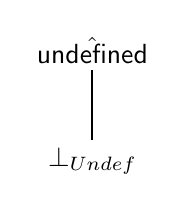
\begin{tikzpicture}
    \node (top) at (0,0) {$\aundef$};
    \node (down) at (0,-1.4) {$\bot_{Undef}$};
    \draw [black, thick, shorten <= -1pt, shorten >=-1pt] (top) -- (down);
  \end{tikzpicture}
\end{matrix}
\quad
\abs{Null} =
\begin{matrix}
  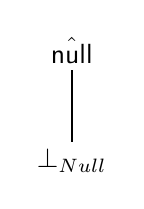
\begin{tikzpicture}
    \node (top) at (0,0) {$\anull$};
    \node (down) at (0,-1.4) {$\bot_{Null}$};
    \draw [black, thick, shorten <= -1pt, shorten >=-1pt] (top) -- (down);
  \end{tikzpicture}
\end{matrix}
\quad
\abs{Bool} =
\begin{matrix}
  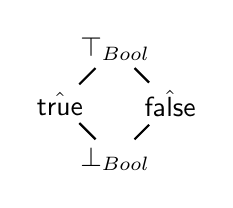
\begin{tikzpicture}
    \node (top) at (0,0) {$\top_{Bool}$};
    \node (midleft) at (-0.7,-0.7) {$\atrue$};
    \node (midright) at (0.7,-0.7) {$\afalse$};
    \node (down) at (0,-1.4) {$\bot_{Bool}$};
    \draw [black, thick, shorten <= -1pt, shorten >=-1pt] (top) -- (midleft);
    \draw [black, thick, shorten <= -1pt, shorten >=-1pt] (top) -- (midright);
    \draw [black, thick, shorten <= -1pt, shorten >=-1pt] (midleft) -- (down);
    \draw [black, thick, shorten <= -1pt, shorten >=-1pt] (midright) -- (down);
  \end{tikzpicture}
\end{matrix}
\quad
\abs{Absent} =
\begin{matrix}
  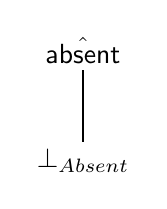
\begin{tikzpicture}
    \node (top) at (0,0) {$\hat{\SF{absent}}$};
    \node (down) at (0,-1.4) {$\bot_{Absent}$};
    \draw [black, thick, shorten <= -1pt, shorten >=-1pt] (top) -- (down);
  \end{tikzpicture}
\end{matrix}
\]
\[
\abs{Number} = 
\begin{matrix} 
  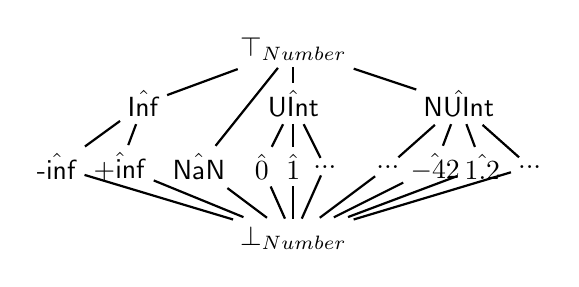
\begin{tikzpicture}
    % First, locate each of the nodes and name them
    \node (top) at (0,0) {$\top_{Number}$};
    \node (upperleft) at (-1.9,-0.7) {$\hat{\SF{Inf}}$};
    \node (uppercenter) at (0,-0.7) {$\hat{\SF{UInt}}$};
    \node (upperright) at (2.1,-0.7) {$\hat{\SF{NUInt}}$};
    \node (lower1) at (-3.0,-1.5) {$\hat{\SF{-inf}}$};
    \node (lower2) at (-2.2,-1.5) {$\hat{\SF{+inf}}$};
    \node (lower3) at (-1.2,-1.5) {$\hat{\SF{NaN}}$};
    \node (lower4) at (-0.4,-1.5) {$\hat{0}$};
    \node (lower5) at (0,-1.5) {$\hat{1}$};
    \node (lower6) at (0.4,-1.5) {...};
    \node (lower7) at (1.2,-1.5) {...};
    \node (lower8) at (1.8,-1.5) {$\hat{-42}$};
    \node (lower9) at (2.4,-1.5) {$\hat{1.2}$};
    \node (lower10) at (3,-1.5) {...};
    \node (down) at (0,-2.4) {$\bot_{Number}$};
    % Now draw the lines0
    \draw [black, thick, shorten <= -1pt, shorten >=-1pt] (top) -- (upperleft);
    \draw [black, thick, shorten <= -1pt, shorten >=-1pt] (top) -- (uppercenter);
    \draw [black, thick, shorten <= -1pt, shorten >=-1pt] (top) -- (upperright);
    \draw [black, thick, shorten <= -1pt, shorten >=-1pt] (top) -- (lower3);
    \draw [black, thick, shorten <= -1pt, shorten >=-1pt] (upperleft) -- (lower1);
    \draw [black, thick, shorten <= -1pt, shorten >=-1pt] (upperleft) -- (lower2);
    \draw [black, thick, shorten <= -1pt, shorten >=-1pt] (uppercenter) -- (lower4);
    \draw [black, thick, shorten <= -1pt, shorten >=-1pt] (uppercenter) -- (lower5);
    \draw [black, thick, shorten <= -1pt, shorten >=-1pt] (uppercenter) -- (lower6);
    \draw [black, thick, shorten <= -1pt, shorten >=-1pt] (upperright) -- (lower7);
    \draw [black, thick, shorten <= -1pt, shorten >=-1pt] (upperright) -- (lower8);
    \draw [black, thick, shorten <= -1pt, shorten >=-1pt] (upperright) -- (lower9);
    \draw [black, thick, shorten <= -1pt, shorten >=-1pt] (upperright) -- (lower10);
    \draw [black, thick, shorten <= -1pt, shorten >=-1pt] (lower1) -- (down);
    \draw [black, thick, shorten <= -1pt, shorten >=-1pt] (lower2) -- (down);
    \draw [black, thick, shorten <= -1pt, shorten >=-1pt] (lower3) -- (down);
    \draw [black, thick, shorten <= -1pt, shorten >=-1pt] (lower4) -- (down);
    \draw [black, thick, shorten <= -1pt, shorten >=-1pt] (lower5) -- (down);
    \draw [black, thick, shorten <= -1pt, shorten >=-1pt] (lower6) -- (down);
    \draw [black, thick, shorten <= -1pt, shorten >=-1pt] (lower7) -- (down);
    \draw [black, thick, shorten <= -1pt, shorten >=-1pt] (lower8) -- (down);
    \draw [black, thick, shorten <= -1pt, shorten >=-1pt] (lower9) -- (down);
    \draw [black, thick, shorten <= -1pt, shorten >=-1pt] (lower10) -- (down);
  \end{tikzpicture}
\end{matrix}
\]
\[
\abs{String} = 
	\begin{matrix} 
		\begin{tikzpicture}
	    % First, locate each of the nodes and name them
	    \node (top) at (0,0) {$\top_{String}$};
	    \node (upperleft) at (-1,-0.7) {$\hat{\SF{UIntStr}}$};
	    \node (upperright) at (1,-0.7) {$\hat{\SF{NUIntStr}}$};
	    \node (lower1) at (-2,-1.5) {$\hat{``0"}$};
	    \node (lower2) at (-1.2,-1.5) {$\hat{``1"}$};
	    \node (lower3) at (-0.4,-1.5) {...};
	    \node (lower4) at (0.4,-1.5) {$\hat{``foo"}$};
	    \node (lower5) at (1.5,-1.5) {$\hat{``bar"}$};
	   	\node (lower6) at (2.2,-1.5) {...};
	    \node (down) at (0,-2.4) {$\bot_{String}$};
	    % Now draw the lines0
	  	\draw [black, thick, shorten <= -1pt, shorten >=-1pt] (top) -- (upperleft);
	  	\draw [black, thick, shorten <= -1pt, shorten >=-1pt] (top) -- (upperright);
	  	\draw [black, thick, shorten <= -1pt, shorten >=-1pt] (midleft) -- (lower1);
	  	\draw [black, thick, shorten <= -1pt, shorten >=-1pt] (midleft) -- (lower2);
	  	\draw [black, thick, shorten <= -1pt, shorten >=-1pt] (midleft) -- (lower3);
	  	\draw [black, thick, shorten <= -1pt, shorten >=-1pt] (midright) -- (lower4);
	  	\draw [black, thick, shorten <= -1pt, shorten >=-1pt] (midright) -- (lower5);
	  	\draw [black, thick, shorten <= -1pt, shorten >=-1pt] (midright) -- (lower6);
	  	\draw [black, thick, shorten <= -1pt, shorten >=-1pt] (lower1) -- (down);
	  	\draw [black, thick, shorten <= -1pt, shorten >=-1pt] (lower2) -- (down);
	  	\draw [black, thick, shorten <= -1pt, shorten >=-1pt] (lower3) -- (down);
	  	\draw [black, thick, shorten <= -1pt, shorten >=-1pt] (lower4) -- (down);
	  	\draw [black, thick, shorten <= -1pt, shorten >=-1pt] (lower5) -- (down);
	  	\draw [black, thick, shorten <= -1pt, shorten >=-1pt] (lower6) -- (down);
		\end{tikzpicture}
	\end{matrix}
\]

% % States                         
% \[
% \powerset{\State} \galois{\alpha_{state}}{\gamma_{state}} \abs{State}
% \]
% \[
% \begin{array}{lcl}
% \alpha_{state}(S) & = & (\hat{H})\\
% &&  \wherec{
%     \hat{H} = \alpha_{Heap}\left(\set{H \mid (H,A)\in S}\right) \\
% %    \hat{AS} = \bigcup\set{\alpha_{Env}(A) \mid (H,A)\in S} \\
%   } \\
% \end{array}
% \]

% % Heap
% \[
% \powerset{\Heap} \galois{\alpha_{heap}}{\gamma_{heap}} \aHeap
% \]
% \[
% \begin{array}{lcl}
% \alpha_{heap}(HS) & = & 
% \lambda \hat{l}.\alpha_{Obj}(\{o~\mid~ \hat{l}=\alpha_{Loc}(l) \land l\mapsto o\in HS \})
% \end{array}
% \]

% % Env
% \[
% \SF{Env} \galois{\alpha_{env}}{\gamma_{env}} \abs{Env}
% \]

% % Obj
% \[
% \powerset{\Obj} \galois{\alpha_{Obj}}{\gamma_{obj}} \aObj
% \]

% % PropValue
% \[
% \powerset{\SF{PropValue}} \galois{\alpha_{PropValue}}{\gamma_{PropValue}} \abs{PropValue}
% \]

% % ObjectValue
% \[
% \powerset{\SF{ObjectValue}} \galois{\alpha_{ObjectValue}}{\gamma_{ObjectValue}} \abs{ObjectValue}
% \]

% % Value
% \[
% \powerset{\Value} \galois{\alpha_{Value}}{\gamma_{Value}} \aValue
% \]

% % PValue
% \[
% \powerset{\PValue} \galois{\alpha_{PValue}}{\gamma_{PValue}} \abs{PValue}
% \]

\subsection{Domain Operators}
\[
\begin{array}{ll}
\textit{Heap Order} & : \aHeap \times \aHeap \rightarrow \SF{Boolean} \\
& \hat{H}_1 \sqsubseteq \hat{H}_2 \defi \forall \hat{l} \in dom(\hat{H}_1):
      \hat{H}_1(\hat{l}) \sqsubseteq \hat{H}_2(\hat{l})
\\

\textit{Heap Join} & : \aHeap \times \aHeap \rightarrow \aHeap \\
& \hat{H}_1 \sqcup \hat{H}_2  \defi \forall \hat{l} \in dom(\hat{H}_1) \cup dom(\hat{H}_2): 
  \left\{
    \begin{array}{ll}
      \left[\hat{l} \mapsto \hat{H}_1(\hat{l}) \sqcup \hat{H}_2(\hat{l})\right] & \ifc{\hat{l} \in dom(\hat{H}_1)\land \hat{l} \in dom(\hat{H}_2)}\\
      \left[\hat{l} \mapsto \hat{H}_2(\hat{l}) \right] & \ifc{\hat{l} \not\in dom(\hat{H}_1)\land \hat{l} \in dom(\hat{H}_2)}\\
      \left[\hat{l} \mapsto \hat{H}_1(\hat{l}) \right] & \ifc{\hat{l} \in dom(\hat{H}_1)\land \hat{l} \not\in dom(\hat{H}_2)}\\
    \end{array}
  \right.\\
\textit{Heap Domain In} & : \aHeap \times \aLoc \rightarrow \SF{Boolean} \\
& \hat{l} \in dom(\hat{H}) \defi
 \left\{
   \begin{array}{ll}
     \SF{true}
     & \ifc{\hat{l} \in \{ \hat{l}'\ |\ (\hat{l}', \hat{o}) \in \hat{H}\}} \\
     \SF{false}
     & \owc \\
   \end{array}
 \right.\\

\textit{Heap Update} & : \aHeap \times \aLoc \times \aObj \rightarrow \aHeap \\
& \hat{H}[\hat{l} \mapsto \hat{o}] \defi
 \left\{
   \begin{array}{ll}
      \{( \hat{l}, \hat{o})\} \cup (\hat{H}-\hat{l})
      & \ifc{\hat{l} = \hat{l}_R} \\
      \{( \hat{l}, \hat{H}(\hat{l}) \sqcup \hat{o})\} \cup (\hat{H}-\hat{l})
     & \ifc{\hat{l} = \hat{l}_O} \\
   \end{array}
 \right.\\
\\
\textit{Obj Order} & : \aObj \times \aObj \rightarrow \SF{Boolean} \\
& \hat{o}_1 \sqsubseteq \hat{o}_2 \defi \forall x \in dom(\hat{o}_1) \cup dom(\hat{o}_2): \hat{o}_1(x) \sqsubseteq \hat{o}_2(x)\\
\\
\textit{Obj Join} & : \aObj \times \aObj \rightarrow \aObj \\
& \hat{o}_1 \sqcup \hat{o}_2  \defi \forall x \in dom(\hat{o}_1) \cup dom(\hat{o}_2): \left[x \mapsto \hat{o}_1(x) \sqcup \hat{o}_2(x)\right]\\
\\

\textit{Obj Domain In} & : \aObj \times \abs{String} \rightarrow \abs{Bool} \\
& \hat{s} \dot{\in} dom(\hat{o}) \defi
     \left\{
       \begin{array}{ll}
         x \dot{\in} dom(\hat{o})
         & \ifc{\hat{s} = \hat{\SF{UIntStrSingle}}(x) }\\
         x \dot{\in} dom(\hat{o})
         & \ifc{\hat{s} = \hat{\SF{NUIntStrSingle}}(x) }\\
         \hat{b}_1
         & \ifc{\hat{s} = \hat{\SF{UIntStr}} }\\
         \hat{b}_2
         & \ifc{\hat{s} = \hat{\SF{NUIntStr}} }\\
         \hat{b}_3
         & \ifc{\hat{s} = \top_{String} }\\
         \bot_{Bool} 
         &\ifc{\hat{s} = \bot_{String} }\\
       \end{array}
     \right.\\
 & \quad\wherec{
   \hat{b}_1 = 
     \left\{
       \begin{array}{ll}
         \top_{Bool} & \ifc{\hat{o}(\emph{@default\_UInt}).1.1.1 \not\sqsubseteq \bot_{Value}}\\
         \top_{Bool} & \ifc{\hat{o}(\emph{@default\_UInt}).1.1.1 \sqsubseteq \bot_{Value}}\\
                     & \quad \land\ \exists x \in dom(\hat{o}):x \in \SF{String} \land \hat{``x"} \sqsubseteq \hat{\SF{UIntStr}}\\
         \afalse & \owc\\
       \end{array}
     \right.\\
   \hat{b}_2 = 
     \left\{
       \begin{array}{ll}
         \top_{Bool} & \ifc{\hat{o}(\emph{@default\_NUInt}).1.1.1 \not\sqsubseteq \bot_{Value}}\\
         \top_{Bool} & \ifc{\hat{o}(\emph{@default\_NUInt}).1.1.1 \sqsubseteq \bot_{Value}}\\
                     & \quad \land\ \exists x \in dom(\hat{o}):x \in \SF{String} \land \hat{``x"} \sqsubseteq \hat{\SF{NUIntStr}}\\
         \afalse & \owc\\
       \end{array}
     \right.\\
   \hat{b}_3 = 
     \left\{
       \begin{array}{ll}
         \top_{Bool} 
         & \ifc{\hat{o}(\emph{@default\_UInt}).1.1.1 \not\sqsubseteq \bot_{Value}\vee \hat{o}(\emph{@default\_NUInt}).1.1.1 \not\sqsubseteq \bot_{Value}}\\
         \top_{Bool} 
         & \ifc{\hat{o}(\emph{@default\_UInt}).1.1.1 \sqsubseteq \bot_{Value}\land \hat{o}(\emph{@default\_NUInt}).1.1.1 \sqsubseteq \bot_{Value}}\\
         & \quad \land\ \exists x \in dom(\hat{o}):x \in \SF{String}\\
         \afalse & \owc\\
       \end{array}
     \right.\\ 
  }\\
\end{array}
\]

\[
\begin{array}{ll}
\textit{Obj Domain In} & : \aObj \times \Prop \rightarrow \abs{Bool} \\
& x \dot{\in} dom(\hat{o}) \defi
  \left\{
    \begin{array}{ll}
      \atrue
      &\ifc{\hat{o}(x)\not\sqsubseteq\bot \land \hat{\SF{absent}}\not\sqsubseteq\hat{o}(x).2}\\
      \top_{Bool}
      &\ifc{\hat{o}(x)\not\sqsubseteq\bot \land \hat{\SF{absent}}\sqsubseteq\hat{o}(x).2}\\
      \top_{Bool}
      &\ifc{\hat{o}(x)\sqsubseteq\bot \land x\in \SF{String} \land \alpha(x) \sqsubseteq \hat{\SF{UIntStr}}}\\
      & \quad\land \hat{o}(\emph{@default\_UInt}).1.1.1 \not\sqsubseteq \bot_{Value} \\
      \top_{Bool}
      &\ifc{\hat{o}(x)\sqsubseteq\bot \land x\in \SF{String} \land \alpha(x) \sqsubseteq \hat{\SF{NUIntStr}}}\\
      & \quad\land \hat{o}(\emph{@default\_NUInt}).1.1.1 \not\sqsubseteq \bot_{Value} \\
      \afalse
      &\ifc{\hat{o}(x)\sqsubseteq\bot \land x\in \SF{String} \land \alpha(x) \sqsubseteq \hat{\SF{UIntStr}}}\\
      & \quad\land \hat{o}(\emph{@default\_UInt}).1.1.1 \sqsubseteq \bot_{Value} \\
      \afalse
      &\ifc{\hat{o}(x)\sqsubseteq\bot \land x\in \SF{String} \land \alpha(x) \sqsubseteq \hat{\SF{NUIntStr}}}\\
      & \quad\land \hat{o}(\emph{@default\_NUInt}).1.1.1 \sqsubseteq \bot_{Value} \\
      \afalse
      &\ifc{\hat{o}(x)\sqsubseteq\bot \land x\not\in \SF{String}}\\
      \afalse&\owc\\
    \end{array}
  \right.\\
\\\\

\textit{Obj Lookup} & : \aObj \times \abs{String} \rightarrow \abs{PropValue} \times \abs{Absent}\\
& \hat{o}(s) \defi
     \left\{
       \begin{array}{ll}
         \hat{o}(x)
         & \ifc{\hat{s} = \hat{\SF{UIntStrSingle}}(x) }\\
         \hat{o}(x)
         & \ifc{\hat{s} = \hat{\SF{NUIntStrSingle}}(x) }\\
         \langle (\bigsqcup_{x \in P_1} \hat{o}(x)).1 \sqcup \hat{o}(\emph{@default\_UInt}).1, \top_{Absent}\rangle
         & \ifc{\hat{s} = \hat{\SF{UIntStr}} }\\
         \langle (\bigsqcup_{x \in P_2} \hat{o}(x)).1 \sqcup \hat{o}(\emph{@default\_NUInt}).1, \top_{Absent}\rangle
         & \ifc{\hat{s} = \hat{\SF{NUIntStr}} }\\
         \left\langle 
           \begin{matrix}
             (\bigsqcup_{x \in P_3} \hat{o}(x)).1 \sqcup \hat{o}(\emph{@default\_UInt}).1 \\ 
             \sqcup \hat{o}(\emph{@default\_NUInt}).1
           \end{matrix},
         \top_{Absent}\right\rangle
         & \ifc{\hat{s} = \top_{String} }\\
         \bot_{PropValue \times Absent} 
         &\ifc{\hat{s} = \bot_{String} }\\
       \end{array}
     \right.\\
 & \quad\wherec{
   P_1 = \{ x\ |\ x \in dom(\hat{o}) \land x \in \SF{String} \land \hat{``x"} \sqsubseteq \hat{\SF{UIntStr}}\}\\
   P_2 = \{ x\ |\ x \in dom(\hat{o}) \land x \in \SF{String} \land \hat{``x"} \sqsubseteq \hat{\SF{NUIntStr}}\}\\
   P_3 = \{ x\ |\ x \in dom(\hat{o}) \land x \in \SF{String}\}\\
  }\\
\\\\
\textit{Obj Lookup} & : \aObj \times \Prop \rightarrow \abs{PropValue} \times \abs{Absent} \\
& \hat{o}(x) \defi 
  \left\{
    \begin{array}{ll}
      \langle\hat{propv}, \hat{abs}\rangle
      & \ifc{x \rightarrow \langle\hat{propv}, \hat{abs}\rangle \in \hat{o}} \\
      \langle\bot_{PropValue}, \bot_{Absent}\rangle
      & \ifc{x \rightarrow \langle\hat{propv}, \hat{abs}\rangle \not\in \hat{o}} \land x \not\in \SF{String}\\
      \langle\hat{propv}_2, \top_{Absent}\rangle
      & \ifc{x \rightarrow \langle\hat{propv}_1, \hat{abs}_1\rangle \not\in \hat{o}\land \alpha(x) \sqsubseteq \hat{\SF{UIntStr}}}\\
      & \quad\land \emph{@default\_UInt} \rightarrow \langle\hat{propv}_2, \hat{abs}_2\rangle \in \hat{o} \land x \in \SF{String}\\
      \langle\hat{propv}_3, \top_{Absent}\rangle
      & \ifc{x \rightarrow \langle\hat{propv}_1, \hat{abs}_1\rangle \not\in \hat{o}\land \alpha(x) \sqsubseteq \hat{\SF{NUIntStr}}}\\
      & \quad\land \emph{@default\_NUInt} \rightarrow \langle\hat{propv}_3, \hat{abs}_3\rangle \in \hat{o} \land x \in \SF{String}\\
    \end{array}
  \right.\\
\\
\end{array}
\]

\[
\begin{array}{ll}
\textit{Obj Update} & : \aObj \times \abs{String} \times \abs{PropValue} \rightarrow \aObj \\
& \hat{o}[\hat{s} \mapsto \hat{propv}] \defi 
 \left\{
       \begin{array}{ll}
         \hat{o}[x \mapsto \hat{propv}]
         & \ifc{\hat{s} = \hat{\SF{UIntStrSingle}}(x) }\\
         \hat{o}[x \mapsto \hat{propv}]
         & \ifc{\hat{s} = \hat{\SF{NUIntStrSingle}}(x) }\\
         \hat{o}
         \left[
           \begin{array}{l}
           \forall x \in P_1 : x \mapsto \hat{o}(x) \sqcup \hat{propv},\\
           \emph{@default\_UInt} \mapsto \hat{o}(\emph{@default\_UInt}) \sqcup \hat{propv}\\
           \end{array}
         \right]
         & \ifc{\hat{s} = \hat{\SF{UIntStr}} }\\
         \hat{o}
         \left[
           \begin{array}{l}
           \forall x \in P_2 : x \mapsto \hat{o}(x) \sqcup \hat{propv},\\
           \emph{@default\_NUInt} \mapsto \hat{o}(\emph{@default\_NUInt}) \sqcup \hat{propv}\\
           \end{array}
         \right]
         & \ifc{\hat{s} = \hat{\SF{NUIntStr}} }\\
         \hat{o}
         \left[
           \begin{array}{l}
           \forall x \in P_3 : x \mapsto \hat{o}(x) \sqcup \hat{propv},\\
           \emph{@default\_UInt} \mapsto \hat{o}(\emph{@default\_UInt}) \sqcup \hat{propv},\\
           \emph{@default\_NUInt} \mapsto \hat{o}(\emph{@default\_NUInt}) \sqcup \hat{propv}\\
           \end{array}
         \right]
         & \ifc{\hat{s} = \top_{String} }\\
         \bot_{Obj}
         &\ifc{\hat{s} = \bot_{String} }\\
       \end{array}
     \right.\\
& \quad\wherec{
   P_1 = \{ x\ |\ x \in dom(\hat{o}) \land x \in \SF{String} \land \hat{``x"} \sqsubseteq \hat{\SF{UIntStr}}\}\\
   P_2 = \{ x\ |\ x \in dom(\hat{o}) \land x \in \SF{String} \land \hat{``x"} \sqsubseteq \hat{\SF{NUIntStr}}\}\\
   P_3 = \{ x\ |\ x \in dom(\hat{o}) \land x \in \SF{String}\}\\
  }\\
\\\\
\textit{Obj Update} & : \aObj \times \Prop \times \abs{PropValue} \rightarrow \aObj \\
& \hat{o}[x \mapsto \hat{propv}] = \{( x, \langle \hat{propv}, \bot_{Absent} \rangle)\} \cup (\hat{o}\setminus\{(x,\langle \hat{propv}', \hat{abs}' \rangle)\})\\
\\\\
\textit{Obj Remove} & : \aObj \times \abs{String} \rightarrow \aObj \\
& \hat{o}- \hat{s} \defi 
 \left\{
       \begin{array}{ll}
         \{ (y,\langle \hat{propv}, \hat{abs}\rangle)\ |\ (y,\langle \hat{propv}, \hat{abs}\rangle) \in \hat{o} \land y \neq x \}
         & \ifc{\hat{s} = \hat{\SF{UIntStrSingle}}(x) }\\
         \{ (y,\langle \hat{propv}, \hat{abs}\rangle)\ |\ (y,\langle \hat{propv}, \hat{abs}\rangle) \in \hat{o} \land y \neq x \}
         & \ifc{\hat{s} = \hat{\SF{NUIntStrSingle}}(x) }\\
         \bigsqcup_{x \in P_1}\ \{ (y,\langle \hat{propv}, \hat{abs}\rangle)\ |\ (y,\langle \hat{propv}, \hat{abs}\rangle) \in \hat{o} \land y \neq x \}
         & \ifc{\hat{s} = \hat{\SF{UIntStr}} }\\
         \bigsqcup_{x \in P_2}\ \{ (y,\langle \hat{propv}, \hat{abs}\rangle)\ |\ (y,\langle \hat{propv}, \hat{abs}\rangle) \in \hat{o} \land y \neq x \}
         & \ifc{\hat{s} = \hat{\SF{NUIntStr}} }\\
         \bigsqcup_{x \in P_3}\ \{ (y,\langle \hat{propv}, \hat{abs}\rangle)\ |\ (y,\langle \hat{propv}, \hat{abs}\rangle) \in \hat{o} \land y \neq x \}
         & \ifc{\hat{s} = \top_{String} }\\
         \hat{o}
         & \ifc{\hat{s} = \bot_{String} }\\
       \end{array}
     \right.\\
& \quad\wherec{
   P_1 = \{ x\ |\ x \in dom(\hat{o}) \land x \in \SF{String} \land \hat{``x"} \sqsubseteq \hat{\SF{UIntStr}}\}\\
   P_2 = \{ x\ |\ x \in dom(\hat{o}) \land x \in \SF{String} \land \hat{``x"} \sqsubseteq \hat{\SF{NUIntStr}}\}\\
   P_3 = \{ x\ |\ x \in dom(\hat{o}) \land x \in \SF{String}\}\\
  }\\
\\

\end{array}
\]


\subsection{Helper Functions}
{\inblue\tt .../jsaf/analysis/typing/Helper.scala}

\[
\begin{array}{ll}
\ahf{IsArray} & : \aHeap \times \aLoc \rightarrow \abs{Bool} \\
& {\inblue \hat{H}(\hat{l})(\varprop{class}).1.2\textit{ is the }\abs{Value}} \\
& \ahf{IsArray}(\hat{H},\hat{l}) = \hat{b}_1\sqcup\hat{b}_2\\
& \quad\wherec{
    \hat{b}_1=\left\{
      \begin{array}{ll}
        \atrue &\ifc{\hat{``Array"} \sqsubseteq \hat{H}(\hat{l})(\varprop{class}).1.2}\\
        \bot_{Bool} & \owc \\
      \end{array}
    \right.\\
    \hat{b}_2 = \left\{
      \begin{array}{ll}
        \afalse & \ifc{\hat{``Array"} \neq \hat{H}(\hat{l})(\varprop{class}).1.2}\\
        \bot_{Bool} & \owc\\
      \end{array}
    \right.\\
  }\\
\\
\end{array}
\]

\[
\begin{array}{ll}
\ahf{IsObject} & : \aHeap \times \aLoc \rightarrow \abs{Bool} \\
& \ahf{IsObject}(\hat{H},\hat{l}) = \hat{b}_1\sqcup\hat{b}_2\\
& \quad\wherec{
    \hat{b}_1=\left\{
      \begin{array}{ll}
        \atrue &\ifc{\hat{``Object"} \sqsubseteq \hat{H}(\hat{l})(\varprop{class}).1.2 \lor
          \hat{``Function"} \sqsubseteq \hat{H}(\hat{l})(\varprop{class}).1.2
        }\\
        \bot_{Bool} & \owc \\
      \end{array}
    \right.\\
    \hat{b}_2 = \left\{
      \begin{array}{ll}
        \afalse & \ifc{\hat{``Object"} \neq \hat{H}(\hat{l})(\varprop{class}).1.2 \land
          \hat{``Function"} \neq \hat{H}(\hat{l})(\varprop{class}).1.2
        }\\
        \bot_{Bool} & \owc\\
      \end{array}
    \right.\\
}\\
\\

\ahf{IsArrayIndex} & : \aValue \rightarrow \abs{Bool} \\
& \ahf{IsArrayIndex}(\hat{v}) = \left\{
      \begin{array}{ll}
        \atrue
        &\ifc{\hat{v}\not\sqsubseteq\bot_{String} \land \hat{v}\sqsubseteq\hat{\SF{UIntStr}} \\
        }\\
        \afalse
        & \ifc{\hat{v}\not\sqsubseteq\bot_{String} \land \hat{v}\sqsubseteq\hat{\SF{NUIntStr}} \\
        }\\
        \bot_{Bool} & \ifc{\hat{v}\sqsubseteq\bot_{Value}} \\
        \top_{Bool} & \owc \\
      \end{array}
    \right.\\
\\

\ahf{VarStore} & : \aHeap \times \Prop \times \aValue
\times \abs{Bool} \rightarrow \aHeap \\
& \ahf{VarStore}(\hat{H}, x, \hat{v}, \hat{b})
  =
  \hat{H}_1 \sqcup \hat{H}_2 \\
&\wherec{
  \hat{l}_g = \avarloc{Global}_R\ \land\ \hat{ov}_{old} = \hat{H}(\hat{l}_g)(x).1.1\\
  \hat{H}_1 =
  \left\{
    \begin{array}{ll}
      \ahf{PropStore}(\hat{H},\hat{l}_g,\hat{x},\hat{v}) & \ifc{\afalse\sqsubseteq(x \dot{\in} dom(\hat{H}(\hat{l}_g)))} \\
      \bot_{Heap} & \owc \\
    \end{array}
   \right.\\ 
  \hat{H}_2 =
  \left\{
    \begin{array}{ll}
      \hat{H}[\hat{l}_g\mapsto \hat{H}(\hat{l}_g)[x \mapsto
        \langle \hat{v},\hat{b},\hat{ov}_{old}.3,\hat{ov}_{old}.4\rangle]]
        & \ifc{
          \atrue\sqsubseteq (x \dot{\in} dom(\hat{H}(\hat{l}_g)))\\
        } \\
        \bot_{Heap} & \owc \\
    \end{array}
  \right. \\
}\\
\\
% & \ahf{VarStore}(\hat{H},\hat{l}_{hd}::\hat{l}_{tl}^{*},x,\hat{v},\hat{b})
%   =  \hat{H}\sqcup\hat{H}[\hat{l}_{hd}\mapsto \hat{H}(\hat{l}_{hd})[x\mapsto \set{\hat{H}(\hat{l}_{hd})(x) \rwith value=\hat{v}; writable=\hat{b}}]]\\
% & \quad\ifc{x \in \ahf{Dom}(\hat{H}(\hat{l}_{hd}))}\\
% & \ahf{VarStore}(\hat{H},\hat{l}_{hd}::\hat{l}_{tl}^{*},x,\hat{v},\hat{b})
%   =  \ahf{VarStore}(\hat{H},\hat{l}_{tl}^{*},x,\hat{v},\hat{b})\\
% & \quad\ifc{x \not\in \ahf{Dom}(\hat{H}(\hat{l}_{hd}))}\\\\

\ahf{PropStore} & : \aHeap \times \aLoc \times \abs{String} \times \aValue \rightarrow \aHeap \\
& \ahf{PropStore}(\hat{H},\hat{l},\hat{s},\hat{v})
  = \hat{H}_1\sqcup\hat{H}_2\\
& \quad\wherec{
\hat{H}_1 = \left\{
    \begin{array}{ll}
      \hat{H}\left[\hat{l}\mapsto \hat{H}(\hat{l})\left[\hat{s}\mapsto \langle\hat{v},\atrue,\atrue,\atrue\rangle\right]\right] & \ifc{\afalse\sqsubseteq(\hat{s} \dot{\in} dom(\hat{H}(\hat{l})))} \\
      \bot_{Heap} & \owc \\
    \end{array}
  \right. \\
  \hat{ov}_{old}=\hat{H}(\hat{l})(\hat{s}).1.1\\
  \hat{H}_2 = \left\{
    \begin{array}{ll}
      \hat{H}\left[\hat{l}\mapsto \hat{H}(\hat{l})\left[\hat{s}\mapsto
          \langle \hat{v},\hat{ov}_{old}.2,\hat{ov}_{old}.3,\hat{ov}_{old}.4\rangle
% \set{H(l)(x)\rwith value=v}
        \right]\right] & \ifc{\atrue\sqsubseteq (\hat{s} \dot{\in} dom(\hat{H}(\hat{l})))}\\
      \bot_{Heap} & \owc \\
    \end{array}
  \right. \\
}\\
\\


& {\inblue \hat{H}(\hat{l})(\hat{s}).1.1.4\textit{ means the configurable attribute of the property.}} \\
\ahf{Delete} & : \aHeap \times \aLoc \times \abs{String} \rightarrow \aHeap
\times \abs{Bool}\\
& \ahf{Delete}(\hat{H},\hat{l},\hat{s})
  = (\hat{H}_1\sqcup\hat{H}_2,\hat{b}_1\sqcup\hat{b}_2)\\
&  \quad\wherec{
%    (\hat{H}_1,\hat{b}_1) = \left\{
%      \begin{array}{ll}
%        (\hat{H},\atrue)
%        & \ifc{\afalse\sqsubseteq\ahf{HasOwnProperty}(\hat{H},\hat{l},x)} \\
%        \bot_{Heap\times Bool} & \owc \\
%      \end{array}
%    \right.\\
    (\hat{H}_1,\hat{b}_1) = \left\{
      \begin{array}{ll}
        (\hat{H},\afalse)
        & \ifc{\atrue\sqsubseteq\ahf{HasOwnProperty}(\hat{H},\hat{l},\hat{s})
          \land\ \afalse\sqsubseteq\hat{H}(\hat{l})(\hat{s}).1.1.4}\\
        \bot_{Heap\times Bool} & \owc \\
      \end{array}
    \right.\\
%{\inblue \textit{If the value is deleted in update operation,}}\\
%{\inblue \textit{the absent attribute of the value will be 'absent' instead of removing the value}}\\
%{\inblue \textit{because of a weak update.}}\\
    (\hat{H}_2,\hat{b}_2) = \left\{
      \begin{array}{ll}
        (\hat{H}[\hat{l}\mapsto \hat{H}(\hat{l}) - \hat{s}],\atrue)
        & \ifc{
          \begin{array}{l}
            \left(
              \begin{array}{l}
              \atrue \sqsubseteq\ahf{HasOwnProperty}(\hat{H},\hat{l},\hat{s})\\
              \land \atrue\sqsubseteq\hat{H}(\hat{l})(\hat{s}).1.1.4)
              \end{array}
            \right)\\
            \vee (\afalse\sqsubseteq\ahf{HasOwnProperty}(\hat{H},\hat{l},\hat{s}))
          \end{array}}\\
        \bot_{Heap\times Bool} & \owc \\
      \end{array}
    \right.\\
  }\\
\\
\end{array}
\]

\[
\begin{array}{ll}

\ahf{Lookup} & : \aHeap \times \Prop \rightarrow \aValue \times \powerset{\abs{Exception}}\\
&
  \ahf{Lookup}(\hat{H},x)
   = (\hat{v}_1\sqcup\hat{v}_2, \hat{es})\\
& \quad\wherec{
  \hat{v}_1 = \left\{
    \begin{array}{ll}
      \hat{H}(\avarloc{Global}_R)(x).1.1.1
      & \ifc{\atrue\sqsubseteq(x \dot{\in} dom(\hat{H}(\avarloc{Global})))} \\
      \bot_{Value}
      & \owc \\
    \end{array}\right. \\
  (\hat{v}_2, \hat{es}) = \left\{
    \begin{array}{ll}
      (\hat{v}_3, \hat{exc})
      & \ifc{\vfalse\sqsubseteq(x \dot{\in} dom(\hat{H}(\avarloc{Global})))}\\
      (\bot_{Value}, \{\})
      & \owc \\
    \end{array}\right. \\
  \hat{L}_{proto} = \hat{H}(\avarloc{Global}_R)(\hat{\varprop{proto}}).1.1.1.2\\
  \hat{v}_3 = 
    \bigsqcup_{\hat{l}_{proto}\in\hat{L}_{proto}}
    \left\{
    \begin{array}{ll}
      \ahf{Proto}(\hat{H}, \hat{l}_{proto}, \hat{x})
      & \ifc{\atrue\sqsubseteq\ahf{HasProperty}(\hat{H},\hat{l}_{proto},\hat{x})}\\
      \bot_{Value}
      & \owc \\
    \end{array}\right. \\
  \hat{exc} = 
    \bigsqcup_{\hat{l}_{proto}\in\hat{L}_{proto}}
    \left\{
    \begin{array}{ll}
      \{\hat{\SF{ReferenceError}}\}
      & \ifc{\afalse\sqsubseteq\ahf{HasProperty}(\hat{H},\hat{l}_{proto},\hat{x})}\\
      \bot_{Exception}
      & \owc \\
    \end{array}\right. \\
}\\
\\

& {\inblue \textit{For all case of }\hat{s}_n\textit{ if the condition is false, the value of }\hat{s}_n\textit{ is }\bot_{String}.} \\
\ahf{TypeTag} & : \aHeap \times \aValue \rightarrow \abs{String}\\
& \ahf{TypeTag}(\hat{H},\hat{v}) = \hat{s}_1\sqcup\hat{s}_2\sqcup\hat{s}_3\sqcup\hat{s}_4\sqcup\hat{s}_5\sqcup\hat{s}_6\sqcup\hat{s}_7 \\
& \wherec{
  \begin{array}{ll}
  \hat{s}_1 = \hat{``number"} & \ifc{\hat{v}.1.4\not\sqsubseteq\bot_{number}} \\
  \hat{s}_2 = \hat{``boolean"} & \ifc{\hat{v}.1.3\not\sqsubseteq\bot_{boolean}} \\
  \hat{s}_3 = \hat{``string"} & \ifc{\hat{v}.1.5\not\sqsubseteq\bot_{string}} \\
  \hat{s}_4 = \hat{``object"} & \ifc{\hat{v}.2\not\sqsubseteq\bot_{Loc}\land\afalse\sqsubseteq\bigsqcup_{\hat{l}\in\hat{v}.2}\ahf{IsCallable}(\hat{H},\hat{l})} \\
  \hat{s}_5 = \hat{``function"} & \ifc{\hat{v}.2\not\sqsubseteq\bot_{Loc}\land\atrue\sqsubseteq\bigsqcup_{\hat{l}\in\hat{v}.2}\ahf{IsCallable}(\hat{H},\hat{l})} \\
  \hat{s}_6 = \hat{``object"} & \ifc{\hat{v}.1.2\not\sqsubseteq\bot_{null}} \\
  \hat{s}_7 = \hat{``undefined"} & \ifc{\hat{v}.1.1\not\sqsubseteq\bot_{undef}} \\
  \end{array}\\
  }\\
\\


\ahf{CanPut} & : \aHeap \times \aLoc \times \abs{String} \rightarrow \abs{Bool}\\
&
\begin{array}{ll}
  \ahf{CanPut}(\hat{H},\hat{l},\hat{s}) = \ahf{CanPutHelp}(\hat{H},\hat{l},\hat{s},\hat{l}) & \\
\end{array}
\\\\

%& {\inblue \textit{For all case of }\hat{s}_n\textit{ if the condition is false, the value of }\hat{s}_n\textit{ is }\bot_{String}.} \\
\ahf{CanPutHelp} &  : \aHeap \times \aLoc \times \abs{String} \times \aLoc \rightarrow \abs{Bool}\\
&  \ahf{CanPutHelp}(\hat{H},\hat{l}_1,\hat{s},\hat{l}_2)  = \hat{b}_1\sqcup\hat{b}_2\\
&  \quad\wherec{
    \hat{b}_1 =
    \left\{
      \begin{array}{ll}
        \hat{H}(\hat{l}_1)(\hat{s}).1.1.2
        ~~{\inblue \textit{// writable attribute}}
        & \ifc{\atrue\sqsubseteq(\hat{s} \dot{\in} dom(\hat{h}(\hat{l})))}\\
        \bot_{Bool} & \owc\\
      \end{array}
    \right.\\
    \hat{L}_{proto}=\hat{H}(\hat{l}_1)(\varprop{proto}).1.1.1.2
~~{\inblue \textit{// $\powerset{\aLoc}$ type}}\\
    \hat{b}_2 =
    \left\{
      \begin{array}{ll}
        \hat{b}_3 \sqcup \bigsqcup_{\hat{l}_{proto}\in\hat{L}_{proto}}\ahf{CanPutHelp}(\hat{H},\hat{l}_{proto},\hat{s},\hat{l}_2)& \ifc{\afalse\sqsubseteq(\hat{s} \dot{\in} dom(\hat{h}(\hat{l})))}\\
        \bot_{Bool} & \owc\\
      \end{array}
    \right.\\
    \hat{b}_3 =
    \left\{
      \begin{array}{ll}
        \hat{H}(\hat{l})(\varprop{extensible}).1.2.1.3& \ifc{\hat{H}(\hat{l}_1)(\varprop{proto}).1.1.1.1.2 \not\sqsubseteq \bot_{Null}}\\
        \bot_{Bool} & \owc\\
      \end{array}
    \right.\\
    }\\
\\

\ahf{CanPutVar} & : \aHeap \times \Prop \rightarrow \abs{Bool}\\
&
\begin{array}{ll}
\ahf{CanPutVar}(\hat{H},x)
  =  \hat{b}_1\sqcup\hat{b}_2\\
  \quad\wherec{
    \hat{b}_1 =
      \left\{
        \begin{array}{ll}
          \hat{H}(\avarloc{Global}_R)(x).1.1.2 & \ifc{\atrue\sqsubseteq(x \dot{\in} dom(\hat{H}(\avarloc{Global})))} \\
          \bot_{Bool} & \owc \\
        \end{array}
      \right.\\
    \hat{b}_2 = 
      \left\{
        \begin{array}{ll}
          \ahf{CanPut}(\hat{H},\avarloc{Global}_R,\hat{x}) & \ifc{\afalse\sqsubseteq(x \dot{\in} dom(\hat{H}(\avarloc{Global})))} \\
          \bot_{Bool} & \owc \\
        \end{array}
      \right.\\
  }
\end{array}\\
\\
\end{array}
\]


\[
\begin{array}{ll}

\ahf{HasProperty} & : \aHeap \times \aLoc \times \abs{String} \rightarrow \abs{Bool} \\
& \ahf{HasProperty}(\hat{H},\hat{l},\hat{s}) = \hat{b}_1\sqcup\hat{b}_2 \\
& \wherec{
  \hat{b}_1 = \left\{
    \begin{array}{ll}
      \atrue & \ifc{\atrue\sqsubseteq\ahf{HasOwnProperty}(\hat{H},\hat{l},\hat{s})} \\
      \bot_{Bool} & \owc \\
    \end{array}
    \right.\\
    \hat{L}_{proto} = \hat{H}(\hat{l})(\varprop{proto}).1.1.1.2 \\
  \hat{b}_2 = \left\{
    \begin{array}{ll}
      \hat{b}_3 \sqcup \bigsqcup_{\hat{l}_{proto}\in\hat{L}_{proto}}\ahf{HasProperty}(\hat{H},\hat{l}_{proto},\hat{s})
      & \ifc{\afalse\sqsubseteq\ahf{HasOwnProperty}(\hat{H},\hat{l},\hat{s})} \\
      \bot_{Bool} & \owc \\
    \end{array}
    \right.\\
    \hat{b}_3 =
    \left\{
      \begin{array}{ll}
        \afalse & \ifc{\hat{H}(\hat{l}_1)(\varprop{proto}).1.1.1.1.2 \not\sqsubseteq \bot_{Null}}\\
        \bot_{Bool} & \owc\\
      \end{array}
    \right.\\
  }\\
\\

\ahf{HasOwnProperty} & : \aHeap \times \aLoc \times \abs{String} \rightarrow \abs{Bool} \\
&  \ahf{HasOwnProperty}(\hat{H},\hat{l},\hat{s}) = (\hat{s} \dot{\in} dom(\hat{h}(\hat{l})))\\
\\\\
\ahf{Proto} & : \aHeap \times \aLoc \times \abs{String} \rightarrow \aValue\\
  & \ahf{Proto}(\hat{H},\hat{l},\hat{s})
    =\hat{v}_1\sqcup\hat{v}_2\\
  & \quad\wherec{
     \hat{v}_1 =
        \left\{
          \begin{array}{ll}
            \hat{H}(\hat{l})(\hat{s}).1.1.1
            & \atrue\sqsubseteq(\hat{s} \dot{\in} dom(\hat{h}(\hat{l}))))\\
            \bot_{Value} & \owc \\
          \end{array}
        \right.\\
      \hat{L}_{proto} = \hat{H}(\hat{l})(\varprop{proto}).1.1.1.2\\
      \hat{v}_2 =
        \left\{
          \begin{array}{ll}
            \hat{v}_3 \sqcup \bigsqcup_{\hat{l}_{proto}\in\hat{L}_{proto}}\ahf{Proto}(\hat{H},\hat{l}_{proto},\hat{s})
            & \afalse\sqsubseteq(\hat{s} \dot{\in} dom(\hat{h}(\hat{l})))\\
            \bot_{Value} & \owc \\
          \end{array}
        \right.\\
    \hat{v}_3 =
      \left\{
      \begin{array}{ll}
        \aundef_{Value} & \ifc{\hat{H}(\hat{l}_1)(\varprop{proto}).1.1.1.1.2 \not\sqsubseteq \bot_{Null}}\\
        \bot_{Value} & \owc\\
      \end{array}
    \right.\\
    }\\
\\

\ahf{NewObject} & : \aLoc \rightarrow \aObj \\
& \ahf{NewObject}(\hat{l}) = \set{\varprop{class}\mapsto \hat{``Object"}_{Value},\\
  \varprop{proto}\mapsto
   \langle \langle\bot_{PValue},\{\hat{l}\}\rangle,\afalse,\afalse,\afalse \rangle,\\
  \varprop{extensible}\mapsto \atrue_{Value}
  }\\\\

\ahf{NewFunctionObject} & : \fid \times \aLoc \times \abs{Number} \rightarrow \aObj \\
& \ahf{NewFunctionObject}(fid,\hat{l},\hat{n}) = \set{
    \varprop{class}\mapsto \hat{``Function"}_{Value},\\
   \varprop{function}\mapsto \{fid\},\\
   \varprop{construct}\mapsto \{fid\},\\
%    \varprop{scope}\mapsto \hat{A},\\
    \varprop{proto}\mapsto
      \langle\langle\bot_{PValue},\{\avarloc{FunctionProto}_R\}\rangle,\afalse,\afalse,\afalse\rangle,\\
    ``prototype"\mapsto
     \langle\langle\bot_{PValue},\{\hat{l}\}\rangle,\atrue,\afalse,\afalse\rangle,\\
    ``length"\mapsto
     \langle\hat{n}_{Value},\afalse,\afalse,\afalse\rangle,\\
  \varprop{extensible}\mapsto \atrue_{Value}
}\\\\

\ahf{NewArrayObject} & : \abs{Number} \rightarrow \aObj \\
& \ahf{NewArrayObject}(\hat{n}) = \set{
    \varprop{class}\mapsto \hat{``Array"}_{Value},\\
    \varprop{proto}\mapsto 
    \langle\langle\bot_{PValue},\{\avarloc{ArrayProto}_R\}\rangle,\afalse,\afalse,\afalse\rangle,\\
   ``length"\mapsto
   \langle\hat{n}_{Value},\atrue,\afalse,\afalse\rangle,\\
  \varprop{extensible}\mapsto \atrue_{Value}
}\\\\
\end{array}
\]
\[
\begin{array}{ll}
\ahf{NewArgObject} & : \abs{Number} \rightarrow \aObj \\
& \ahf{NewArgObject}(\hat{n}) = \set{
    \varprop{class}\mapsto \hat{``Arguments"}_{Value},\\
    \varprop{proto}\mapsto 
    \langle\langle\bot_{PValue},\{\avarloc{ObjProto}_R\}\rangle,\afalse,\afalse,\afalse\rangle,\\
   ``length"\mapsto
   \langle\hat{n}_{Value},\atrue,\afalse,\atrue\rangle,\\
  \varprop{extensible}\mapsto \atrue_{Value}
}\\\\

\ahf{NewBoolean} & : \abs{Value} \rightarrow \aObj \\
& \ahf{NewBoolean}(\hat{v}) = \set{
    \varprop{class}\mapsto \hat{``Boolean"}_{Value},\\
    \varprop{proto}\mapsto 
    \langle\langle\bot_{PValue},\{\avarloc{BoolProto}_R\}\rangle,\afalse,\afalse,\afalse\rangle,\\
    \varprop{extensible}\mapsto \atrue_{Value}, \\
    \varprop{primitive}\mapsto \hat{v}
}\\\\

\ahf{NewNumber} & : \abs{Value} \rightarrow \aObj \\
& \ahf{NewNumber}(\hat{v}) = \set{
    \varprop{class}\mapsto \hat{``Number"}_{Value},\\
    \varprop{proto}\mapsto 
    \langle\langle\bot_{PValue},\{\avarloc{NumProto}_R\}\rangle,\afalse,\afalse,\afalse\rangle,\\
    \varprop{extensible}\mapsto \atrue_{Value}, \\
    \varprop{primitive}\mapsto \hat{v}
}\\\\

\ahf{NewString} & : \abs{Value} \rightarrow \aObj \\
& \ahf{NewString}(\hat{v}) = \hat{o}_1 \sqcup \hat{o}_2 \\
& \quad\wherec{
  \hat{s} = \hat{v}.1.5\ \land\ \hat{v}_{len} = length(\hat{s})\\
  \hat{o}_1 = \set{
    \varprop{class}\mapsto \hat{``String"}_{Value},\\
    \varprop{proto}\mapsto 
    \langle\langle\bot_{PValue},\{\avarloc{StrProto}_R\}\rangle,\afalse,\afalse,\afalse\rangle,\\
    \varprop{extensible}\mapsto \atrue_{Value}, \\
    \varprop{primitive}\mapsto \hat{v}, \\
    ``length"\mapsto \langle (\hat{v}_{len})_{Value}, \afalse, \afalse, \afalse\rangle \\
  } \\
  \hat{o}_2 = \set{``i"\mapsto \langle (\hat{v}_{char})_{Value}, \afalse, \atrue, \afalse\rangle ~\left|~
      \begin{array}{l}
        0 \leq i\\
        \land\ \exists l\in\gamma(\hat{v}_{len}).i < l\\
        \land\ \hat{v}_{char} = charAt(\hat{s},i)
      \end{array}
    \right.}
}\\
\\

\ahf{IsCallable} & : \aHeap \times \aLoc \rightarrow \abs{Bool} \\
& \ahf{IsCallable}(\hat{H},\hat{l})
  = \hat{b}_1\sqcup\hat{b}_2 \\
& \quad\wherec{
  \hat{b}_1 = 
    \left\{
      \begin{array}{l@{\quad\quad\quad}l}
        \atrue &\ifc{\atrue\sqsubseteq(\varprop{function} \dot{\in} dom(\hat{H}(\hat{l})))}\\
        \bot_{Bool} &\owc
      \end{array}
    \right.\\
  \hat{b}_2 = 
    \left\{
      \begin{array}{l@{\quad\quad\quad}l}
        \afalse &\ifc{\afalse\sqsubseteq(\varprop{function} \dot{\in} dom(\hat{H}(\hat{l})))}\\
        \bot_{Bool} &\owc
      \end{array}
    \right.\\
  }\\\\
\\

\ahf{HasConstruct} & : \aHeap \times \aLoc \rightarrow \abs{Bool} \\
& \ahf{HasConstruct}(\hat{H},\hat{l})
  = \hat{b}_1\sqcup\hat{b}_2 \\
& \quad\wherec{
  \hat{b}_1 = 
    \left\{
      \begin{array}{l@{\quad\quad\quad}l}
        \atrue &\ifc{\atrue\sqsubseteq(\varprop{construct} \dot{\in} dom(\hat{H}(\hat{l})))}\\
        \bot_{Bool} &\owc
      \end{array}
    \right.\\
  \hat{b}_2 = 
    \left\{
      \begin{array}{l@{\quad\quad\quad}l}
        \afalse &\ifc{\afalse\sqsubseteq(\varprop{construct} \dot{\in} dom(\hat{H}(\hat{l})))}\\
        \bot_{Bool} &\owc
      \end{array}
    \right.\\

  }\\\\
\end{array}
\]
\[
\begin{array}{ll}
% \hf{newLocation} & : \SF{Unit} \rightarrow \Loc \\
% & \hf{newLocation}()
%   = l_{new}\\
% \\
\ahf{toObject} & : \aHeap \times \abs{Context} \times \aValue \times \abs{Address} \rightarrow \aHeap \times \abs{Context} \times \aValue \times \powerset{\abs{Exception}} \\
& \ahf{toObject}(\hat{H}, \hat{C}, \hat{v}, \hat{a})
  = (\hat{H}_2,\hat{C}_1,\langle\bot_{PValue},\hat{L}_2\rangle,\hat{es}) \\
  & \quad\wherec{
    \hat{L} = \hat{v}.2\\
    \hat{o}_1 =
    \left\{
      \begin{array}{ll}
        \ahf{NewString}(\hat{v}.1.5) & \ifc{\hat{v}.1.5\not\sqsubseteq\bot_{string}} \\
        \bot_{Obj} & \owc\\
      \end{array}
    \right.\\
    \hat{o}_2 =
    \left\{
      \begin{array}{ll}
        \ahf{NewBoolean}(\hat{v}.1.3) & \ifc{\hat{v}.1.3\not\sqsubseteq\bot_{boolean}} \\
        \bot_{Obj} & \owc\\
      \end{array}
    \right.\\
    \hat{o}_3 =
    \left\{
      \begin{array}{ll}
        \ahf{NewNumber}(\hat{v}.1.4) & \ifc{\hat{v}.1.4\not\sqsubseteq\bot_{number}} \\
        \bot_{Obj} & \owc\\
      \end{array}
    \right.\\
    \hat{es} = 
    \left\{
      \begin{array}{ll}
        \{\hat{\SF{TypeException}}\} & \ifc{\hat{v}.1.1\not\sqsubseteq\bot_{undef}\lor \hat{v}.1.2\not\sqsubseteq\bot_{null}} \\
        \{\} & \owc\\
      \end{array}
    \right.\\
    \hat{o} = \hat{o}_1 \sqcup \hat{o}_2 \sqcup \hat{o}_3 \\
   \inblue (\hat{H}_1, \hat{C}_1) = \ahf{Oldify}(\hat{H}, \hat{C}, \hat{a}_{new})
   \quad\comment{{\inblue // Recency Abstraction}}\\
   \inblue\hat{l}_{R} = (\hat{a}_{new}, Recent)
   \quad\comment{{\inblue // Recency Abstraction}}\\
    (\hat{L}_2, \hat{H}_2, \hat{C}_1) =
    \left\{
      \begin{array}{ll}
        (\hat{L}\sqcup\{\hat{l}_R\},\hat{H}_1[\hat{l}_R\mapsto \hat{o}],\hat{C}_1) & \ifc{\hat{o}\not\sqsubseteq\bot_{Obj}}\\
        (\hat{L}, \hat{H}, \hat{C}) & \owc \\
      \end{array}
    \right.\\
  }\\
\\

\ahf{toNumber} & : \abs{PValue} \rightarrow \abs{Number} \\
& \ahf{toNumber}(\hat{pv})
  = \hat{n}_1\sqcup\hat{n}_2\sqcup\hat{n}_3\sqcup\hat{n}_4\sqcup\hat{n}_5 \\
& \quad\wherec{
  \hat{n}_1 = \hat{\SF{NaN}}\quad\ifc{\aundef_{Value}\sqsubseteq\hat{pv}}\\
  \hat{n}_2 = \hat{0}\quad\ifc{\anull\sqsubseteq\hat{pv}\lor\afalse\sqsubseteq\hat{pv}}\\
  \hat{n}_3 = \hat{1}\quad\ifc{\atrue\sqsubseteq\hat{pv}}\\
  \hat{n}_4 = \hat{pv}.4\\
  \hat{n}_5 = {\inred \ahf{Str2Num}(\hat{pv})}\quad\ifc{\hat{pv}.5\not\sqsubseteq\bot_{string}}\\
}\\
\\

\ahf{toString} & : \abs{PValue} \rightarrow \abs{String} \\
& \ahf{toString}(\hat{pv})
  = \hat{s}_1\sqcup\hat{s}_2\sqcup\hat{s}_3\sqcup\hat{s}_4\sqcup\hat{s}_5\\
& \quad\wherec{
  \hat{s}_1 = \hat{``undefined"}\quad\ifc{\hat{pv}.1\not\sqsubseteq\bot_{Undefined}} \\
  \hat{s}_2 = \hat{``null"}\quad\ifc{\hat{pv}.2\not\sqsubseteq\bot_{Null}} \\
  \hat{s}_3 = \hat{``pv"}\quad\ifc{\hat{pv}.3\not\sqsubseteq\bot_{Bool}} \\
  \hat{s}_4 = \hat{``pv"}\quad\ifc{\hat{pv}.4\not\sqsubseteq\bot_{Number}} \\
  \hat{s}_5 = \hat{pv}.5\\
}\\
\\

\ahf{inherit} & : \aHeap \times \aLoc \times \aLoc \rightarrow \aValue \\
& \ahf{inherit}(\hat{H},\hat{l}_1,\hat{l}_2)
  = \left\{
    \begin{array}{ll}
      \atrue & \ifc{\hat{l}_1 = \hat{l}_2} \\
      \hat{v}_1 \sqcup \bigsqcup_{\hat{l}\in \hat{H}(\hat{l}_1)(\varprop{proto}).1.1.1.2} \ahf{inherit}(\hat{H},\hat{l},\hat{l}_2) & \ifc{\hat{l}_1 \neq \hat{l}_2} \\
    \end{array}
  \right.\\
& \quad\wherec{
  \hat{v}_1 =
    \left\{
    \begin{array}{ll}
      \afalse & \ifc{\hat{H}(\hat{l}_1)(\varprop{proto}).1.1.1.1.2 \not\sqsubseteq \bot_{Null}}\\
      \bot_{Value} & \owc\\
    \end{array}
    \right.
  }\\
\\
\ahf{toBoolean} & : \aValue \rightarrow \abs{Bool} \\
& \ahf{toBoolean}(\hat{v})
  = \langle\langle \bot,\bot,\displaystyle\bigsqcup_{n=1\cdots8}\hat{b}_n,\bot,\bot\rangle,\{\}\rangle \\
& \wherec{
  \hat{b}_1 = \afalse \quad\ifc{\aundef\sqsubseteq\hat{v}.1.1}\\
  \hat{b}_2 = \afalse \quad\ifc{\anull\sqsubseteq\hat{v}.1.2}\\
  \hat{b}_3 = \hat{v}.1.3 \\
  \hat{b}_4 = \afalse \quad\ifc{\hat{0}\sqsubseteq\hat{v}.1.4\lor\hat{\SF{NaN}}\sqsubseteq\hat{v}.1.4} \\
  \hat{b}_5 = \atrue \quad\ifc{\hat{v}.1.4\not\sqsubseteq\bot_{number}\land\hat{v}.1.4\neq\hat{0}\land\hat{v}.1.4\neq\hat{\SF{NaN}}} \\
  \hat{b}_6 = \afalse \quad\ifc{\hat{``"}\sqsubseteq\hat{v}.1.5} \\
  \hat{b}_7 = \atrue \quad\ifc{\hat{v}.1.5\not\sqsubseteq\bot_{string}\land\hat{v}.1.5\neq\hat{``"}}\\
  \hat{b}_8 = \atrue \quad\ifc{\hat{v}.2\not\sqsubseteq\bot_{Loc}}\\
}\\
\end{array}
\]
\[
\begin{array}{ll}
% &  \left\{
%     \begin{array}{l@{\quad\quad}l}
%       \vfalse   & \ifc{v=\SF{undefined}} \\
%       \vfalse   & \ifc{v=\SF{null}} \\
%       v         & \ifc{v\in\SF{Boolean}} \\
%       \vfalse   & \ifc{v\in\SF{Number}\land v\in\set{\sf 0,NaN}} \\
%       \vtrue    & \ifc{v\in\SF{Number}\land v\not\in\set{\sf 0,NaN}} \\
%       \vfalse   & \ifc{v\in\SF{String}\land v=``"} \\
%       \vtrue    & \ifc{v\in\SF{String}\land v\neq``"} \\
%       \vtrue    & \ifc{v\in\Loc}
%     \end{array}
%   \right.\\
\\
\ahf{toPrimitive} & : \aValue \rightarrow \abs{PValue} \\
& \ahf{toPrimitive}(\hat{v})
  = \hat{v}.1 \sqcup \inred \ahf{Obj2Str}(\hat{v}.2) \\
\\
\ahf{getThis} & : \aHeap \times \aValue \rightarrow \powerset{\aLoc} \\
& \ahf{getThis}(\hat{H}, \hat{v})
  = \hat{L}_1\cup\hat{L}_2\cup\hat{L}_3\cup\hat{L}_4\\
& \quad\wherec{
  \hat{L}_1 = \left\{
    \begin{array}{ll}
      \{\avarloc{Global}_R\} & \ifc{\aundef\sqsubseteq\hat{v}.1.1} \\
      \{\} & \owc \\
    \end{array}
    \right.\\
  \hat{L}_2 = \left\{
    \begin{array}{ll}
      \{\avarloc{Global}_R\} & \ifc{\anull\sqsubseteq\hat{v}.1.2} \\
      \{\} & \owc \\
    \end{array}
    \right.\\
  \hat{L}_3 = \left\{
    \begin{array}{ll}
      \{\avarloc{Global}_R\} & \ifc{\hat{v}.2\not\sqsubseteq\set{}
                         \land \afalse\sqsubseteq\bigsqcup_{\hat{l}\in\hat{v}.2}\ahf{IsObject}(\hat{H},\hat{l})} \\
      \{\} & \owc \\
    \end{array}
    \right.\\
  \hat{L}_4 = \left\{
    \begin{array}{ll}
      \hat{v}.2 & \ifc{\hat{v}.2\not\sqsubseteq\set{}
                     \land \atrue\sqsubseteq\bigsqcup_{\hat{l}\in\hat{v}.2}\ahf{IsObject}(\hat{H},\hat{l})} \\
      \{\} & \owc \\
    \end{array}
    \right.\\
}

\\
\\
\ahf{LookupBase} & : \aHeap \times \Prop \rightarrow \powerset{\aLoc}\\
&
  \ahf{LookupBase}(\hat{H},x)
   = \hat{L}_1\cup\hat{L}_2\\
& \quad\wherec{
  \hat{L}_1 = \left\{
    \begin{array}{ll}
      \{\avarloc{Global}_R\}
      & \ifc{\atrue\sqsubseteq(x \dot{\in} dom(\hat{H}(\avarloc{Global}_R))} \\
      \{\}
      & \owc \\
    \end{array}\right. \\
  \hat{L}_2 = \left\{
    \begin{array}{ll}
      \hat{L}_3
      & \ifc{\vfalse\sqsubseteq(x \dot{\in} dom(\hat{H}(\avarloc{Global}_R))}\\
      \{\}
      & \owc \\
    \end{array}\right. \\
  \hat{L}_{proto} = \hat{H}(\avarloc{Global}_R)(\varprop{proto}).1.1.1.2\\
  \hat{L}_3 = 
    \bigsqcup_{\hat{l}_{proto}\in\hat{L}_{proto}}
    \ahf{ProtoBase}(\hat{H}, \hat{l}_{proto}, x)\\
}\\
\\

\ahf{ProtoBase} & : \aHeap \times \aLoc \times \Prop \rightarrow \powerset{\aLoc}\\
  & \ahf{ProtoBase}(\hat{H},\hat{l},x)
    = \hat{L}_1\cup\hat{L}_2\\
  & \quad\wherec{
      \hat{l} \in dom(\hat{H})\\
      \land\ \hat{L}_1 =
        \left\{
          \begin{array}{ll}
            \set{\hat{l}} & \atrue\sqsubseteq(x \dot{\in} dom(\hat{H}(\hat{l}))\\
            \set{} & \owc \\
          \end{array}
        \right.\\
        \land\ \hat{L}_{proto} = \hat{H}(\hat{l})(\varprop{proto}).1.1.1.2\\
      \land\ \hat{L}_2 =
        \left\{
          \begin{array}{ll}
            \bigsqcup_{\hat{l}_{proto}\in\hat{L}_{proto}}\ahf{ProtoBase}(\hat{H},\hat{l}_{proto},x)
            & \afalse\sqsubseteq(x \dot{\in} dom(\hat{H}(\hat{l}))\\
            \set{} & \owc \\
          \end{array}
        \right.\\
        
      \\
    }\\
\\
% \inred\ahf{iteratorInit} & : \aObj \times \powerset{\abs{Prop}} \times
% \abs{Number} \rightarrow \aObj \\
% & \ahf{iteratorInit}(\hat{o},\hat{P},\hat{n})
%   = 
% \\
% \\
% \ahf{NewExceptionObject} & : \abs{Exception} \rightarrow \abs{Obj} \\
% & \ahf{NewExceptionObject}(\hat{exc}) = \hat{o}_1\sqcup\hat{o}_2\sqcup\hat{o}_3\\
% & \quad\wherec{
%   \begin{array}{ll}
%     \hat{o}_1=\ahf{NewObject}(\avarloc{RefErrProto})&\ifc{\hat{\SF{ReferenceError}}\sqsubseteq \hat{exc}} \\
%     \hat{o}_2=\ahf{NewObject}(\avarloc{RangeErrProto})&\ifc{\hat{\SF{RangeError}}\sqsubseteq \hat{exc}} \\
%     \hat{o}_3=\ahf{NewObject}(\avarloc{TypeErrProto})&\ifc{\hat{\SF{TypeError}}\sqsubseteq \hat{exc}} \\
%   \end{array}
% }
% \\\\
% \ahf{NewExceptionLoc} & : \abs{Exception} \rightarrow \abs{Loc} \\
% & \hf{NewExceptionObject}(exc) =\left\{
%     \begin{array}{ll}
%       \varloc{RefErr}&\ifc{\hat{\SF{ReferenceError}}\sqsubseteq \hat{exc}} \\
%       \varloc{RangeErr}&\ifc{\hat{\SF{RangeError}}\sqsubseteq \hat{exc}} \\
%       \varloc{TypeErr}&\ifc{\hat{\SF{TypeError}}\sqsubseteq \hat{exc}} \\
%     \end{array}
%   \right.
% \end{array}
\ahf{RaiseException} & : \aHeap \times \abs{Context} \times \powerset{\abs{Exception}} \rightarrow \aHeap\\
 & \ahf{RaiseException}(\hat{H},\hat{C}, \hat{es}) = (\hat{H}_1, \hat{C}_1) \\
 & \quad\wherec{
   \hat{L}_e = \bigsqcup_{\hat{exc}\in\hat{es}}\ahf{NewExceptionLoc}(\hat{exc}) \\
   \land\ \hat{H}_e = \bigsqcup_{\hat{exc}\in\hat{es}}\hat{H}\left[\avarloc{temp}_R\mapsto \hat{H}(\avarloc{temp}_R)\left[\varprop{exception}\mapsto\hat{L}_e\right]\right]\\
   (\hat{H}_1, \hat{C}_1) = \left\{
     \begin{array}{ll}
       (\hat{H}_e, \hat{C})&\quad\ifc{\hat{es} \neq \{\}}\\
       (\bot_{Heap}, \bot_{Context}) &\quad\owc
     \end{array}
   \right.\\
}\\
\\

\ahf{NewExceptionLoc} & : \abs{Exception} \rightarrow \abs{Loc} \\
 & \ahf{NewExceptionLoc}(\hat{H},\hat{exc}) =
 \left\{
   \begin{array}{ll}
     \avarloc{RefErr}_O & \ifc{\hat{exc} = \hat{\exc{ReferenceError}}} \\
     \avarloc{RangeErr}_O & \ifc{\hat{exc} = \hat{\exc{RangeError}}} \\
     \avarloc{TypeErr}_O & \ifc{\hat{exc} = \hat{\exc{TypeError}}} \\
   \end{array}
 \right.\\
\\
\end{array}
\]
\[
\begin{array}{ll}
\ahf{VarStoreE} & : \aHeap \times \Prop \times \aValue \times \abs{Bool} \rightarrow \aHeap\\
& \ahf{VarStoreE}(\hat{H}, t, \hat{v}, \hat{b}) = \ahf{VarStore}(\hat{H}, t, \hat{v}, \hat{b}) \\
& \ahf{VarStoreE}(\hat{H}, x, \hat{v}, \hat{b}) = \hat{H}_1 \sqcup \hat{H}_2 \\
& \wherec{
  \hat{H}_1 = \left\{
    \begin{array}{ll}
      \ahf{VarStore}(\hat{H}, x, \hat{v}, \hat{b}) & \quad\ifc{\atrue\sqsubseteq\ahf{CanPutVar}(\hat{H}, x)} \\
      \bot_{Heap} & \owc
    \end{array}
  \right. \\
  \land\ \hat{H}_2 = \left\{
    \begin{array}{ll}
      \hat{H} & \quad\ifc{\afalse \sqsubseteq \ahf{CanPutVar}(\hat{H}, x)} \\
      \bot_{Heap} & \owc
    \end{array}
  \right. \\
} \\
\\
\ahf{Oldify} & : \aHeap \times \abs{Context} \times \abs{Address} \rightarrow \aHeap \times \abs{Context}\\
 & \ahf{Oldify}(\hat{H},\hat{C}, \hat{a}) = (\hat{H}_1, \hat{C}_1) \\
 & \quad\wherec{
   \hat{l}_R = (\hat{a}, \hat{Recent}) \land\ \hat{l}_O = (\hat{a}, \hat{Old})\\
   \land\ \hat{H}_1 =
     \left\{
       \begin{array}{ll}
         (\hat{H}[\hat{l_O}\mapsto \hat{H}(\hat{l_R})]-\hat{l}_R)\{\hat{l}_O / \hat{l}_R\}
         & \ifc{\hat{l_R}\in dom(\hat{H})} \\
         \hat{H}
         & \ifc{\hat{l_R}\not\in dom(\hat{H})} \\
       \end{array}
     \right.\\
   \land\ \hat{C}_1 = (\hat{C}.1\{\hat{l}_O / \hat{l}_R\}, \hat{C}.2\{\hat{l}_O / \hat{l}_R\})
}\\
\\

\end{array}
\]

\newpage
\subsection{Semantics}
{\inblue\tt .../jsaf/analysis/typing/\{Typing, Semantics, Operator, Worklist, Fixpoint\}.scala}\\
\[
\begin{array}{lcl}
  \aE       & \in & \SF{Edge} \rightarrow \aState \times \aState \rightarrow \aState \times \aState\\
  \aE_{exc} & \in & \SF{Edge} \rightarrow \aState \times \aState \rightarrow \aState \times \aState\\
  \aE_{ip}  & \in & \abs{IPEdge} \rightarrow \aState \times \aState \rightarrow \aState \times \aState\\
  \aN & \in & \SF{ControlPoint} \rightarrow \Command \rightarrow \abs{State} \times \abs{State} \rightarrow \abs{State} \times \aState\\
  \aI & \in & \SF{ControlPoint} \rightarrow \SF{Instruction} \rightarrow \aState \times \aState \rightarrow \aState \times \aState\\
  \aV & \in & \SF{ControlPoint} \rightarrow \SF{Expression} \rightarrow \aState \rightarrow \aValue \times \powerset{\abs{Exception}} \\
  \aB & \in & \SF{ControlPoint} \rightarrow \SF{Expression} \rightarrow \aState \rightarrow \aState \\
\end{array}
\]
\[
\begin{array}{l}
% normal intra-procedural edge
\aE \lbr n_1 \cfgnext n_2 \rbr \left(\hat{S}_1,\hat{S}_2\right) =
  \left(\hat{S}_1,\bot_{State}\right)
\\\\

% exception intra-procedural edge
\aE_{exc} \lbr n_1 \cfgnext n_2 \rbr \left(\hat{S}_1,\hat{S}_2\right) =
  \left(\hat{S}_2,\bot_{State}\right)
\\\\

% call inter-procedural edge (bottom heap)
\aE_{ip} \lbr cp \cfgnext_{\hat{C}} (fid,\SF{ENTRY}) \rbr \left((\bot_{Heap},\hat{C}_1),\hat{S}_2\right) =
  \left(\bot_{State},\bot_{State}\right)
\vspace{1mm}\\

% call inter-procedural edge
\aE_{ip} \lbr cp \cfgnext_{\hat{C}} (fid,\SF{ENTRY}) \rbr \left((\hat{H}_1,\hat{C}_1),\hat{S}_2\right) =
  \left((\hat{H}_1,\hat{C}),\bot_{State}\right)
\\\\

% normal return inter-procedural edge (bottom heap)
\aE_{ip} \lbr (fid,\SF{EXIT}) \cfgnext_{\hat{C}} cp \rbr \left((\bot_{Heap},\hat{C}_1),\bot_{State}\right) =
  \left(\bot_{State},\bot_{State}\right)
\vspace{1mm}\\

% normal return inter-procedural edge
\aE_{ip} \lbr (fid,\SF{EXIT}) \cfgnext_{\hat{C}} cp \rbr \left((\hat{H}_1,\hat{C}_1),\bot_{State}\right) =
  \left((\hat{H}_2,\hat{C}),\bot_{State}\right) \\
  \quad\wherec{
    \hat{H}_2 = \ahf{VarStoreE}(\hat{H}_1, \hf{getReturnVar}_P(cp), \hat{C}_1.2, \atrue)
  }
\\\\

% exception return inter-procedural edge (bottom heap)
\aE_{ip} \lbr (fid,\SF{LExitExc}) \cfgnext_{\hat{C}} cp \rbr \left(\bot_{State},(\bot_{Heap},\hat{C}_1)\right) =
  \left(\bot_{State},\bot_{State}\right)
\vspace{1mm}\\

% exception return inter-procedural edge
\aE_{ip} \lbr (fid,\SF{LExitExc}) \cfgnext_{\hat{C}} cp \rbr \left(\bot_{State},(\hat{H}_1,\hat{C}_1)\right) =
  \left(\bot_{State},(\hat{H}_1,\hat{C})\right)
\\\\

\end{array}
\]
\[
\begin{array}{l} 
% \Entry & \comment{entry node}\\\\
\aN _{cp}\lbr {\sf entry} \rbr \left((\hat{H},\hat{C}),\bot_{State}\right) =
 \left((\hat{H_1},\hat{C}), \bot_{State}\right)\\
 \quad\wherec{
   ({fid_{this}},\SF{ENTRY}) = cp \\
   \land\ x_{argvar}^{*} = \hf{getArgVars}_P({fid_{this}})\ 
   \land\ x_{localvar}^{*} = \hf{getLocalVars}_P({fid_{this}}) \\
   \land\ \hat{H_1}=
     \hat{H}\left[\avarloc{Global}_R\mapsto\hat{H}(\avarloc{Global}_R)
     \left[
       \begin{array}{l}
         \left(x_{argvar}\mapsto\langle\aundef_{Value},\atrue,\afalse,\afalse\rangle\right)^{*}, \\
         \left(x_{localvar}\mapsto\langle\aundef_{Value},\atrue,\atrue,\afalse\rangle\right)^{*} \\
    \end{array}
     \right]
     \right] \\
}\\

\aN_{cp}\lbr \SF{exit} \rbr \left((\hat{H},\hat{C}),\bot_{State}\right) = \left((\hat{H},\hat{C}),\bot_{State}\right) \\
\aN_{cp}\lbr \SF{exit-exc} \rbr \left((\hat{H},\hat{C}),\bot_{State}\right) = \left(\bot_{State},(\hat{H},\hat{C})\right) \\
% \Exit & \comment{exit node}\\\\
% \Exite & \comment{exit node for exception}\\\\

% i^+
\aN_{cp}\lbr i^+\rbr \left((\hat{H},\hat{C}),\hat{S}\right) =
  \left(\aI _{cp} \lbr i\rbr\left((\hat{H},\hat{C}),\hat{S}\right)\right)^{+} \\\\
%  \left(\aI _{cp} \lbr i\rbr(\hat{H},\hat{C})(\hat{S})\right)^{+} \\\\

% \aI _{cp}\lbr i \rbr (\hat{H},\hat{A}) = (\hat{H},\hat{A})
% \quad\ifc{\hf{HasProperty}(H,\varloc{temp},\varprop{exception}) \lor (H,A)=\SF{stuck}}
% \\\\

% x~\verb+:=+~\TT{alloc}\verb+(+ e \verb+)+
\aI_{cp}\lbr i \rbr \left((\bot_{Heap},\hat{C}),\hat{S}\right)
 = \left((\bot_{State},\hat{S}\right) \\\\
\aI_{cp}\lbr x\TT{:=}\TT{alloc(}e^{?}\TT{)}_{\hat{a}_{new}}\rbr \left((\hat{H},\hat{C}),\hat{S}\right)
 = \left((\hat{H}_3,\hat{C}_1),\hat{S}_1\right) \\
\quad\wherec{
%  \land\ \hat{v}_{proto}=\ahf{InitObject}(\aV_{cp}\lbr e \rbr(\hat{H},\hat{C}) ) \\
  (\hat{v},\hat{es})=\aV_{cp}\lbr e \rbr(\hat{H},\hat{C}) \quad\comment{\inblue // if $e$ is None, $\hat{v}$ is considered as an element of $PValue$.}
\\
  \land\ \hat{L}_p=\hat{v}.2 
  \land\ \hat{L}_v=\left\{
    \begin{array}{ll}
      \set{\avarloc{ObjProto}_R} & \ifc{\hat{v}.1 \not\sqsubseteq \bot_{PValue}}\\
      \set{} & \owc
    \end{array}\right.\\
   \land\ \inblue (\hat{H}_1, \hat{C}_1) = \ahf{Oldify}(\hat{H}, \hat{C}, \hat{a}_{new})
   \quad\comment{{\inblue // Recency Abstraction}}\\
   \land\ \inblue\hat{l}_{R} = (\hat{a}_{new}, Recent)
   \quad\comment{{\inblue // Recency Abstraction}}\\
  \land\ \hat{H}_2 = \hat{H}_1[\hat{l}_{R}\mapsto \bigsqcup_{\hat{l}_p\in\hat{L}_p\cup\hat{L}_v}\ahf{NewObject}(\hat{l}_p)]\\
  \land\ \hat{H}_3 = \ahf{VarStoreE}(\hat{H}_2, x,\langle\bot_{PValue},\{\hat{l}_{R}\}\rangle,\atrue) \\
  \land\ \hat{S}_1 = \hat{S}\sqcup\ahf{RaiseException}(\hat{H},\hat{C}, \hat{es})
}
\\\\
         
% x~\verb+:=+~\TT{alloc}\verb+(+ e \verb+)+
% \aI _{cp}\lbr x\TT{:=}\TT{allocObject}\TT{()}_{\hat{l}_{new}}\rbr (\hat{H},\hat{C})
%  = (\hat{H}_2,\hat{C}) \\
% \quad \wherec{
%   \atrue\sqsubseteq\ahf{CanPutVar}(\hat{H},x) \\
%   \land\ \hat{H}_1 = \ahf{VarStore}(\hat{H},x,\langle \bot_{PValue},\{l_{new}\}\rangle,\atrue) \\
%   \land\ \hat{H}_2 = \hat{H}_1[\hat{l}_{new}\mapsto \ahf{NewObject}(\avarloc{ObjProto})] \\
% }
% \\\\

% x~\verb+:=+~\SF{allocArray}\verb+(+n\verb+)+
\aI_{cp}\lbr x\TT{:=}\SF{allocArray}\TT{(n)}_{\hat{a}_{new}} \rbr \left((\hat{H},\hat{C}),\hat{S}\right)
 = \left((\hat{H}_3,\hat{C}_1),\hat{S}\right) \\
\quad\wherec{
  \hat{n} = (\aV_{cp}\lbr \TT{n}\rbr(\hat{H},\hat{C})).1.1.4\\ 
  \land\ \inblue (\hat{H}_1,\hat{C}_1) = \ahf{Oldify}(\hat{H}, \hat{C}, \hat{a}_{new})
  \quad\comment{{\inblue // Recency Abstraction}}\\
  \land\ \inblue \hat{l}_{R} = (\hat{a}_{new}, \hat{Recent})
  \quad\comment{{\inblue // Recency Abstraction}}\\
  \land\ \hat{H}_2 = \hat{H}_1[\hat{l}_{R}\mapsto \ahf{NewArrayObject}(\hat{n})] \\
  \land\ \hat{H}_3 = \ahf{VarStoreE}(\hat{H}_2, x,\langle\bot_{PValue},\{\hat{l}_{R}\}\rangle,\atrue) \\
}
\\\\

% x~\verb+:=+~\SF{allocArg}\verb+(+n\verb+)+
\aI_{cp}\lbr x\TT{:=}\SF{allocArg}\TT{(n)}_{\hat{a}_{new}} \rbr \left((\hat{H},\hat{C}),\hat{S}\right)
 = \left((\hat{H}_3,\hat{C}_1),\hat{S}\right) \\
\quad\wherec{
  \hat{n} = (\aV_{cp}\lbr \TT{n}\rbr(\hat{H},\hat{C})).1.1.4\\
  \land\ \inblue (\hat{H}_1,\hat{C}_1) = \ahf{Oldify}(\hat{H}, \hat{C}, \hat{a}_{new})
  \quad\comment{{\inblue // Recency Abstraction}}\\
  \land\ \inblue \hat{l}_{R} = (\hat{a}_{new}, \hat{Recent})
  \quad\comment{{\inblue // Recency Abstraction}}\\
  \land\ \hat{H}_2 = \hat{H}_1[\hat{l}_{R}\mapsto \ahf{NewArgObject}(\hat{n})] \\
  \land\ \hat{H}_3 = \ahf{VarStoreE}(\hat{H}_2,x,\langle\bot_{PValue},\{\hat{l}_{R}\}\rangle,\atrue) \\
}
\\\\
\end{array}
\]
\[
\begin{array}{ll}
% x ~\verb+:=+~ e 
\aI_{cp}\lbr x\TT{:=}e \rbr \left((\hat{H},\hat{C}),\hat{S}\right)
 = \left((\hat{H}_1,\hat{C}_1),\hat{S}_1\right)\\
 \quad\wherec{
   (\hat{v},\hat{es}) = \aV_{cp}\lbr e\rbr(\hat{H},\hat{C})\\
   \land\ (\hat{H}_1, \hat{C}_1) = \left\{
     \begin{array}{ll}
       (\ahf{VarStoreE}(\hat{H},x,\hat{v},\atrue), \hat{C})
        & \quad\ifc{\hat{v}\not\sqsubseteq\bot_{Value}} \\
       (\bot_{Heap}, \bot_{Context}) & \quad\owc
     \end{array}
   \right.\\
   \land\ \hat{S}_1 = \hat{S}\sqcup\ahf{RaiseException}(\hat{H},\hat{C}, \hat{es})
 }\\
\\

% x ~\verb+:=+~ \SF{delete}\verb+(+e_1^(?),e_2\verb+)+
\aI_{cp}\lbr x_1 \TT{:=} \SF{delete}\TT{(}x_2\TT{)} \rbr \left((\hat{H},\hat{C}),\hat{S}\right)
 = \left((\ahf{VarStoreE}(\hat{H}_1,x_1,\hat{b}_{Value},\atrue),\hat{C}),\hat{S}\right) \\
\quad\wherec{
  \hat{L}_{base}=\ahf{LookupBase}(\hat{H},x_2)\\
  \land\ (\hat{H}_1,\hat{b})=\bigsqcup_{\hat{l}_{base}\in\hat{L}_{base}}\ahf{Delete}(\hat{H},\hat{l}_{base},\hat{x}_2)\\
}\\\\
\aI _{cp}\lbr x \TT{:=} \SF{delete}\TT{(}e\TT{)} \rbr \left((\hat{H},\hat{C}),\hat{S}\right)
 = \left((\hat{H}_1,\hat{C}_1),\hat{S}_1\right) \\
\quad\wherec{
   (\hat{v},\hat{es}) = \aV_{cp}\lbr e\rbr(\hat{H},\hat{C})\\
   \land\ (\hat{H}_1, \hat{C}_1) = \left\{
     \begin{array}{ll}
       (\ahf{VarStoreE}(\hat{H},x,\atrue_{Value},\atrue), \hat{C}) & \quad\ifc{\hat{v}\not\sqsubseteq\bot_{Value}} \\
       (\bot_{Heap}, \bot_{Context}) & \quad\owc
     \end{array}
   \right.\\
   \land\ \hat{S}_1 = \hat{S}\sqcup\ahf{RaiseException}(\hat{H},\hat{C}, \hat{es})
}\\
\\
\aI _{cp}\lbr x \TT{:=} \SF{delete}\TT{(}e_1,e_2\TT{)} \rbr \left((\hat{H},\hat{C}),\hat{S}\right)
 = \left((\ahf{VarStoreE}(\hat{H}_1,x,\hat{b}_{Value},\atrue),\hat{C}),\hat{S}\right) \\
\quad\wherec{
  \hat{L}=(\aV_{cp}\lbr e_1\rbr(\hat{H},\hat{C})).1.2
  \land\ \hat{s}=(\aV_{cp}\lbr e_2\rbr(\hat{H},\hat{C})).1.1.5\\
  \land\
  (\hat{H}_1,\hat{b})=\bigsqcup_{\hat{l}\in\hat{L}}\ahf{Delete}(\hat{H},\hat{l},\hat{s})
}\\
\\

% e\verb+[+e\verb+]+ ~\verb+:=+~ e 
{\inblue \textit{What can we do if the value of $e_2$ is $\top$?}}\\
\aI_{cp}\lbr e_1\TT{[}e_2\TT{]}\TT{=}e_3 \rbr \left((\hat{H},\hat{C}),\hat{S}\right)
 = \left((\hat{H}_1,\hat{C}_1),\hat{S}_1\right) \\
\quad\wherec{
  (\hat{v},\hat{es})=\aV_{cp}\lbr e_3\rbr(\hat{H},\hat{C}) \\
  \land\ (\hat{H}_1, \hat{C}_1) = \left\{
     \begin{array}{ll}
       (\bigsqcup_{\langle\hat{l},\hat{s}\rangle\in\hat{T}}\ahf{PropStore}(\hat{H},\hat{l},\hat{s},\hat{v}), \hat{C})
       & \quad\ifc{\hat{v}\not\sqsubseteq\bot_{Value}} \\
       (\bot_{Heap}, \bot_{Context}) & \quad\owc
     \end{array}
   \right.\\
  \land\ \hat{s}=(\aV_{cp}\lbr e_2\rbr(\hat{H},\hat{C})).1.1.5 \\
  \land\ \hat{T}=\set{\langle\hat{l}, \hat{s}\rangle~\mid~\hat{l}\in(\aV_{cp}\lbr e_1\rbr(\hat{H},\hat{C})).1.2
    \land \afalse\sqsubseteq\SF{IsArray}(\hat{H},\hat{l})
    \land \atrue\sqsubseteq\ahf{CanPut}(\hat{H},\hat{l},\hat{s})
  } \\
  \land\ \hat{S}_1 = \hat{S}\sqcup\ahf{RaiseException}(\hat{H},\hat{C}, \hat{es})
}\\\\
	
\inred \aI_{cp}\lbr e_1\TT{[}``length"\TT{]=}e_2\rbr \left((\hat{H},\hat{C}),\hat{S}\right)
 = \left((\hat{H}_2,\hat{C}),\hat{S}\right) \\
\quad\wherec{
  \hat{L}=\set{\hat{l}~\mid~\hat{l}\in(\aV_{cp}\lbr e_1\rbr(\hat{H},\hat{C})).2
    \land \afalse\sqsubseteq\SF{IsArray}(\hat{H},\hat{l})
    \land \atrue\sqsubseteq\ahf{CanPut}(\hat{H},\hat{l},\hat{``length"})
  } \\
  \land\ \hat{v}_{newLen} = \ahf{toNumber}(\aV_{cp}\lbr e_2\rbr(\hat{H},\hat{C}).1)\\ % if v_{newLen} is not equal to the result of ToUint32(V[e_2](H,C)), throw a RangeError exception.
    \land\ \hat{H}_1 = \bigsqcup_{\hat{l}\in\hat{L}}\hat{H}\left[\hat{l}\mapsto\hat{H}(\hat{l})\left[``length"\mapsto\langle(\hat{v}_{newLen})_{Value},\hat{ov}.2,\hat{ov}.3,\hat{ov}.4\rangle\right]\right]\quad\wherec{\hat{ov}=\hat{H}(\hat{l})(``length").1.1}\\
  \land\ \hat{H}_2 = \left\{
    \begin{array}{ll}
      \bigsqcup_{\hat{l}\in\hat{L}}\bigsqcup_{x=\hat{v}_{oldLen}-1\textrm{ to }\hat{v}_{newLen}}\ahf{Delete}(\hat{H}_1,\hat{l},x)\quad\ifc{\hat{v}_{newLen}\hat{<}\hat{v}_{oldLen}\\\land\ \hat{v}_{oldLen}=\ahf{Proto}(\hat{H},\hat{l}, \hat{``length"})}\\
      \hat{H}_1\quad\owc
    \end{array}
    \right.
}\\\\

\inred \aI_{cp}\lbr e_1\TT{[}e_2\TT{]}\TT{=}e_3 \rbr \left((\hat{H},\hat{C}),\hat{S}\right)
 = \left((\hat{H}_2,\hat{C}),\hat{S}\right) \\
\quad\wherec{
  \hat{v}_{idx}=\ahf{ArrayIndex}(\aV_{cp}\lbr e_2\rbr(\hat{H},\hat{C}).1) \\
  \land\ \hat{T}=\set{\langle\hat{l}, x\rangle~\mid~\hat{l}\in(\aV_{cp}\lbr e_1\rbr(\hat{H},\hat{C})).1.2
    \land x\in{\inred \gamma(\hat{v}_{idx})}\land \atrue\sqsubseteq\SF{IsArray}(\hat{H},\hat{l})
    \land \atrue\sqsubseteq\ahf{CanPut}(\hat{H},\hat{l},\hat{x})
  } \\
  \land\ \hat{v}=\aV_{cp}\lbr e_3\rbr(\hat{H},\hat{C}).1 \\
  \land\ \hat{H}_1 = \bigsqcup_{\langle\hat{l},x\rangle\in\hat{T}}\hat{H}\left[\hat{l}\mapsto\hat{H}(\hat{l})\left[x\mapsto\langle\hat{v},\atrue,\atrue,\atrue\rangle\right]\right] \\
  \land\ \hat{H}_2 = \left\{
    \begin{array}{ll}
      \bigsqcup_{\langle\hat{l},x\rangle\in\hat{T}}\hat{H}_1\left[\hat{l}\mapsto\hat{H}_1(\hat{l})\left[``length"\mapsto \ahf{incr}(\hat{H}(\hat{l})(``length"))\right]\right]\\ \quad\ifc{\ahf{Proto}(\hat{H},\hat{l}, \hat{``length"})\hat{\le} \alpha(x)_{Value}} \\
      \hat{H}_1 \quad\owc
    \end{array}
    \right.
}\\\\

% \inred\aI_{cp}\lbr e_1\TT{[}e_2\TT{]}\TT{=}e_3 \rbr(\hat{H},\hat{this})
%  = (\hat{H}_1) \\
% \quad\wherec{
%   \land\ \hat{L}=(\aV_{cp}\lbr e_1\rbr(\hat{H},\hat{this})).2
%   \land\ \hat{s}=(\aV_{cp}\lbr e_2\rbr(\hat{H},\hat{this})).1.5
%   \land\ \hat{v}=\aV_{cp}\lbr e_3\rbr(\hat{H},\hat{this}) \\
%   \land\ \afalse\sqsubseteq \SF{IsArray}(\hat{H},\hat{l})
%   \land\ \hat{H}_1 = \bigsqcup_{\hat{l}\in\hat{L}}\bigsqcup_{\inred x\in\gamma(\hat{s})}\ahf{PropStore}(\hat{H},\hat{l},x,\hat{v})
% }\\
\end{array}
\]
\[
\begin{array}{ll}

% x_1 ~\verb+:=+~ \SF{function}~x_2\verb+(+fid\verb+)+
\aI_{cp}\lbr x_1\TT{:=}\SF{function}~x_2^{?}\TT{(}fid\TT{)}_{\hat{a}_{new1},\hat{a}_{new2}}\rbr \left((\hat{H},\hat{C}),\hat{S}\right)\\
 = \left(\left(\hat{H}_4
    \left[
       \begin{array}{l}
         \hat{l}_{R1}\mapsto\ahf{NewFunctionObject}(fid,\hat{l}_{R2},\hat{n}), \\
         \hat{l}_{R2}\mapsto\hat{o}_{new}
         \left[``constructor"\mapsto 
           \langle\langle\bot_{PValue},\{\hat{l}_{R1}\}\rangle,\atrue,\afalse,\atrue\rangle
         \right]
       \end{array}
     \right]
     ,\hat{C}
   \right),\hat{S}\right) \\
\quad\wherec{
%  \hat{l}=\ahf{TopStack}(\hat{A})
  \hat{n}=\alpha(\mid\hf{getArgVars}_{P}(fid)\mid) \\
  \land\ \hat{o}_{new}=\ahf{NewObject}(\avarloc{ObjProto})\\
  \land\ \inblue \hat{l}_{R1} = (\hat{a}_{new1}, \hat{Recent})
  \land\ \hat{l}_{R2} = (\hat{a}_{new2}, \hat{Recent})
  \quad\comment{{\inblue // Recency Abstraction}}\\
  \land\ \inblue (\hat{H}_1,\hat{C}_1) = \ahf{Oldify}(\hat{H}, \hat{C}, \hat{a}_{new1})
  \land\ (\hat{H}_2,\hat{C}_2) = \ahf{Oldify}(\hat{H}_1, \hat{C}_1, \hat{a}_{new2})
  \quad\comment{{\inblue // Recency Abstraction}}\\
  \land\ \hat{l}_g = \avarloc{Global}_R\\
  \land\ \hat{H}_3=\hat{H}_2[\hat{l}_g\mapsto\hat{H}_2(\hat{l}_g)
    [x_2\mapsto\langle\langle\bot_{PValue},\{\hat{l}_{R1}\}\rangle,\afalse,\afalse,\afalse\rangle]]\\
  \land\ \hat{H}_4=\ahf{VarStoreE}(\hat{H}_3,x_1,\langle\bot_{PValue},\{\hat{l}_{R1}\}\rangle,\atrue)\\
}
\\\\

% \SF{call}\verb+(+e_1,e_2,e_3\verb+)+
\aI_{cp}\lbr \SF{construct}\TT{(}e_1,e_2,e_3\TT{)} \rbr \left((\hat{H},\hat{C}),\hat{S}\right)
 = \left(
   (\hat{H}_2,\hat{C}),\hat{S}_1\right) \\
\quad\wherec{
  (\hat{v}_1,\hat{es}_1) = \aV_{cp}\lbr e_1\rbr(\hat{H},\hat{C})
  \land\ \hat{L}_f = \set{ \hat{l} ~|~ \hat{l}\in \hat{v}_1.2 \land \atrue\sqsubseteq\ahf{HasConstruct}(\hat{H},\hat{l})} \\
  \land\ \hat{C}_{new} = \langle \ahf{getThis}(\hat{H},\aV_{cp}\lbr e_2\rbr(\hat{H},\hat{C}).1), \aundef_{Value} \rangle \\
  \land\ \hat{v}_{arg} = \aV_{cp}\lbr e_3\rbr(\hat{H},\hat{C}).1 \\
  \land\ fids_{callee}=\bigcup_{\hat{l}\in\hat{L}_f}\hat{H}(\hat{l})(\varprop{construct}).1.3\\
  \land\ \hat{H}_1 = \bigsqcup_{\hat{l}\in\hat{v}_{arg}.2}\hat{H} \left[
        \hat{l} \mapsto \hat{H}(\hat{l}) \left[
            ``callee" \mapsto \langle\langle\bot_{PValue},\hat{L}_f\rangle,\atrue,\afalse,\atrue\rangle
          \right]
  \right]\\
  \land\ \hat{H}_2 = \bigsqcup_{fid\in fids_{callee}}\hat{H}_1 \left[
        \avarloc{Global}_R\mapsto \hat{H}_1(\avarloc{Global}_R) \left[
            \hf{getArgumentsName}(fid)\mapsto \langle\hat{v}_{arg},\atrue,\afalse,\afalse\rangle
          \right]
  \right]\\
    \land\ \hat{es}_2 = \{\hat{\exc{TypeError}}\} \quad\ifc{\exists \hat{l}\in\hat{v}_1.2:\afalse\sqsubseteq\ahf{HasConstruct}(\hat{H},\hat{l})}\\
    \land\ \hat{es}_3 = \{\hat{\exc{TypeError}}\} \quad\ifc{\hat{v}_1.1\not\sqsubseteq\bot_{PValue}}\\
    \land\ \hat{es} = \hat{es}_1\sqcup\hat{es}_2\sqcup\hat{es}_3\\
    \land\ \hat{S}_1 = \hat{S}\sqcup\ahf{RaiseException}(\hat{H},\hat{C}, \hat{es})
    \land\ cp_{\textit{after-call}} = \hf{getAftercallFromCall}_P(cp) \\
    \land\ {\inblue \ipnext} :=
    {\inblue \ipnext}\cup\bigcup_{fid\in fids_{callee}}\set{
      cp\ \ipnext_{\hat{C}_{new}} (fid,\SF{ENTRY}), \\
      (fid,\SF{EXIT})\ \ipnext_{\hat{C}}\ cp_{\textit{after-call}} , \\
      (fid,\SF{EXIT-EXC})\ \ipnext_{\hat{C}}\ cp_{\textit{after-call}}
    }\\
}
\\\\
\aI_{cp}\lbr \SF{call}\TT{(}e_1,e_2,e_3\TT{)} \rbr \left((\hat{H},\hat{C}),\hat{S}\right)
 = \left((\hat{H}_2,\hat{C}),\hat{S}_1\right) \\
\quad\wherec{
  (\hat{v}_1,\hat{es}_1) = \aV_{cp}\lbr e_1\rbr(\hat{H},\hat{C})
  \land\ \hat{L}_f = \set{ \hat{l} ~|~ \hat{l}\in \hat{v}_1.2 \land \atrue\sqsubseteq\ahf{IsCallable}(\hat{H},\hat{l})} \\
  \land\ \hat{C}_{new} = \langle \ahf{getThis}(\hat{H},\aV_{cp}\lbr e_2\rbr(\hat{H},\hat{C}).1), \aundef_{Value} \rangle \\
  \land\ \hat{v}_{arg} = \aV_{cp}\lbr e_3\rbr(\hat{H},\hat{C}) \\
  \land\ fids_{callee}=\bigcup_{\hat{l}\in\hat{L}_f}\hat{H}(\hat{l})(\varprop{function}).1.3\\
  \land\ \hat{H}_1 = \bigsqcup_{\hat{l}\in\hat{v}_{arg}.2}\hat{H} \left[
        \hat{l} \mapsto \hat{H}(\hat{l}) \left[
            ``callee" \mapsto \langle\langle\bot_{PValue},\hat{L}_f\rangle,\atrue,\afalse,\atrue\rangle
          \right]
  \right]\\
  \land\ \hat{H}_2 = \bigsqcup_{fid\in fids_{callee}}\hat{H}_1 \left[
        \avarloc{Global}_R\mapsto \hat{H}_1(\avarloc{Global}_R) \left[
            \hf{getArgumentsName}(fid)\mapsto \langle\hat{v}_{arg},\atrue,\afalse,\afalse\rangle
          \right]
  \right]\\
    \land\ \hat{es}_2 = \{\hat{\exc{TypeError}}\} \quad\ifc{\exists \hat{l}\in\hat{v}_1.2:\afalse\sqsubseteq\ahf{IsCallable}(\hat{H},\hat{l})}\\
    \land\ \hat{es}_3 = \{\hat{\exc{TypeError}}\} \quad\ifc{\hat{v}_1.1\not\sqsubseteq\bot_{PValue}}\\
    \land\ \hat{es} = \hat{es}_1\sqcup\hat{es}_2\sqcup\hat{es}_3\\
    \land\ \hat{S}_1 = \hat{S}\sqcup\ahf{RaiseException}(\hat{H},\hat{C}, \hat{es})
    \land\ cp_{\textit{after-call}} = \hf{getAftercallFromCall}_P(cp) \\
    \land\ {\inblue \ipnext} :=
    {\inblue \ipnext}\cup\bigcup_{fid\in fids_{callee}}\set{
      cp\ \ipnext_{\hat{C}_{new}} (fid,\SF{ENTRY}), \\
      (fid,\SF{EXIT})\ \ipnext_{\hat{C}}\ cp_{\textit{after-call}} , \\
      (fid,\SF{EXIT-EXC})\ \ipnext_{\hat{C}}\ cp_{\textit{after-call}}
    }\\
}
\\\\
\end{array}
\]
\[
\begin{array}{ll}
% \SF{assert}\verb+(+e\inop e\verb+)+ 
\aI_{cp}\lbr \SF{assert}\TT{(}e_1\inop e_2\TT{)} \rbr \left((\hat{H},\hat{C}),\hat{S}\right)
 = \left(\aB\lbr e_1\inop e_2\rbr(\hat{H},\hat{C}),\hat{S}\right)
\\\\

% \SF{catch}\verb+(+x\verb+)+
\aI_{cp}\lbr \SF{catch}\TT{(}x\TT{)} \rbr \left((\hat{H},\hat{C}),\hat{S}\right)
 = \left((\hat{H}_2,\hat{C}),\hat{S}\right)\\
\quad\wherec{
  \hat{H}_1 = \ahf{VarStore}(\hat{H},x,\hat{H}(\avarloc{temp}_R)(\varprop{exception}).1.2,\atrue),\\
  (\hat{H}_2,\_) = \ahf{Delete}(\hat{H}_1,\avarloc{temp}_R,\varprop{exception})
} \\
\\


% \SF{return}\verb+(+e\verb+)+ 
\aI_{cp}\lbr \SF{return}\TT{(}e\TT{)} \rbr \left((\hat{H},\hat{C}),\hat{S}\right)
 = \left((\hat{H}, \langle \hat{C}.1, \hat{v}\rangle),\hat{S}_1\right)\\
\quad\wherec{
  (\hat{v},\hat{es})=\aV_{cp}\lbr e\rbr(\hat{H},\hat{C})\\
  \land\ (\hat{H}_1, \hat{C}_1) = \left\{
     \begin{array}{ll}
       (\hat{H}, \langle \hat{C}.1, \hat{v}\rangle))
       & \quad\ifc{\hat{v}\not\sqsubseteq\bot_{Value}} \\
       (\bot_{Heap}, \bot_{Context}) & \quad\owc
     \end{array}
   \right.\\
  \land\ \hat{S}_1 = \hat{S}\sqcup\ahf{RaiseException}(\hat{H},\hat{C}, \hat{es})
}
% = (\hat{H}[\avarloc{temp}\mapsto \hat{H}(\avarloc{temp})[\varprop{return}\mapsto \aV_{cp}\lbr e\rbr(\hat{H},\hat{C})]],\hat{C})
\\\\
\aI_{cp}\lbr \SF{return}\TT{()} \rbr \left((\hat{H},\hat{C}),\hat{S}\right)
 = \left((\hat{H}, \langle \hat{C}.1, \aundef_{Value}\rangle),\hat{S}\right)
% = (\hat{H}[\avarloc{temp}\mapsto \hat{H}(\avarloc{temp})[\varprop{return}\mapsto \aV_{cp}\lbr e\rbr(\hat{H},\hat{C})]],\hat{C})
\\\\

% \SF{throw}\verb+(+e\verb+)+
\aI_{cp}\lbr \SF{throw}\TT{(}e\TT{)} \rbr \left((\hat{H},\hat{C}),\hat{S}\right)
   = \left(\bot_{State},\hat{S}_1\right)\\
\quad\wherec{
  (\hat{v},\hat{es})=\aV_{cp}\lbr e\rbr(\hat{H},\hat{C})\\
  \land\ \hat{H}_1 = \hat{H}[\avarloc{temp}_R\mapsto \hat{H}(\avarloc{temp}_R)[\varprop{exception}\mapsto \hat{v}]] \\
  \land\ (\hat{H}_e, \hat{C}_e) = \ahf{RaiseException}(\hat{H},\hat{C}, \hat{es})
  \land\ \hat{S}_1 = \hat{S}\sqcup(\hat{H}_1\sqcup\hat{H}_e, \hat{C}\sqcup\hat{C}_e)
}
\\\\

% Exception
% \I _{cp}\lbr x \TT{:=} \hfi{toObject}\TT{(}e\TT{)} \rbr(H,A)
%  = (H[\varloc{temp}\mapsto H(\varloc{temp})[\varprop{exception}\mapsto \SF{TypeError}]], A) \\
%  \quad\ifc{\V _{cp}\lbr e\rbr(H,A) = \SF{undefined}\lor \V _{cp}\lbr e\rbr(H,A) = \SF{null}}\\
\aI_{cp}\lbr x_1 \TT{:=} \ahfi{toObject}\TT{(}x_2\TT{)}_{a_{new}} \rbr \left((\hat{H},\hat{C}),\hat{S}\right)
 = \left((\hat{H}_1,\hat{C}_1),\hat{S}_1\right)\\
 \quad\wherec{
   (\hat{v},\hat{es}_1) = \aV_{cp}\lbr x_2\rbr(\hat{H},\hat{C}) \\
    \land\ (\hat{H}_1, \hat{C}_1,\hat{es}_2) = \left\{
     \begin{array}{ll}
       (\hat{H}_3, \hat{C}_2, \hat{es}_3)
       & \quad\ifc{\hat{v}\not\sqsubseteq\bot_{Value}} \\
       (\bot_{Heap}, \bot_{Context}, \{ \}) & \quad\owc
     \end{array}
   \right.\\
   \land\ (\hat{H}_2, \hat{C}_2, \hat{v}_1, \hat{es}_3) = \ahf{toObject}(\hat{H}, \hat{C}, \hat{v}, \hat{a}_{new}) \\
   \land\ \hat{H}_3 = \ahf{VarStoreE}(\hat{H}_1,x,\hat{v}_1, \atrue) \\
   \land\ \hat{S}_1 = \hat{S}\sqcup\ahf{RaiseException}(\hat{H},\hat{C}, \hat{es}_1\sqcup \hat{es}_2)
 }
\\
\\
\aI_{cp}\lbr x_1 \TT{:=} \ahfi{isObject}\TT{(}x_2\TT{)}_{l_{new}} \rbr \left((\hat{H},\hat{C}),\hat{S}\right)
 = \left((\hat{H}_1,\hat{C}_1),\hat{S}_1\right)\\
 \quad\wherec{
   (\hat{v},\hat{es})=\aV_{cp}\lbr x_2\rbr(\hat{H},\hat{C})\\
   \land\ (\hat{H}_1, \hat{C}_1) = \left\{
     \begin{array}{ll}
       (\ahf{VarStoreE}(\hat{H},x_1,\hat{b}_{Value},\atrue), \hat{C})
       & \quad\ifc{\hat{v}\not\sqsubseteq\bot_{Value}} \\
       (\bot_{Heap}, \bot_{Context}) & \quad\owc
     \end{array}
   \right.\\
   \land\ \hat{b}_1 = \left\{
     \begin{array}{ll}
       \atrue & \ifc{\hat{v}.2 \not\sqsubseteq \bot_{Loc}} \\
       \bot_{Bool} & \owc \\
     \end{array}
   \right. 
   \land\ \hat{b}_2 = \left\{
     \begin{array}{ll}
       \afalse & \ifc{\hat{v}.1 \not\sqsubseteq \bot_{PValue}} \\
       \bot_{Bool} & \owc \\
     \end{array}
   \right. \\
   \land\ \hat{b} = \hat{b}_1 \sqcup \hat{b}_2 \\
   \land\ \hat{S}_1 = \hat{S}\sqcup\ahf{RaiseException}(\hat{H},\hat{C}, \hat{es})
 }
\\
\\

\aI_{cp}\lbr x_1 \TT{:=} \ahfi{toString}\TT{(}x_2\TT{)} \rbr \left((\hat{H},\hat{C}_1),\hat{S}\right)
= \left((\hat{H}_1,\hat{C}),\hat{S}_1\right)
\\\quad\wherec{
  (\hat{v},\hat{es}) = \aV_{cp}\lbr x_2\rbr(\hat{H},\hat{C})\\
  \land\ (\hat{H}_1, \hat{C}_1) = \left\{
     \begin{array}{ll}
       (\ahf{VarStoreE}(\hat{H},x_1,(\ahf{toString}(\hat{pv}))_{Value},\atrue), \hat{C})
       & \quad\ifc{\hat{v}\not\sqsubseteq\bot_{Value}} \\
       (\bot_{Heap}, \bot_{Context}) & \quad\owc
     \end{array}\right.\\
  \land\ \hat{pv}=\ahf{toPrimitive}(\hat{v})\\
  \land\ \hat{S}_1 = \hat{S}\sqcup\ahf{RaiseException}(\hat{H},\hat{C}, \hat{es})
}\\
\\
\end{array}
\]
\[
\begin{array}{ll}
\aI_{cp}\lbr x_1 \TT{:=} \ahfi{toNumber}\TT{(}x_2\TT{)} \rbr \left((\hat{H},\hat{C}),\hat{S}\right)
= \left((\hat{H}_1,\hat{C}_1),\hat{S}_1\right)
\\\quad\wherec{
  (\hat{v},\hat{es}) = \aV_{cp}\lbr x_2\rbr(\hat{H},\hat{C})\\
  \land\ (\hat{H}_1, \hat{C}_1) = \left\{
     \begin{array}{ll}
       (\ahf{VarStoreE}(\hat{H},x_1,(\ahf{toNumber}(\hat{pv}))_{Value},\atrue), \hat{C})
       & \quad\ifc{\hat{v}\not\sqsubseteq\bot_{Value}} \\
       (\bot_{Heap}, \bot_{Context}) & \quad\owc
     \end{array}\right.\\
  \land\ \hat{pv}=\ahf{toPrimitive}(\hat{v})\\
  \land\ \hat{S}_1 = \hat{S}\sqcup\ahf{RaiseException}(\hat{H},\hat{C}, \hat{es})
}\\\\

\aI_{cp}\lbr x_1 \TT{:=} \ahfi{toBoolean}\TT{(}x_2\TT{)} \rbr \left((\hat{H},\hat{C}),\hat{S}\right)
= \left((\hat{H}_1,\hat{C}_1),\hat{S}_1\right)
\\\quad\wherec{
  (\hat{v},\hat{es}) = \aV_{cp}\lbr x_2\rbr(\hat{H},\hat{C})\\
  \land\ (\hat{H}_1, \hat{C}_1) = \left\{
     \begin{array}{ll}
       (\ahf{VarStoreE}(\hat{H},x_1,(\ahf{toBoolean}(\hat{v}),\atrue))_{Value},\hat{C})
       & \quad\ifc{\hat{v}\not\sqsubseteq\bot_{Value}} \\
       (\bot_{Heap}, \bot_{Context}) & \quad\owc
     \end{array}\right.\\
  \land\ \hat{S}_1 = \hat{S}\sqcup\ahf{RaiseException}(\hat{H},\hat{C}, \hat{es})
}
\\\\

\aI_{cp}\lbr x_1 \TT{:=} \ahfi{getBase}\TT{(}x_2\TT{)} \rbr \left((\hat{H},\hat{C}),\hat{S}\right)
 = \left((\ahf{VarStoreE}(\hat{H},x_1,\langle\bot_{PValue},\hat{L}_{base}\rangle,\atrue),\hat{C}),\hat{S}\right) \\
\quad\wherec{
  \hat{L}_{base}=\ahf{LookupBase}(\hat{H},x_2)
}
\\\\

\aI _{cp}\lbr x_1 \TT{:=} \ahfi{iteratorInit}\TT{(}x_2\TT{)} \rbr \left((\hat{H},\hat{C}),\hat{S}\right)
 = \left((\hat{H}, \hat{C}),\hat{S}\right)
% \quad\wherec{
% }
\\\\

\aI _{cp}\lbr x_1 \TT{:=} \ahfi{iteratorHasNext}\TT{(}x_2,x_3\TT{)} \rbr \left((\hat{H},\hat{C}),\hat{S}\right)
 = \left((\ahf{VarStoreE}(\hat{H},x_1,(\top_{Bool})_{Value},\atrue),\hat{C}),\hat{S}\right) 
 % \quad\wherec{
 %   \atrue\sqsubseteq\ahf{CanPutVar}(\hat{H},x_1)\\
 % }
\\\\

\aI _{cp}\lbr x_1 \TT{:=} \ahfi{iteratorNext}\TT{(}x_2,x_3\TT{)} \rbr \left((\hat{H},\hat{C}),\hat{S}\right)
 = \left((\ahf{VarStoreE}(\hat{H},x_1,(\top_{String})_{Value},\atrue),\hat{C}),\hat{S}\right)
 % \quad\wherec{
 %   \atrue\sqsubseteq\ahf{CanPutVar}(\hat{H},x_1)\\
 % }
\\\\

% x
\aV_{cp}\lbr x \rbr(\hat{H},\hat{C}) = \ahf{Lookup}(\hat{H},x)\\
\\


% e \inop e 
\aV_{cp}\lbr e_1\inop e_2 \rbr(\hat{H},\hat{C})
   = \left(\hat{v}_1\ainop \hat{v}_2,\hat{es}_1\sqcup\hat{es}_2\right)\\
\quad\wherec{
  (\hat{v}_1,\hat{es}_1) = \aV_{cp}\lbr e_1\rbr(\hat{H},\hat{C})
  \land\ (\hat{v}_2,\hat{es}_2) = \aV_{cp}\lbr e_2\rbr(\hat{H},\hat{C})
}
\\\\

% \preop e
\aV_{cp}\lbr\preop e \rbr(\hat{H},\hat{C})
   = \left(\apreop \hat{v},\hat{es}\right)
\quad\wherec{
  (\hat{v},\hat{es}) = \aV_{cp}\lbr e\rbr(\hat{H},\hat{C})
}
\\\\

% e\verb+[+e\verb+]+
\aV_{cp}\lbr e_1\TT{[}e_2\TT{]} \rbr(\hat{H},\hat{C})
   = \left(\hat{v},\bot_{Exception}\right)\\
   \quad\wherec{
     \hat{L} = (\aV_{cp}\lbr e_1\rbr(\hat{H},\hat{C})).1.2\ 
     \land\ \hat{s} = (\aV_{cp}\lbr e_2\rbr(\hat{H},\hat{C})).1.1.5
     \land\ \hat{v}=\bigsqcup_{\hat{l}\in\hat{L}}\ahf{Proto}(\hat{H},\hat{l},\hat{s})
   }
\\\\

\aV_{cp}\lbr \TT{n} \rbr(\hat{H},\hat{C}) = \left(\hat{n}_{Value},\bot_{Exception}\right)\\\\

\aV_{cp}\lbr ``\TT{s}" \rbr(\hat{H},\hat{C}) = \left(\hat{s}_{Value},\bot_{Exception}\right)\\\\

\aV_{cp}\lbr \TT{true} \rbr(\hat{H},\hat{C}) = \left(\atrue_{Value},\bot_{Exception}\right)\\\\

\aV_{cp}\lbr \TT{false} \rbr(\hat{H},\hat{C}) = \left(\afalse_{Value},\bot_{Exception}\right)\\\\

\aV_{cp}\lbr\TT{null}\rbr (\hat{H},\hat{C}) = \left(\anull_{Value},\bot_{Exception}\right)\\\\

\aV_{cp}\lbr \TT{this}\rbr (\hat{H},\hat{C}) = \left(\langle\bot_{PValue},\hat{C}.1\rangle,\bot_{Exception}\right)
\\\\
\end{array}
\]
\[
\begin{array}{ll}
\aV_{cp}\lbr e_1\,\TT{instanceof}\,e_2\rbr (\hat{H},\hat{C})
 = \left(\hat{b}_{Value},\hat{es}\right)\\
\quad\wherec{
  (\hat{v}_1,\hat{es}_1) = \aV_{cp}\lbr e_1\rbr(\hat{H},\hat{C})
  \land\ (\hat{v}_2,\hat{es}_2) = \aV_{cp}\lbr e_2\rbr(\hat{H},\hat{C})\\
  \land\ \hat{L}_1 = \hat{v}_1.2
  \land\ \hat{L}_2 = \hat{v}_2.2\\
  \land\ \hat{L}_3 = \set{ \hat{l} \,\mid\ \hat{l}\in\hat{L}_2\land\ \atrue\sqsubseteq\ahf{HasConstruct}(\hat{H},\hat{l}) } \\
  \land\ \hat{v}_{proto} = \bigsqcup_{\hat{l}\in\hat{L}_3} \ahf{Proto}(\hat{H},\hat{l},\hat{``prototype"}) \\
  \land\ \hat{L}_4 = \hat{v}_{proto}.2 \\
  \land\ \hat{L}_5 = \set{ \hat{l} \,\mid\ \hat{l}\in\hat{L}_2\land\ \afalse\sqsubseteq\ahf{HasConstruct}(\hat{H},\hat{l}) } \\
  \land\ \hat{b}_1 = \bigsqcup_{\hat{l_1}\in\hat{L}_1}\bigsqcup_{\hat{l_2}\in\hat{L}_4}\ahf{inherit}(\hat{H},\hat{l}_1,\hat{l}_2) \\
  \land\ \hat{b}_2 = \left\{
    \begin{array}{ll}
      \afalse & \quad\ifc{\hat{v}_1.1\not\sqsubseteq \bot_{PValue} \land \hat{L}_4\not\sqsubseteq \{\}} \\
      \bot_{Bool} & \quad\owc \\
    \end{array}
  \right.\\
  \land\ \hat{es}_3 = \left\{
    \begin{array}{ll}
      \{\hat{\exc{TypeError}}\} & \quad\ifc{\hat{v}_2.1\not\sqsubseteq \bot_{PValue}\lor \hat{L}_5\not\sqsubseteq\{\}\lor\hat{v}_{proto}.1\not\sqsubseteq \bot_{PValue}} \\
      \{\} & \quad\owc \\
    \end{array}
  \right.\\
  \land\ \hat{b} = \hat{b}_1 \sqcup \hat{b}_2 \land\ \hat{es} = \hat{es}_1 \sqcup \hat{es}_2 \sqcup \hat{es}_3
}
\\\\

\aV_{cp}\lbr e_1\,\TT{in}\,e_2\rbr (\hat{H},\hat{C}) = \left(\hat{b}_{Value},\hat{es}\right)\\
\quad\wherec{
  (\hat{v}_1,\hat{es}_1)=\aV_{cp}\lbr e_1\rbr(\hat{H},\hat{C})
  \land\ (\hat{v}_2,\hat{es}_2)=\aV_{cp}\lbr e_2\rbr(\hat{H},\hat{C})\\
  \land\ \hat{s}=\ahf{toString}(\ahf{toPrimitive}(\hat{v}_1)) \\
  \land\ \hat{b} = \bigsqcup_{\hat{l}\in\hat{v}_2.2}\ahf{HasProperty}(\hat{H},\hat{l},\hat{s})\\
  \land\ \hat{es}_3 = \left\{
    \begin{array}{ll}
      \{\hat{\exc{TypeError}}\} & \quad\ifc{\hat{v}_2.1\not\sqsubseteq \bot_{PValue}} \\
      \{\} & \quad\owc \\
    \end{array}
  \right.\\
  \land\ \hat{es} = \hat{es}_1 \sqcup \hat{es}_2 \sqcup \hat{es}_3
}
\\\\

\aV_{cp}\lbr \TT{typeof}\,e\rbr (\hat{H},\hat{C}) = \left((\ahf{TypeTag}(\hat{H},\hat{v}))_{Value},\hat{es}\right)\\
\quad\wherec{
  (\hat{v},\hat{es}) = \aV_{cp}\lbr e\rbr(\hat{H},\hat{C})
}
\\\\

\inred \B_{cp} \lbr x === e\rbr(\hat{H},\hat{C}) = (\hat{H}) \\\\
\end{array}
\]
\[
\begin{array}{l@{~~}r@{~~}ll}

 \preop & ::= & \SF{void} % \mid \SF{typeof}
                \mid \TT{+} \mid \TT{-} \mid \TT{\~} \mid \TT{!} \\
 \inop & ::= & % \SF{instanceof} \mid \SF{in} \mid
               \TT{|} \mid \TT{\&} 
               \mid \TT{\^} \mid \TT{<<} \mid \TT{>>} \mid \TT{>>>} \\
& & \mid \TT{+} \mid \TT{-} \mid \TT{*} \mid \TT{/} \mid \TT{\%} \mid \TT{==} \mid \TT{!=} 
               \mid \TT{===} \mid \TT{!==} \mid \TT{<} \mid \TT{>} \mid \TT{<=} \mid \TT{>=} \\

\end{array}
\]
\end{document}
